\part{PDE}
\section{سری و تبدیل فوریه}
\subsection*{مقدمه}
در فصل ۱ هدف حل برخی از معادلات دیفرانسیل پاره ای است. برای این منظور سری و تبدیل فوریه به عنوان یک ابزار مهم استفاده می شوند. به همین دلیل، در این بخش ابتدا چند تعریف اساسی و مهم را در زمینه ی معادلات دیفرانسیل پاره ای ارائه می کنیم و سپس با سری و تبدیل فوریه آشنا می شویم. بعدا در بخش های ۲ و ۳ خواهیم دید که سری و تبدیل فوریه چگونه در حل برخی معادلات دیفرانسیل پاره ای به کار می روند.\\
\begin{definition}
	اگر 
	$u:\R^n \to \R$
	تابعی از متغیر های مستقل
	$x_n,...,x_1$
	باشد، یک معادله بین 
	$u$
	و 
	$x_i$
	ها و مشتقات جزئی
	$u$
	نسبت به
	$x_i$
	ها را یک معادله دیفرانسیل با مشتقات جزئی یا معادلات دیفرانسیل پاره ای می نامیم.\\
\end{definition}
به عنوان نمونه
\begin{equation}
	u+u_x+u_{xy}+uu_{yy}=x^2y
\end{equation}
\begin{equation}
	u_{xx}+u_{yy}=0
\end{equation}
\begin{equation}
	u_t=u_{xx}+uu_x
\end{equation}
\begin{equation}
	u_x+u_{xxy}=0
\end{equation}
معادلات دیفرانسیل با مشتقات جزئی هستند.\\
\begin{definition}
	مرتبه معادله دیفرانسیل پاره ای عبارت از بزرگترین مرتبه مشتق جزئی ظاهر شده در آن است.
\end{definition}
به عنوان نمونه معادله دیفرانسیل پاره ای (۴) یک معادله ی مرتبه ۳ است.\\
مرتبه نسبت به هر متغیر مستقل به طور مجزا نیز تعریف می شود. مثلا معادله ی 
$(4)$
نسبت به 
$x$
مرتبه ۲ و نسبت به 
$y$
مرتبه ۱ است.\\

\begin{definition}
	معادله دیفرانسیل پاره ای را همگن می گوییم اگر جمله ای که فقط وابسته به متغیر های مستقل است، نداشته باشد(برابر با صفر باشد).\\
\end{definition}
معادله
$(1)$
ناهمگن و معادلات
$(4),(3),(2)$
همگن هستند.\\

\begin{definition}
	یک معادله دیفرانسیل پاره ای را خطی می گوییم اگر ضریب
	$u$
	و مشتقات جزئی آن فقط تابعی از متغیر های مستقل باشند.
\end{definition}
معادلات
$(2)$
و
$(4)$
خطی و معادلات 
$(1)$
و
$(3)$
به ترتیب به خاطر وجود جملات
$uu_{yy}$
و
$uu_x$
غیر خطی هستند.\\
\\
در درس ریاضی مهندسی چند نمونه از معادلات خطی (ضریب ثابت) را بررسی می کنیم.

این معادلات عبارتند از :
\begin{enumerate}
	\item 
	\textbf{
		معادله حرارت : 
	}
	$u_t=\alpha u_{xx}$
	\item
	معادله موج (مدل سازی نوسان در یک طناب) : 
	$u_{tt}=c^2u_{xx}$
	\item
	معادله ی لاپلاس (انتقال حرکت پایا در یک صفحه) : 
	$u_{xx}+u_{yy}=0$
	\item
	معادله ی تیر :
	$u_{tt}=au_{xxxx}$
\end{enumerate}

نکته : هر مساله ی 
PDE
برای داشتن جواب یکتا، نسبت به متغیر به تعداد مرتبه آن شرط اولیه نیاز دارد.\\
به عنوان نمونه مسئله ی حرارت با داشتن یک شرط اولیه برای 
$t$
و دو شرط مرزی برای 
$x$
جواب یکتا دارد.\\
در ادامه ابتدا سری فوریه و سپس تبدیل فوریه را می بینیم.
\subsection*{مدل سازی مسائل حرارت، لاپلاس و موج}
\subsubsection{انتقال حرارت در یک میله ی فلزی}
انتقال حرارت در یک میله ی فلزی به طول $L$
را بررسی می کنیم. چگالی، ضریب هدایت و ظرفیت گرمایی فلز را به ترتیب برابر با $\rho$، $k$ و  $c_p$ در نظر می گیریم. همچنین فرض می کنیم که قطر میله نسبت به طول آن بسیار کوچک است و بنایراین تغییر دما در راستای شعاع میله وجود ندارد. در این صورت طبق قانون هدایت فوریه داریم:
\begin{figure}[H]
	\centering
	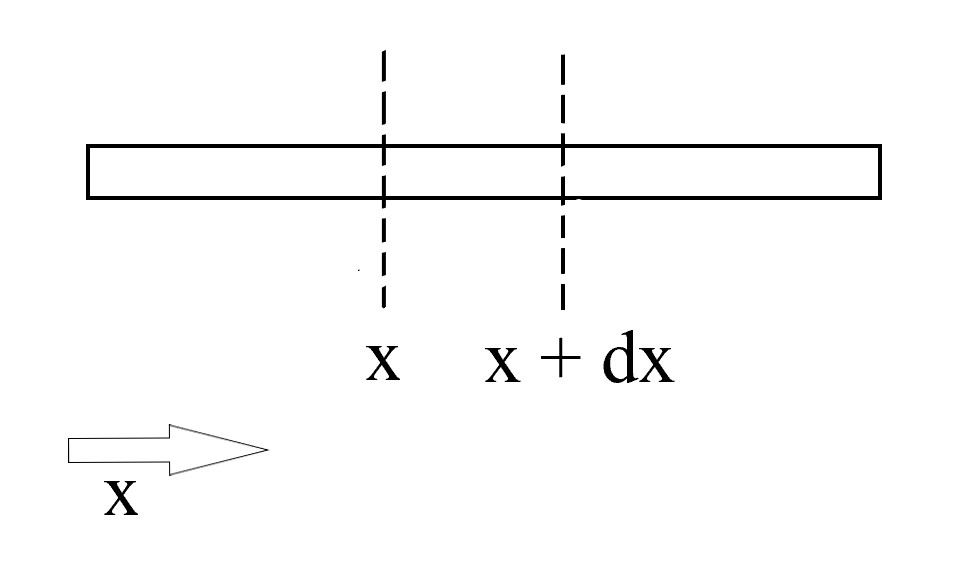
\includegraphics[width=0.275\textwidth]{im01.jpg}
	\caption*{شکل ۱: مدلسازی انتقال حرارت یک بعدی\\
		\large{
		}
	}
\end{figure}

\[(\left.KA\frac{\partial u}{\partial x}\right|_{x+\Delta x}-\left.KA\frac{\partial u}{\partial x}\right|_{x}) \cdot \Delta t=
mc_p \cdot \Big(u(x,t+\Delta t)-u(x,t)\Big)\]
و
\[m=\rho \cdot \Delta v=\rho \cdot  A \cdot \Delta x\]
که در آن $u(x,t)$ دمای نقطه به طول $x$ در لحظه $t$ است. پس
\begin{alignat*}{1}
	&\begin{cases}
		\left.\frac{\partial u}{\partial x}\right|_{x+\Delta x}-\left.\frac{\partial u}{\partial x}\right|_{x} = \frac{\partial^2 u}{\partial x^2}  \cdot \Delta x\\
		u(x,t+\Delta t)-u(x,t)=\frac{\partial u}{\partial t} \cdot \Delta t
	\end{cases} 
	\\& \Rightarrow 
	K A \cdot \frac{\partial^2 u}{\partial x^2}  \Delta x \Delta t=c_p\rho A\frac{\partial u}{\partial t}\Delta t\Delta x
	\\& \Rightarrow
	\frac{\partial u}{\partial t}=\frac{k}{c_p\rho} \cdot \frac{\partial^2 u}{\partial x^2}
\end{alignat*}

پس اگر تعریف کنیم
$\alpha := \frac{k}{c_p\rho}$
متوجه می شویم که\\
\[u_t=\alpha u_{xx}\]
\[u(0,t)=u(L,t)=0\]
\[u(x,0)=f(x)\]
اگر هم این مسئله را در ۲ بعد بررسی کنیم، به دلیل وجود هدایت گرما در هر دو راستای $x$ و $y$ خواهیم داشت\\:
\begin{figure}[H]
	\centering
	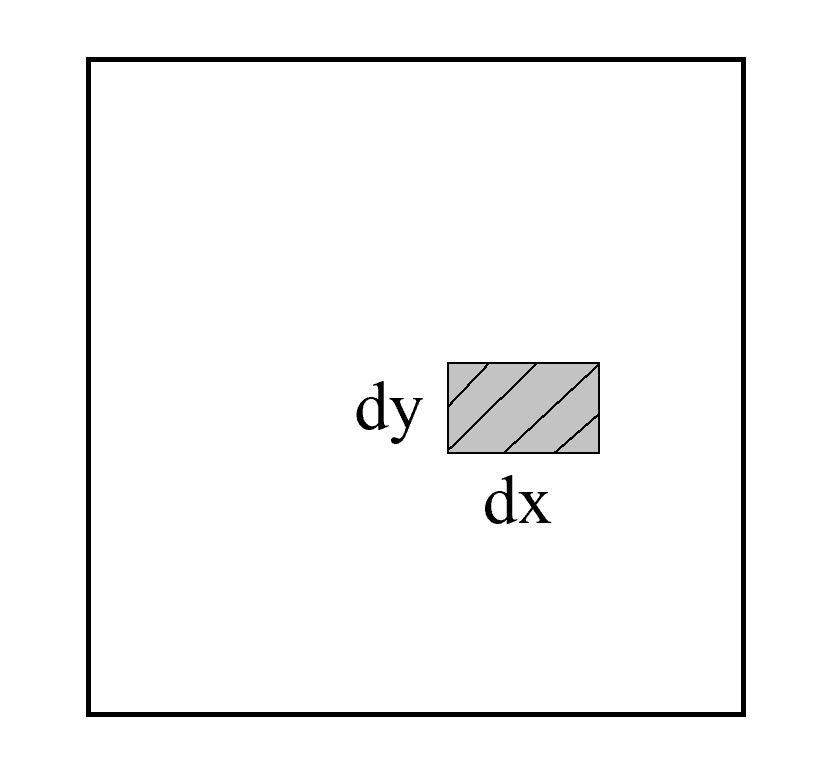
\includegraphics[width=0.275\textwidth]{im02.jpg}
	\caption*{شکل ۲: مدلسازی انتقال حرارت دو بعدی\\
		\large{
		}
	}
\end{figure}


\[\frac{\partial u}{\partial t}=\alpha(\frac{\partial^2 u}{\partial x^2}+\frac{\partial^2 u}{\partial y^2})\]
\subsubsection{
	معادله لاپلاس، انتقال حرارت پایا
	\lr{(steady state)}
}
\begin{equation*}
	\begin{aligned}
		{} &\ \frac{\partial u}{\partial t}=0 \\
		&\ \frac{\partial u}{\partial t}=\alpha(\frac{\partial^2 u}{\partial x^2}+\frac{\partial^2 u}{\partial y^2}) \\
		&\ \Rightarrow \frac{\partial^2 u}{\partial x^2}+\frac{\partial^2 u}{\partial y^2}=0
	\end{aligned}
\end{equation*}
پس داریم
\begin{equation*}
	\begin{aligned}
		{} &\ 
		u_{xx}+u_{yy}=0
		\\
		&\
		u_x(0,y)=u_x(a,y)=0
		\\
		&\
		u(x,0)=f(x)
		\\
		&\
		u(x,b)=g(x)
		\\
	\end{aligned}
\end{equation*}



\subsubsection{موج (نوسان طناب)}
حال مدلسازی نوسان طناب یک بعدی را بررسی می کنیم. چنانچه، طناب دارای طول $L$، جرم $M$ و سختی $K$ باشد و $u(x,t)$ ارتفاع نقطه به طول $x$ در لحظه باشد، بر اساس قانون هوک داریم:
\begin{figure}[H]
	\centering
	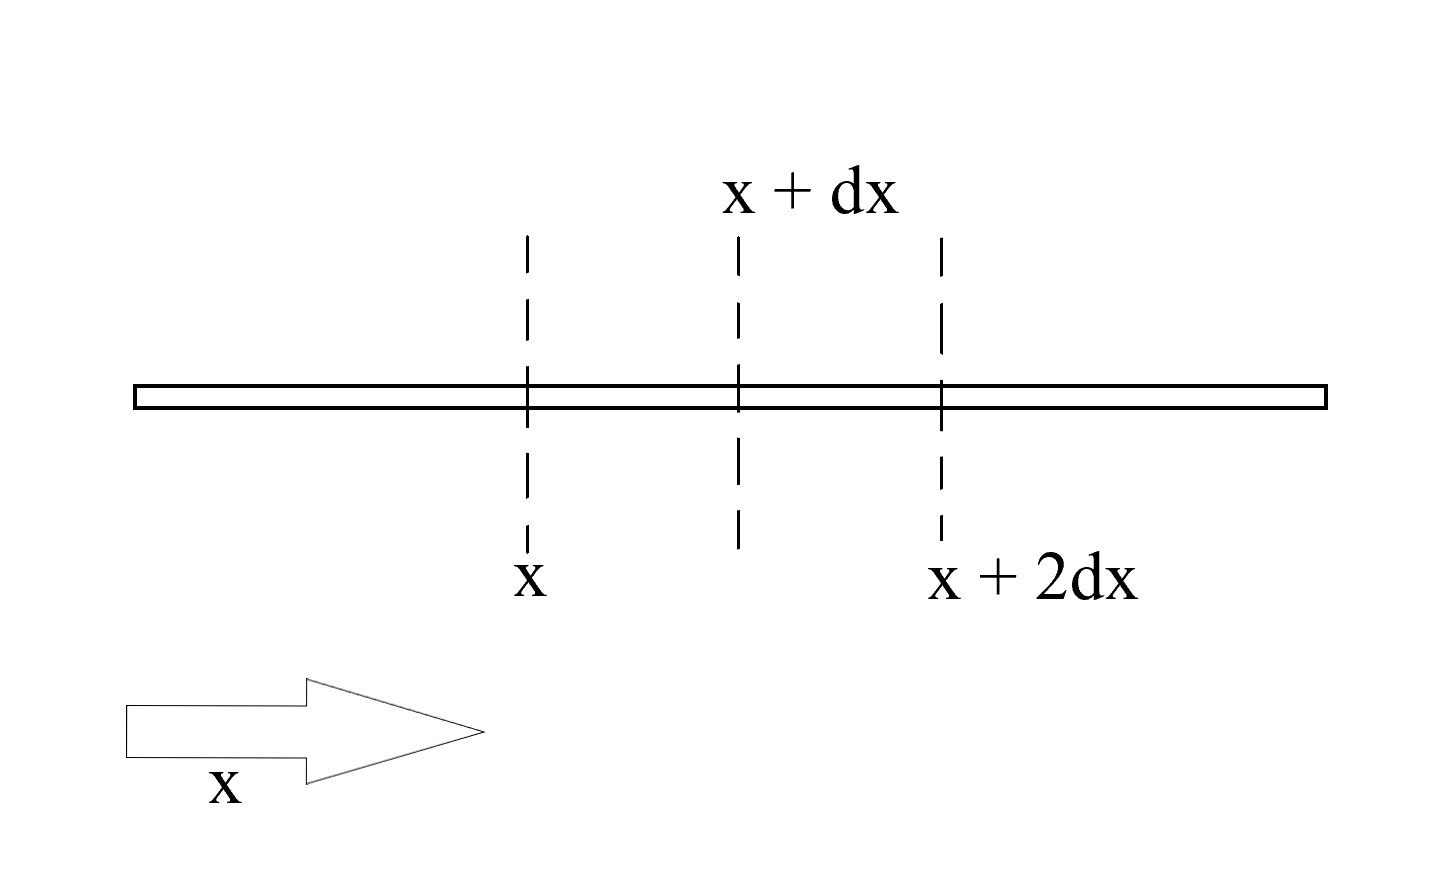
\includegraphics[width=0.275\textwidth]{im03.jpg}
	\caption*{شکل ۳: مدلسازی نوسان یک بعدی\\
		\large{
		}
	}
\end{figure}
\[
F=k[u(x+2\Delta x)-u(x+\Delta x)]-k[u(x+\Delta x)-u(x)]=ma=m\frac{\partial^2 u}{\partial t^2}
\]
همچنین، فرض می کنیم هر المان طناب با طول $dx$ دارای جرم $m$ و سختی $k$ باشد و کل طناب از $n$ المان تشکیل شود.
\begin{figure}[H]
	\centering
	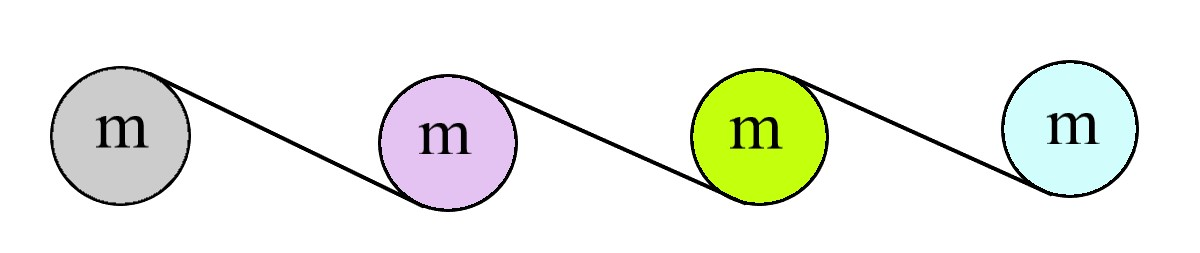
\includegraphics[width=0.275\textwidth]{im04.jpg}
	\caption*{شکل ۴: المان های مورد نیاز برای مدلسازی\\
		\large{
		}
	}
\end{figure}
بنابراین، 
$L=n\Delta x$
و
$M=nm$
و
$K=\frac{k}{n}$
حال با توجه به رابطه قبلی داریم
\begin{equation*}
	\begin{aligned}
		k\Big(u(x+{}&\ 2\Delta x,t)- 2u(x+\Delta x,t)+u(x,t)\Big)=m\frac{\partial^2 u}{\partial t^2}\\
		&\  \Rightarrow  u_{tt}=\frac{k}{m}u_{xx}(\Delta x)^2\\
		&\  \Rightarrow u_{tt}=\frac{k(\Delta x)^2}{m}u_{xx}\\ 
		&\ \Rightarrow u_{tt}=\frac{nK\frac{L^2}{K^2}}{\frac{M}{n}}u_{xx}\\
		&\  \Rightarrow u_{tt}=\frac{KL^2}{M}u_{xx} \\
	\end{aligned}
\end{equation*}
تعریف می کنیم
$c^2 = \frac{KL^2}{M}$
.
پس داریم

\begin{equation*}
	\begin{aligned}
		{}&\ u_{tt}=c^2u_{xx} \\
		&\ u(0,t)=u(L,t)=0 \\
		&\ u(x,0)=f(x) \\
		&\ u_t(x,0)=g(x) \\
	\end{aligned}
\end{equation*}

اگر هم این مسئله را در ۲ بعد بررسی کنیم، خواهیم داشت\\
\begin{figure}[H]
	\centering
	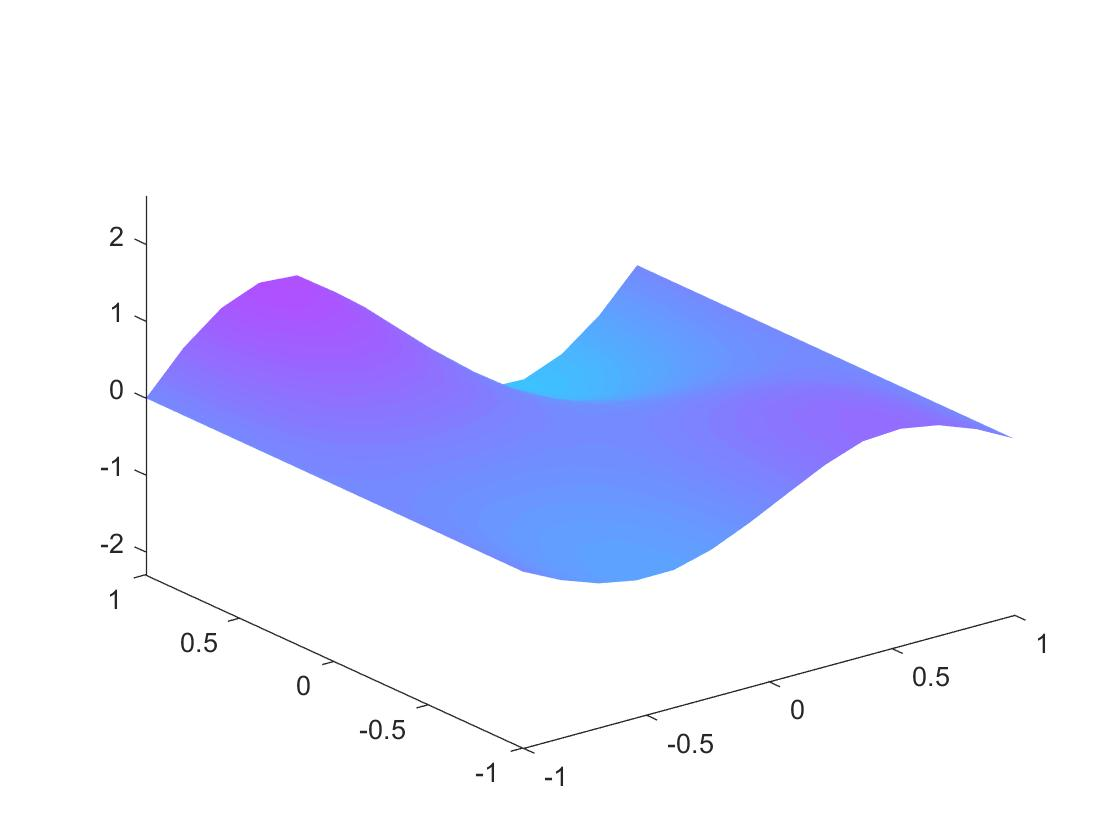
\includegraphics[width=0.275\textwidth]{im05.jpg}
	\caption*{شکل ۵: مدلسازی نوسان دو بعدی\\
		\large{
		}
	}
\end{figure}
\[
u_{tt}=c^2(u_{xx}+u_{yy})
\]

\subsection*{سری فوریه}
۱) تابع پیوسته و متناوب
$f$
با دوره تناوب
$2\pi$\\
اگر 
$f:\R\to\R$
پیوسته و متناوب با دوره ی تناوب 
$2\pi$
باشد، ضرایب
$a_k,a_0$
و
$b_k$
موجودند به طوری که به ازای هر
$x\in\R$
داریم
\begin{equation}
	f(x)=\int_{-\pi}^{\pi}{\frac{a_0}{2}dx}+\sum_{k=1}^\infty {\int_{-\pi}^{\pi}{a_kcos(kx)dx}}+\sum_{k=1}^\infty{\int_{-\pi}^{\pi}{b_ksin(kx)dx}}
\end{equation}
همچنین داریم
\begin{equation}
	a_0=\frac{1}{\pi}\int_{-\pi}^{\pi} {f(x)dx}
\end{equation}
\begin{equation}
	a_k=\frac{1}{\pi}\int_{-\pi}^{\pi} {f(x)cos(kx)dx}
\end{equation}
\begin{equation}
	b_k=\frac{1}{\pi}\int_{-\pi}^\pi {f(x)sin(kx)dx}
\end{equation}


\begin{proof}
	برای محاسبه ضریب
	$a_0$
	، کافی است از طرفین 
	$(5)$
	در بازه ی
	$[-\pi,\pi]$
	انتگرال بگیریم : 
	\[
	\int_{-\pi}^\pi {f(x)dx}=\int_{-\pi}^\pi{\frac{a_0}{2}}dx+\sum_{k=1}^\infty a_k{int_{-\pi}^\pi{cos(kx)dx}}+\sum_{k=1}^\infty b_k{int_{-\pi}^\pi{sin(kx)dx}}
	\]
	همچنین داریم :
	\[
	\int_{-\pi}^\pi{cos(kx)dx}=\left.\frac{sin(kx)}{k}\right |_{-\pi}^\pi=0
	\]
	\[
	\int_{-\pi}^\pi{sin(kx)dx}=0
	\]
	دقت کنید که دلیل رابطه آخر این است که
	$sin(kx)$
	تابعی فرد است و بازه انتگرال گیری متقارن است. بنابراین داریم
	\[
	f(x)=\frac{a_0}{2}(2\pi)+0+0\Rightarrow  a_0=\frac{1}{\pi}\int_{-\pi}^\pi {f(x)dx}
	\]
	حال برای محاسبه ضرایب 
	$a_j$
	، ابتدا طرفین تساوی 
	$(5)$
	را در 
	$cos(jx)$
	ضرب می کنیم و سپس در بازه ی 
	$[-\pi,\pi]$
	انتگرال می گیریم :
	\begin{equation*}
		\begin{aligned}
			\int_{-\pi}^\pi{f(x)cos(jx)dx} {} &\ =\frac{a_0}{2}\int_{-pi}^\pi{cos(jx)dx}+\sum_{k=1}^\infty{\int_{-\pi}^\pi{cos(kx)cox(jx)dx}} \\
			&\ +\sum_{k=1}^\infty{a_k\int_{-\pi}^\pi{cos(kx)cox(jx)dx}} \\
			&\ +\sum_{k=1}^\infty{b_k\int_{-\pi}^\pi{cos(kx)sin(jx)dx}} \\
		\end{aligned}
	\end{equation*}
	از طرفی برای هر عدد صحیح
	$j\ne0$
	داریم
	\[
	\int_{-\pi}^\pi{cos(jx)dx}=\left.{\frac{sin(kx)}{k}}\right |_{-\pi}^\pi=0
	\]
	وبرای هر 
	$j,k$
	صحیح، با توجه به فرد بودن تابع
	$sin(kx)cos(jx)$
	داریم
	\[
	\int_{-\pi}^\pi{sin(kx)cos(jx)dx}=0
	\]
	و همچنین داریم
	\begin{align*}
		\int_{-\pi}^\pi{cos(kx)cox(jx)dx}&=
		\begin{cases}
			\int_{-\pi}^\pi{\frac{1}{2}\Big[cos\big((k+j)x\big)+cos\big((k-j)x\big)\Big]} &\mbox{if } k\ne j\\
			\int_{-\pi}^\pi{\frac{1+cos(2jx)}{2}dx}   
			&\mbox{if } k=j\\
		\end{cases}
		\\
		&=\begin{cases}
			0 &\mbox{if } k\ne j
			\\
			\pi &\mbox{if } k=j
		\end{cases}
	\end{align*}
	و بنابراین متوجه می شویم که برای هر 
	$j\in\N$
	داریم
	\[
	\int_{-\pi}^\pi{f(x)cos(jx)dx} {} = 0+a_j\times\pi+0\Rightarrow a_j=\frac{1}{\pi}\int_{-\pi}^\pi{f(x)cos(jx)dx}
	\]
	به طور مشابه با ضرب طرفین
	$(5)$
	در
	$sin(jx)$
	و انتگرال گیری در بازه
	$[-\pi,\pi]$
	می توان نشان داد که برای هر 
	$j\in\N$
	،
	$b_j=\frac{1}{\pi}\int_{-\pi}^\pi{f(x)sin(jx)dx}$
	است.\\
\end{proof}

\begin{example}
	
	سیگنال مثلثی
	\begin{align*}
		&f(x)=
		\begin{cases}
			\pi-x &\mbox{if  } { 0\le x\le \pi}
			\\
			\pi+x &\mbox{if  }  {-\pi\le x \le 0}
		\end{cases}
		&f(x+2\pi)=f(x)
	\end{align*}
	
	\hrulefill
	
	حل- 
	\begin{equation*}
		\begin{aligned}
			a_0 {} &\ = \frac{1}{\pi}\int_{-\pi}^\pi{f(x)dx}\\
			&\ =\frac{1}{\pi}\left(\int_{-\pi}^0{\pi-x \, dx}+\int_0^\pi{\pi+x \, dx}\right)\\
			&\ =\frac{1}{\pi}\left(
			\left.{\frac{(\pi+x)^2}{2}}\right |_{-\pi}^0
			+
			\left.{\frac{-(\pi-x)^2}{2}}\right |_0^\pi
			\right)\\
			&\ = \frac{1}{\pi}\left(
			\frac{\pi^2}{2}-0+0+\frac{\pi^2}{2}
			\right)= \pi
			\\\\
			a_k {} &\ = \frac{1}{\pi}\int_{-\pi}^\pi{f(x)cos(kx)dx}\\
			&\ = \frac{1}{\pi}\left(
			\int_{-\pi}^{0}{(\pi+x)cos(kx) dx} +\int_{0}^{\pi}{(\pi-x)cos(kx)dx}
			\right)\\
			&\ = \frac{1}{\pi}\left(
			\int_{-\pi}^{0}{xcos(kx) dx} -\int_{0}^{\pi}{(xcos(kx)dx}
			\right)
			+
			\int_{-\pi}^{\pi}{cos(kx)dx}
		\end{aligned}
	\end{equation*}
	
	که در آن 
	\begin{alignat*}{3}
		\int_{-\pi}^{0}{xcos(kx)dx}
		= & \left.{\frac{xsin(kx)}{k}}\right |_{-\pi}^{0} & -\int_{-\pi}^{0}{\frac{sin(kx)}{k}dx}
		&= \frac{1-(-1)^k}{k^2}
		\\
		\int_{0}^{\pi}{xcos(kx)dx}
		= & \left.{\frac{xsin(kx)}{k}}\right |_{0}^{\pi} & -\int_{0}^{\pi}{\frac{sin(kx)}{k}dx}
		&=\frac{(-1)^k-1}{k^2}
		\\
		\int_{-\pi}^{\pi}{cos(kx)dx}=& 0
	\end{alignat*}
	
	بنابراین
	\[
	a_k=\frac{1}{\pi}\frac{2}{k^2}\left(1-(-1)^k\right)=
	\begin{cases}
		0 &\mbox{if } k=2n\\
		\frac{4}{\pi(2n-1)^2} &\mbox{if } k=2n-1
	\end{cases}
	\]
	و
	\begin{equation*}
		\begin{aligned}
			b_k {} &\ = \frac{1}{\pi}\int_{-\pi}^{\pi}{f(x)sin(kx)dx}\\
			&\ = \frac{1}{\pi}\left(
			\int_{-\pi}^{0}{(\pi+x)sin(kx)dx}+\int_{0}^{\pi}{(\pi-x)sin(kx)dx}
			\right)\\
			&\ = \frac{1}{\pi}\left(\int_{-\pi}^{0}{xsin(kx)dx}-\int_{0}^{\pi}{xsin(kx)dx} \right)+\int_{-\pi}^{\pi}{sin(kx)dx}
		\end{aligned}
	\end{equation*}
	که
	\begin{alignat*}{2}
		{} &\ \int_{-\pi}^{0}{xsin(kx)dx}
		=&\left.{-\frac{xcos(kx)}{k}}\right |_{-\pi}^{0} 
		&+\int_{-\pi}^{0}{\frac{cos(kx)}{k}dx}=\frac{\pi(-1)^{k+1}}{k}\\
		&\ \int_{0}^{\pi}{xsin(kx)dx}
		=&\left.{-\frac{xcos(kx)}{k}}\right |_{0}^{\pi} 
		&+\int_{0}^{\pi}{\frac{cos(kx)}{k}dx}=\frac{\pi(-1)^{k+1}}{k}\\
		&\ \int_{-\pi}^{\pi}{sin(kx)dx}=0
	\end{alignat*}
	
	پس 
	$b_k=0$
	است. پس\\
	\[f(x)=\frac{\pi}{2}+\sum_{n=1}^{\infty}{\frac{4}{n(2n-1)^2}}cos(2n-1)x\]
	
\end{example}
\hrulefill

*توجه : نمودار 
$f(x)$
در مثال ۱ بصورت 
\begin{figure}[H]
	\centering
	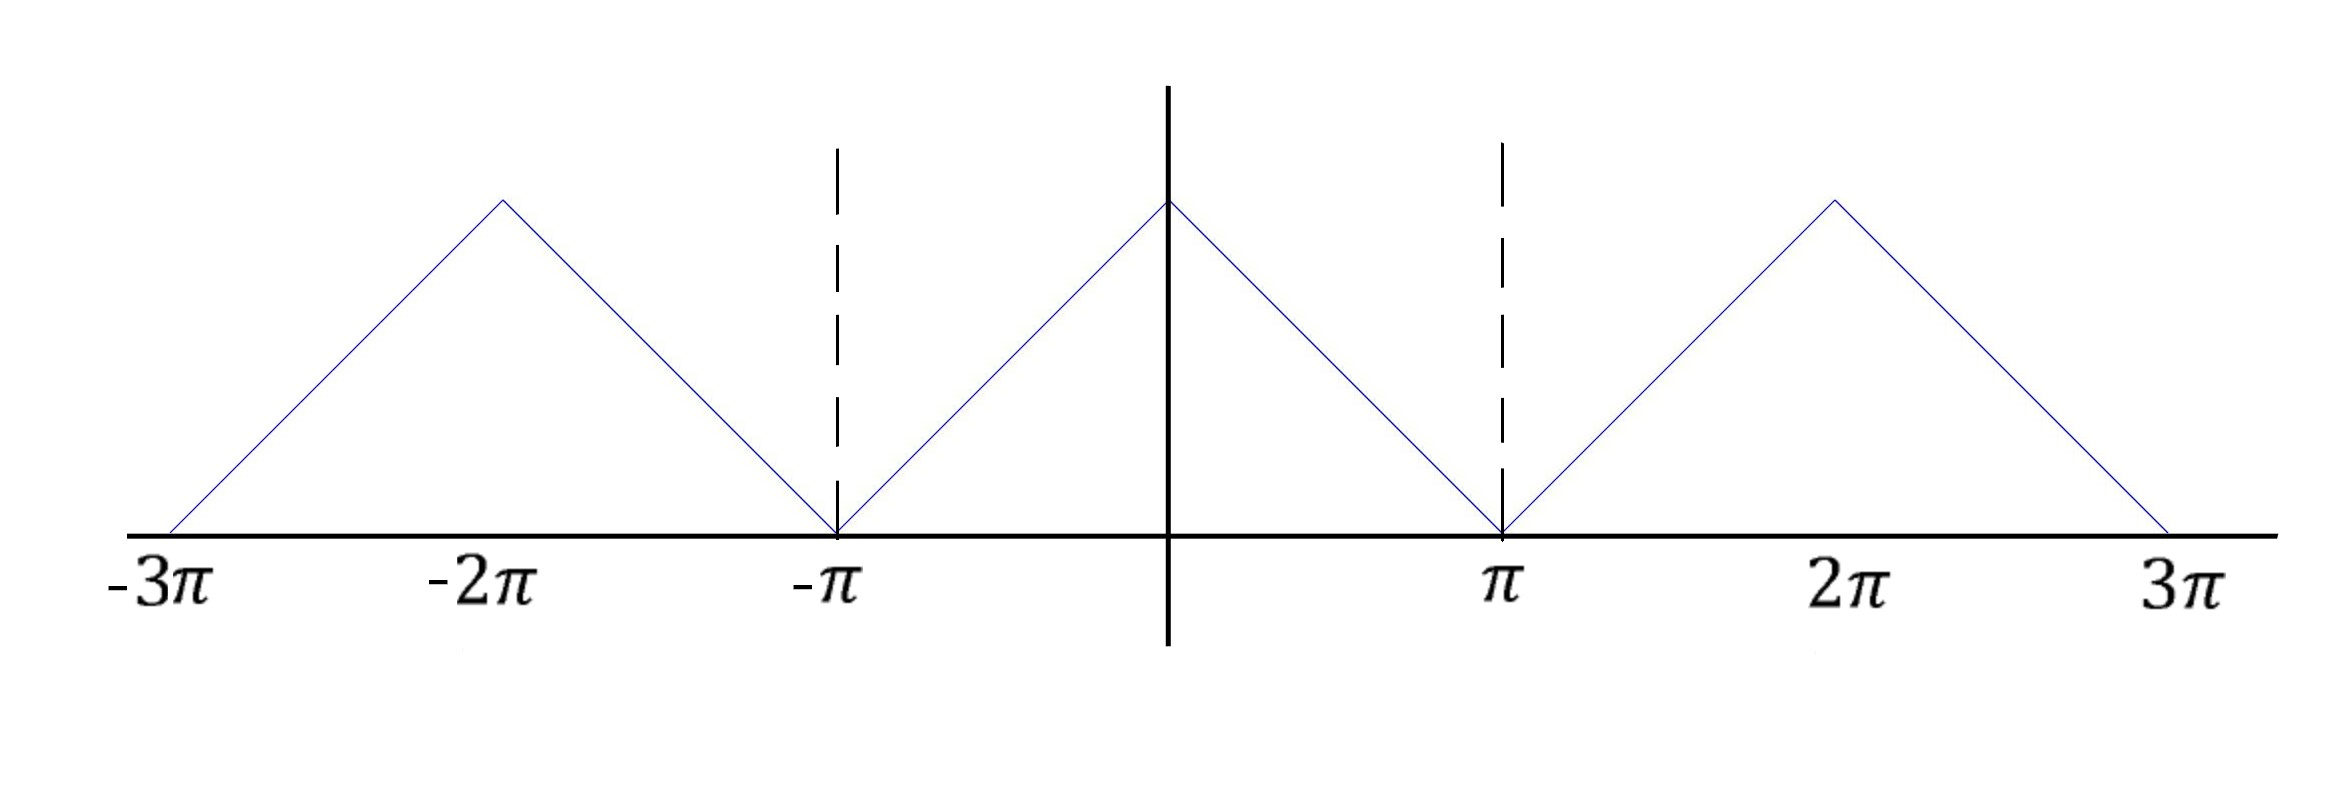
\includegraphics[width=0.275\textwidth]{im06.jpg}
	\caption*{شکل ۶: نمودار موج مثلثی\\
		\large{
		}
	}
\end{figure}
است. بنابراین 
$f(x)$
تابعی زوج است و در رابطه 
$(8)$
از زوج بودن 
$f$
و فرد بودن تابع
$sin(kx)$
نتیجه می شود که 
$b_k=0$.
پس توجه به زوج یا فرد بودن سیگنال 
$f(x)$
محاسبات ضرایب سری فوریه را ساده می کند. بعدا در مورد این نکته مفصل صحبت می کنیم.\\
توجه- اگر تابع 
$f(x)$
پیوسته و با دوره تناوب 
$2\pi$
بوده و در نقطه ی 
$x_0$
دارای ناپیوستگی نوع اول باشد، آنگاه سری فوریه ی
$f$
در
$x_0$
به میانگین حد چپ و راست همگراست.\\

\hrulefill

\begin{example}
	سری فوریه ی تابع
	$f(x)$
	با ضابطه ی زیر را بدست آورید.
	\begin{align*}
		&f(x)=
		\begin{cases}
			0 &\mbox{if } 0\le x\le \pi
			\\
			\pi &\mbox{if } -\pi\le x \le 0
		\end{cases}
		& f(x+2\pi)=f(x)
	\end{align*}
	\hrulefill
	\\
	حل-
	\begin{equation*}
		\begin{aligned}
			{} &\ a_0=\frac{1}{\pi}\int_{-\pi}^{\pi}{f(x)dx}=\frac{1}{\pi}\int_{0}^{\pi}{\pi dx}=\pi\\
			&\ a_k=\frac{1}{\pi}\int_{-\pi}^{\pi}{f(x)cos(kx)dx}=\frac{1}{\pi}\int_{0}^{\pi}{\pi cos(kx) dx}=0\\
			&\ b_k=\frac{1}{\pi}\int_{-\pi}^{\pi}{f(x)sin(kx)dx}=\frac{1}{\pi}\int_{0}^{\pi}{\pi sin(kx) dx}=\frac{1-(-1)^k}{k}\\
		\end{aligned}
	\end{equation*}
	
\end{example}
\hrulefill
حال در 
$x=0$
که نقطه ناپیوستگی است، داریم
$f^+(0)=\pi , f^-(0)=0$
و  سری فوریه در این نقطه به
$\frac{\pi}{2}=\frac{f^+(0)+f^-(0)}{2}$
همگراست.\\
\begin{example}
	تابع زیر را در نظر بگیرید.
	\begin{align*}
		&f(x)=
		\begin{cases}
			-\pi &\mbox{if } -\pi\le x\le 0
			\\
			x &\mbox{if } 0\le x \le \pi
		\end{cases}
		& f(x+2\pi)=f(x)
	\end{align*}
	\hrulefill
	\\
	الف) سری فوریه ی تابع 
	$f(x)$
	را به دست آورید.\\
	ب) نشان دهید 
	$\sum_{k=1}^{\infty}{\frac{1}{(2k+1)^2}}=\frac{\pi^2}{8}$
\end{example}
حل-
\begin{equation*}
	\begin{aligned}
		a_0 {}
		&\
		=\frac{1}{\pi}\int_{-\pi}^{\pi}{f(x)dx}\\
		&\
		=\frac{1}{\pi}\left(\int_{-\pi}^{0}{\pi \, dx}+\int_{0}^{\pi}{x \, dx}\right)=\frac{1}{\pi}\left(\pi^2+\frac{\pi^2}{2}\right)=\frac{3\pi^2}{2}
	\end{aligned}
\end{equation*}
\begin{equation*}
	\begin{aligned}
		a_k {} &\
		=\frac{1}{\pi}\int_{-\pi}^{\pi}{f(x)dx} \\
		&\
		=\frac{1}{\pi}\left(\int_{-\pi}^{0}{\pi cos(kx)dx}+\int_{0}^{\pi}{x cos(kx)dx}\right)
		&\
		=\frac{1}{\pi}\left(-\int_0^\pi{\frac{sin(kx)}{x}dx}\right)=\frac{(-1)^k-1}{k^2\pi}
	\end{aligned}
\end{equation*}
\begin{equation*}
	\begin{aligned}
		b_k {} &\
		=\frac{1}{\pi}\int_{-\pi}^{\pi}{f(x)cos(kx)dx}\\
		&\
		=\frac{1}{\pi}\left(\int_{-\pi}^{0}{\pi sin(kx)dx}+\int_{0}^\pi{xsin(kx)dx}\right)\\
		&\
		=\frac{1}{\pi}\left(\frac{\pi\left((-1)^k-1\right)}{k}-\left.{\frac{xcos(kx)}{k}}\right |_0^\pi+\int_0^\pi{\frac{cos(kx)}{k}dx}\right)\\
		&\
		=\frac{1}{\pi}\left(\frac{\pi\left((-1)^k-1\right)}{k}-\frac{\pi(-1)^k}{k}+0\right)=-\frac{1}{k}
	\end{aligned}
\end{equation*}
پس در نقاط پیوستگی 
$f$
داریم
\[
f(x)=\frac{3\pi}{4}+\sum_{k=1}^\infty{\frac{(-1)^k-1}{k^2\pi}cos(kx)}+\sum_{k=1}^\infty{-\frac{1}{k}sin(kx)}
\]
و در نقاط ناپیوستگی 
$f$
شامل
$x_0=2k\pi$
داریم 
$cos(kx_0)=1,sin(kx_0)=0$
پس در این نقطه داریم
\begin{equation}
	\text{سری فوریه}=
	\frac{3\pi}{4}+\sum_{k=1}^\infty{\frac{(-1)^k-1}{k^2\pi}}
\end{equation}
همچنین 
$f^-(x_0)=\pi$
و
$f^+(x_0)=0$
و بنابراین 
\begin{equation}
	\text{سری فوریه}=
	\frac{0+\pi}{2}=\pi/2
\end{equation}
و از ترکیب تساوی
$(9)$
و
$(10)$
نتیجه می شود که
\[
\frac{3\pi}{4}+\sum_{k=1}^\infty{\frac{(-1)^k-1}{k^2\pi}}=\frac{\pi}{2}\Rightarrow
\sum_{k=1}^\infty{\frac{2}{(2k-1)^2\pi}}=\frac{\pi}{4}\Rightarrow
\sum_{k=1}^\infty{\frac{1}{(2k-1)^2}}=\frac{\pi^2}{8}
\]
۲) تابع متناوب
$f$
با دوره تناوب
$2L$\\
اگر
$f:\R\to\R$
متناوب با دوره ی تناوب 
$2L$
باشد، ضرایب 
$a_k,a_0$
و
$b_k$
موجودند به طوری که\\
الف) در نقاط پیوستگی 
$x$
\[
f(x)=\frac{a_0}{2}+\sum_{k=1}^\infty{a_kcos\left(\frac{k\pi}{L}\right)dx}+\sum_{k=1}^\infty{b_ksin\left(\frac{k\pi}{L}\right)dx}
\]
ب) و در نقاط ناپیوستگی نوع اول
$\tilde{x}$
\[
\frac{f^-(x_0)+f^+(x_0)}{2}=\frac{a_0}{2}+\sum_{k=1}^\infty{a_kcos\left(\frac{k\pi}{L}x\right)dx}+\sum_{k=1}^\infty{b_ksin\left(\frac{k\pi}{L}x\right)dx}
\]
همچنین داریم
\[
a_0=\frac{1}{L}\int_{-L}^L{f(x)dx}
\]
\[
a_k=\frac{1}{L}\int_{-L}^L{f(x)cos\left(\frac{k\pi}{L}x\right)dx}
\]
\[
b_k=\frac{1}{L}\int_{-L}^L{f(x)sin\left(\frac{k\pi}{L}x\right)dx},
\]
اثبات- برای اثبات کافی است با یک تغییر متغیر خطی مناسب دوره تناوب را به
$2\pi$
تبدیل کنیم. قرار می دهیم
$t=\frac{\pi}{L}x$.
در این صورت داریم
\[
f(x)=f(\frac{L}{\pi}t)=g(t)
\]
و 
$g$
دارای دوره تناوب 
$2\pi$
است، زیرا :
\[
g(t+2\pi)=f\left(\frac{L}{\pi}\left(t+2\pi\right)\right)=f\left(\frac{L}{\pi}t+2L\right)=f\left(\frac{L}{\pi}t\right)=g(t)
\]
بنابراین
$g(t)$
دارای سری فوریه ای به فرم
\begin{equation}
	g(t)=\frac{a_0}{2}+\sum_{k=1}^\infty{a_kcos(kt)}+\sum_{k=1}^\infty{b_ksin(kt)}
\end{equation}
است که در آن
\[
a_0=\frac{1}{\pi}\int_{-\pi}^\pi{g(t)dt}
\]
\[
a_k=\frac{1}{\pi}\int_{-\pi}^\pi{g(t)cos(kt)dt)}
\]
\[
b_k=\frac{1}{\pi}\int_{-\pi}^\pi{g(t)sin(kt)dt}
\]
است.\\
حال کافی است در
$(11)$
متغیر
$t$
را دوباره به 
$x$
تبدیل کنیم. بنابراین
\[
f(x)=g(t)=\frac{a_0}{2}+\sum_{k=1}^\infty{a_kcos\left(\frac{k\pi}{L}\right)dx}+\sum_{k=1}^\infty{b_ksin\left(\frac{k\pi}{L}\right)dx}
\]
\[
a_0=\frac{1}{\pi}\int_{-\pi}^\pi{g(t)dt}=
\frac{1}{\pi}\int_{-L}^L{g\left(\frac{\pi}{L}x\right)\frac{\pi}{L}x \, dx}=\frac{1}{\pi}\int_{-L}^L{\frac{\pi}{L}f(x)dx}=
\frac{1}{L}\int_{-L}^L{f(x)dx}
\]
و به طور مشابه روابط
$a_k$
و
$b_k$
نیز اثبات می شود.\\
مثال- سری فوریه ی همگرا به تابع زیر را بدست آوردید و در نقاط ناپیوستگی مقدار همگرایی را به دست آورید.
\begin{equation*}
	\begin{gathered}
		x \quad \text{if } -1\le x\le 1
		\\
		f(x+2)=f(x)
	\end{gathered}
\end{equation*}
حل-
\begin{equation*}
	\begin{aligned}
		{} &\
		2L=2\Rightarrow L=1
		\\ &\
		a_0=\frac{1}{1}\int_{-1}^1{f(x)dx}=\int_{-1}^1{x \, dx}=0
		\\ &\
		a_k=\frac{1}{1}\int_{-1}^1{f(x)cos(k\pi x)dx}=\int_{-1}^1{xcos(k\pi x)dx}=0 
		\\ &\ \begin{aligned}
			b_k {} &\
			=\frac{1}{1}\int_{-1}^1{f(x)sin(k\pi x)dx}=\int_{-1}^1{sin(k\pi x)dx}=\left. {-\frac{xcos(k\pi x)}{k\pi}}\right |_{-1}^1+\int_{-1}^1{\frac{cos(k\pi x)}{k}dx}
			\\ &\ 
			= \frac{(-1)^{k+1)}}{k\pi}+\frac{(-1)^{k+1)}}{k\pi}+0=\frac{2(-1)^{k+1)}}{k\pi}
		\end{aligned}
	\end{aligned}
\end{equation*}
پس در نقاط پیوستگی داریم
\[
f(x)=\sum_{k=1}^{\infty}{\frac{2(-1)^{k+1}}{k\pi}sin(k\pi x)}
\]
و در نقاط ناپیوستگی
$\tilde{x}=n$
داریم 
\[
\forall k\in\N: sin(k\pi \tilde{x})=0\Rightarrow f(\tilde{x})=0
\]
همچنین داریم
$f^-\left(\tilde{x}\right)=-1 ,f^-\left(\tilde{x}\right)=1$
پس
\[
f\left(\tilde{x}\right)=\frac{f^-\left(\tilde{x}\right)+f^+\left(\tilde{x}\right)}{2}
\]
* توجه - همان طور که در مثال قبل دیدیم، فرد بودن تابع 
$f$
باعث شد که ضرایب
$a_0$
و 
$a_k$
سری فوریه صفر شوند. به طور کلی زوج یا فرد بودن تابع محسابات ضرایب سری فوریه را کوتاه تر می کند. در ادامه این بحث را دقیق تر بررسی می کنیم.\\
* تابع زوج 
$f$
با دوره تناوب
$2L$
\begin{equation*}
	\begin{aligned}
		{} &\
		a_0=\frac{1}{L}\int_{-L}^L{f(x)dx}=\frac{2}{L}\int_{0}^L{f(x)dx}
		\\ &\
		a_k=\frac{1}{L}\int_{-L}^L{f(x)cos\left(\frac{k\pi}{L}x\right)dx}=\frac{2}{L}\int_{0}^L{f(x)cos\left(\frac{k\pi}{L}x\right)dx}
		\\ &\
		b_k=\frac{1}{L}\int_{-L}^L{f(x)sin\left(\frac{k\pi}{L}x\right)dx}=0
	\end{aligned}
\end{equation*}
بنابراین روابط فوق برای توابع زوج محاسبه ی ضریب سری فوریه را ساده می کنند.\\
* تابع فرد 
$f$
با دوره تناوب 
$2L$
\begin{equation*}
	\begin{aligned}
		{} &\
		a_0=\frac{1}{L}\int_{-L}^L{f(x)dx}=0
		\\ &\
		a_k=\frac{1}{L}\int_{-L}^L{f(x)cos\left(\frac{k\pi}{L}x\right)dx}=0
		\\ &\
		b_k=\frac{1}{L}\int_{-L}^L{f(x)sin\left(\frac{k\pi}{L}x\right)dx}=\frac{2}{L}\int_{0}^L{f(x)sin\left(\frac{k\pi}{L}x\right)dx}
	\end{aligned}
\end{equation*}
مثال- سری فوریه ی تابع
$f$
با ضابطه ی زیر را بدست آورید.
\begin{equation*}
	\begin{gathered}
		f(x) =
		\begin{cases}
			x       & \quad \text{if }\;\; 0\le x\le 2 \\
			-x  & \quad \text{if }\;\; -2\le x< 0
		\end{cases}\\
		f(x+4)=f(x)
	\end{gathered}
\end{equation*}
حل- تابع زوج است و بنابراین برای محاسبه ی ضرایب سری فوریه داریم :
\begin{equation*}
	\begin{aligned}
		{} &\
		2L=4\Rightarrow L=2
		\\ &\
		a_0=\frac{2}{2}\int_0^2{f(x)dx}=\frac{2}{2}\int_0^2{2 \, dx}=2
		\\ &\
		\begin{aligned}
			a_k {} &\
			= \frac{2}{2}\int_0^2{f(x)cos\left(\frac{k\pi}{2}x\right)dx}=
			\frac{2}{2}\int_0^2{x\,cos\left(\frac{k\pi}{2}x\right)dx}
			\\ &\
			=\left.{\frac{2}{k\pi}x \, sin\left(\frac{k\pi}{2}x\right)}\right |_0^2-\int_0^2{\frac{2}{k\pi} sin\left(\frac{k\pi}{2}x\right)}
			\\ &\
			0+\frac{4}{k^2\pi^2}\left.{cos\left(\frac{k\pi}{2}x\right)} \right |_0^2
			=\frac{4}{k^2\pi^2}\left( (-1)^k-1\right)
		\end{aligned}
		\\ &\
		b_k = 0
		\\ &\
		\implies f(x)=1+\sum_{k=1}^\infty{\frac{4}{k^2\pi^2}\left( (-1)^k-1\right)cos\left( \frac{k\pi}{2}x\right)}
	\end{aligned}
\end{equation*}
*کاربرد سری فوریه در حل معادلات پاره ای\\
در بخش دوم خواهیم دید که در حل معادلات پاره ای با استفاده از روش جداسازی لازم است برای تابع داده شده ی
$f(x)$
سری فوریه ای به دست آوریم که در بازه ی
$[0,L]$
به آن همگرا باشد. در  بعضی از موارد لازم است این سری فوریه فقط شامل جملات سینوسی یا کسینوسی باشد. نحوه ی محاسبه چنین سری فوریه ای را در ادامه می بینیم.\\
۱)سری فوریه ی کسینوسی که در بازه ی
$[0,L]$
به 
$f(x)$
همگراست.\\
با توجه به اینکه می خواهیم سری فوریه فقط شامل جملات کسینوسی باشد، لازم است یک گسترش زوج برای 
$f(x)$
در نظر بگیریم که در بازه ی
$[0,L]$
با 
$f$
برابر باشد.\\
فرض می کنیم 
$g(x)$
یک تابع زوج با دوره تناوب
$2L$
باشد که در بازه ی
$[0,L]$
با 
$f(x)$
برابر است. در این صورت:\\
۱) سری فوریه ی 
$g$
فقط شامل جملات کسینوسی است.\\
۲)این سری فوریه (با فرض پیوستگی
$g$
)
در بازه ی
$[-L,L]$
به
$g$
و در نتیجه در بازه ی
$[0,L]$
به
$f(x)$
همگراست.\\
قرار می دهیم
\begin{equation*}
	\begin{gathered}
		g(x) =
		\begin{cases}
			f(x)       & \quad \text{if }\;\; 0\le x\le L \\
			f(-x)  & \quad \text{if }\;\; -L\le x< 0
		\end{cases}\\
		g(x+2L)=g(x)
	\end{gathered}
\end{equation*}
در این صورت، در نقاط پیوستگی 
$g$
داریم
\begin{equation*}
	\begin{aligned}
		{} &\
		g(x)=\frac{a_0}{2}+\sum_{k=1}^\infty{a_k \, cos\left(\frac{k\pi}{L}x\right)}
		\\ &\
		a_0=\frac{2}{L}\int_0^{L}{g(x)dx}=\frac{2}{L}\int_0^{L}{f(x)dx}
		\\ &\
		a_k=\frac{2}{L}\int_0^L{g(x)cos\left(\frac{k\pi}{L}x\right)dx}=\frac{2}{L}\int_0^L{f(x)cos\left(\frac{k\pi}{L}x\right)dx}
	\end{aligned}
\end{equation*}
و به ازای هر 
$x$
در بازه ی
$[0,L]$
داریم
\[
f(x)=\frac{a_0}{2}+\sum_{k=1}^{\infty}{a_k\, cos\left(\frac{k\pi}{L}x\right)}
\]
که در آن
\begin{equation*}
	\begin{aligned}
		{} &\
		a_0=\frac{2}{L}\int_0^{L}{f(x)dx}
		\\ &\
		a_k=\frac{2}{L}\int_0^L{f(x)cos\left(\frac{k\pi}{L}x\right)dx}
	\end{aligned}
\end{equation*}
۲) سری فوریه ی سینوسی که در بازه ی
$[0,L]$
به
$f(x)$
همگراست.\\
در این حالت لازم است یک گسترش فرد برای
$f(x)$
معرفی کنیم که در بازه ی
$[0,L]$
با 
$f(x)$
برابر باشد.\\
قرار می دهیم
\begin{equation*}
	\begin{gathered}
		h(x) =
		\begin{cases}
			f(x)       & \quad \text{if }\;\; 0\le x\le L \\
			-f(-x)  & \quad \text{if }\;\; -L\le x< 0
		\end{cases}\\
		h(x+2L)=h(x)
	\end{gathered}
\end{equation*}
در این صورت
$h(x)$
دارای سری فوریه ای سینوسی است که در بازه ی
$[0,L]$
به
$f(x)$
همگراست. بنابراین،
\begin{equation*}
	\begin{aligned}
		{} &\
		h(x)=\sum_{k=1}^\infty{b_k \, sin\left(\frac{k\pi}{L}x\right)}
		\\ &\
		b_k=\frac{2}{L}\int_0^L{f(x)sin\left(\frac{k\pi}{L}x\right)dx}
	\end{aligned}
\end{equation*}
و به ازای هر 
$x\in[0,L]$
داریم :
\[
f(x)=\sum_{k=1}^\infty{b_k \, sin\left(\frac{k\pi}{L}x\right)}
\]
که در آن
$b_k=\frac{2}{L}\int_0^L{f(x)sin\left(\frac{k\pi}{L}x\right)dx}$.\\
۳) سری فوریه ای که در بازه ی
$[-L,L]$
به
$f(x)$
همگراست.\\
در این حالت، سر فوریه ی مورد نظر کامل است. بنابراین گسترش متناوب
$f(x)$
کاراتس. متناوب 
$g(x)$
را به این صورت در نظر می گیریم که
\begin{equation*}
	\begin{gathered}
		g(x)=f(x)\quad x\in[L,-L] \\g(x+2L)=g(x)
	\end{gathered}
\end{equation*}
در این صورت 
$g(x)$
دارای سری فوریه ای است که در بازه ی
$[-L,L]$
به 
$f(x)$
همگراست و داریم :
\begin{equation*}
	\begin{aligned}
		{} &\
		f(x)=\frac{a_0}{2}+\sum_{k=1}^\infty{a_k \, cos\left(\frac{k\pi}{L}x\right)}+\sum_{k=1}^\infty{b_k \, sin\left(\frac{k\pi}{L}x\right)}
		\\ &\
		a_0=\frac{1}{L}\int_{-L}^{L}{f(x)dx}
		\\ &\
		a_k=\frac{1}{L}\int_{-L}^L{f(x)cos\left(\frac{k\pi}{L}x\right)dx}
		\\ &\
		b_k=\frac{1}{L}\int_{-L}^L{f(x)sin\left(\frac{k\pi}{L}x\right)dx}
	\end{aligned}
\end{equation*}
*تبدیل فوریه\\
در بخش قبل دیدیم که برای حل معادلات پاره ای در بازه ی
$[0,L]$
از سری فوریه استفاده می کنیم. چنانچه دامنه ی حل معادله ی پاره ای نامتناهی
$(-\infty,\infty)$
یا نیمه نامتناهی
$(0,\infty)$
باشد، برای حل معادلات پاره ای به تبدیل فوریه نیاز داریم.\\
ابتدا تابع پیوسته
$f$
با گسترش زوج در بازه ی
$[-L,L]$
را در نظر می گیریم. در این صورت داریم:
\begin{equation*}
	\begin{aligned}
		{} &\
		f(x)=\frac{a_{0}}{2}+\sum_{k=1}^{\infty} a_{k} \cos \frac{k \pi}{L} x
		\\ &\
		a_{0}=\frac{2}{L} \int_{0}^{L} f(x) d x
		\\ &\
		a_{k}=\frac{2}{L} \int_{0}^{L} f(x) \cos \left(\frac{k \pi}{L} x\right) d x
		\\ &\
		\implies f(x) = \frac{1}{L} \int_{0}^{L} {f(v) dv}+\sum_{k=1}^{\infty} {\frac{2}{L} \int_{0}^{L} {f(v) \cos \left(\frac{k \pi}{L} v\right) \cos \left(\frac{k \pi}{L} x\right) d v}}
	\end{aligned}
\end{equation*}
حال برای مدل کردن دامنه ی نیمه متناهی 
$(0,\infty)$
، حالت حدی 
$L\to \infty$
را در نظر می گیریم. به علاوه فرض می کنیم که
$\int_0^\infty{f(v)dv}$
کراندار باشد. در این صورت داریم :
\[
f(x)=lim_{L\to\infty}{\frac{1}{L}\int_0^L{f(v)dv}}+\sum_{k=1}^{\infty} {\lim _{L\to{\infty}} \frac{2}{L} \int_{0}^{\infty} {f(v) \cos \left(\frac{k \pi}{L} v\right) \cos \left(\frac{k \pi}{L} x\right) d v}}
\]
با انتخاب
$\omega_k=\frac{k\pi}{L}$
داریم
$\Delta\omega=\frac{\pi}{L}$
و بنابراین
\[
f(x)=\sum_{k=1}^{\infty} \lim \frac{2} {\pi} \Delta \omega \int_{0}^{\infty} f(v) \cos \left( \omega_{k} v\right)\cos \left( \omega_{k} x\right)  d v
\]
پس اگر قرار دهیم
\[
g\left(\omega_k\right)=f(v) \cos \left( \omega_{k} v\right)\cos \left( \omega_{k} x\right)  d v
\]
خواهیم داشت
\[
f(x)=\sum_{k=1}^{\infty}\frac{2} {\pi} \lim_{L\to{\infty}} g( \omega_{k} )  \Delta \omega =\frac{2} {\pi} \int_{0}^{{\infty}} g( \omega_{k} )  d \omega=\frac{2} {\pi} \int_{0}^{{\infty}}\int_{0}^{{\infty}} f(v) \cos ( \omega_{k} v)\cos ( \omega_{k} x)  d v\, d\omega
\]
بنابراین در 
$L\to\infty$
با فرض کراندار بودن
$\int_0^\infty{f(v)dv}$
داریم
\begin{equation}
	f(x)=\frac{2} {\pi} \int_{0}^{{\infty}}\int_{0}^{{\infty}} f(v) \cos ( \omega_{k} v)\cos ( \omega_{k} x)  d v d\omega
\end{equation}
تبدیل فوریه ی کسینوسی تابع
$f(x)$
را تعریف می کنیم
\[
F_{C}\{f(x)\}=\sqrt{\frac{2}{\pi}} \int_{0}^{\infty} f(v) \cos (\omega v) d v=F(\omega)
\]
%todo : color
و تبدیل فوریه ی کسینوسی وارون تابع 
$f(x)$
را به صورت
\[
F^{-1}_{C}\{F_{C}\{f(x)\}=\sqrt{\frac{2}{\pi}} \int_{0}^{\infty}\{F_{C}\{f(x)\} \cos (\omega x) d \omega=F(x)
\]
%todo : color
در نظر می گیریم. از
$(12)$
نتیجه می شود که
\[
f(x)=\sqrt{\frac{2}{\pi}} \int_{0}^{\infty}(\sqrt{\frac{2}{\pi}} \int_{0}^{\infty}\ f(v) \cos ( \omega_{k} v)  d v)\cos ( \omega_{k} x) d\omega
\]
و
\[
f(x)=F^{-1}_{C}\{F_{C}\{f(x)\}
\]
به طور مشابه برای تابع 
$f$
در دامنه ی
$(0,\infty)$
تبدیل فوریه ی سینوسی و وارون آن به صورت زیر تعریف می شوند:
\begin{equation*}
	\begin{aligned}
		{} &\
		F_{s}\{f(x)\}=\sqrt{\frac{2}{\pi}} \int_{0}^{\infty} f(v) \sin ( \omega v)  d v
		\\ &\
		F^{-1}_{s}\{F_{s}\{f(x)\}\}=\sqrt{\frac{2}{\pi}} \int_{0}^{\infty} F_{s}\{f(x)\} \sin ( \omega x)  d\omega
	\end{aligned}
\end{equation*}
برای 
$f(x)$
با دامنه ی نامتناهی
$(-\infty,\infty)$
تبدیل فوریه ی نمایی به کار می رود.\\
ابتدا تابع پیوسته و متناوب 
$f$
با دوره تناوب 
$2L$
را در نظر می گیریم و سپس حالت حدی
$L\to\infty$
را بررسی می کنیم.\\
$f$
دارای سری فوریه ای به صورت
\[
f(x)=\frac{a_{0}}{2}+\sum_{k=1}^{\infty} a_{k} \cos \frac{k \pi}{L} x+\sum_{k=1}^{\infty} b_{k} \sin \frac{k \pi }{L}x
\]
است. با جایگذاری ضرایب
$a_k,a_0$
و
$b_k$
نتیجه می شود که
\begin{equation*}
	\begin{aligned}
		f(x)
		{} &\
		=\frac{1}{2 L} \int_{-L}^{L} f(v) d v \\ &\ + \sum_{k=1}^{\infty}\frac{1}{ L} \int_{-L}^{L} f(v) \cos \frac{k \pi}{L} v \cos \frac{k \pi}{L}xdv \\ &\ + \sum_{k=1}^{\infty}\frac{1}{ L} \int_{-L}^{L} f(v) \sin \frac{k \pi}{L} v \sin \frac{k \pi}{L}xdv
	\end{aligned}
\end{equation*}
با قرار دادن
$\omega_k=\frac{k\pi}{L}$
،
$\Delta\omega=\frac{\pi}{L}$
،
$L\to\infty$
و با فرض کران دار بودن
$\int_{-\infty}^\infty{f(v)dv}$
اگر تعریف کنیم
\[
g\left(\omega_k\right)=f(v)(\cos  \omega_{k} v \cos  \omega_{k} x+\sin \omega_{k} v \sin \omega_{k} x) d v
\]
داریم
\begin{equation*}
	\begin{aligned}
		f(x) {} &\ =
		\sum_{k=1}^{\infty} \lim _{l\to \infty} \frac{1}{\pi} \Delta w(\int_{-{\infty}}^{{\infty}} f(v)(\cos  \omega_{k} v \cos  \omega_{k} x+\sin \omega_{k} v \sin \omega_{k} x) d v)
		\\ &\
		=\sum_{k=1}^{\infty} \lim _{l \to\infty} \frac{1}{\pi} \Delta w g(\omega_{k}) 
		\\ &\
		= \frac{1}{\pi}\int_{0}^{{\infty}}g(\omega) d\omega
		\\ &\
		= \frac{1}{\pi}\int_{0}^{{\infty}}\int_{-{\infty}}^{{\infty}} f(v)(\cos  \omega_{k} v \cos  \omega_{k} x+\sin \omega_{k} v \sin \omega_{k} x) d v \ d\omega
		\\ &\
		= \frac{1}{\pi}\int_{0}^{{\infty}}\int_{-{\infty}}^{{\infty}} f(v)\cos(  \omega_{k}(x-v) ) d v \ d\omega
	\end{aligned}
\end{equation*}
دقت می کنیم که تابع داخل انتگرال نسبت به
$\omega$
زوج است و در نتیجه داریم
\[
f(x)= \frac{1}{2\pi}\int_{-{\infty}}^{{\infty}}\int_{-{\infty}}^{{\infty}} f(v)\cos(  \omega(x-v) ) d v \ d\omega
\]
همچنین انتگرال
$\int_{-\infty}^\infty{f(v)sin\left(\omega(x-v)\right)d\omega}\quad$
برابر با صفر است (به دلیل فرد بودن تابع نسبت به
$\omega$
و متقارن بودن بازه
).
پس داریم
\begin{equation}
	f(x)= \frac{1}{2\pi}\int_{-{\infty}}^{{\infty}}\int_{-{\infty}}^{{\infty}} f(v)\cos(  \omega(x-v) ) d v \ d\omega
\end{equation}
\begin{equation}
	0= \frac{1}{2\pi}\int_{-{\infty}}^{{\infty}}\int_{-{\infty}}^{{\infty}} f(v)\sin(  \omega(x-v) ) d v \ d\omega
\end{equation}
با جمع رابطه
$(13)$
با
$(14)\times i$
نتیجه می شود که
\begin{equation*}
	\begin{aligned}
		f(x) {} &\
		= \frac{1}{2\pi}\int_{-{\infty}}^{{\infty}}\int_{-{\infty}}^{{\infty}} f(v)(\cos(\omega(x-v)) +isin(  \omega(x-v)) ) d v \ d\omega
		\\ &\
		=\frac{1}{2\pi}\int_{-{\infty}}^{{\infty}}\int_{-{\infty}}^{{\infty}} f(v) \ e^{i\omega(x-v)} d v \ d\omega
		\\ &\
		=\frac{1}{2\pi}\int_{-{\infty}}^{{\infty}}\int_{-{\infty}}^{{\infty}} f(v) \ e^{i\omega x} e^{-i\omega v} d v \ d\omega
	\end{aligned}
\end{equation*}
و کافی است تبدیل فوریه ی
$f$
و وارون آن را به صورت
\[
F\{f(x)\}=\frac{1} {\sqrt{2\pi}}\int_{-{\infty}}^{{\infty}} f(v) \ e^{-i\omega v} d v
\]
و
\[
F^{-1}\{F\{f(x)\}\}=\frac{1} {\sqrt{2\pi}}\int_{-{\infty}}^{{\infty}}F\{f(x)\} \ e^{i\omega x} d \omega
\]
تعریف کنیم که نتیجه می شود
\[
f(x)=F^{-1}\{F\{f(x)\}\}
\]
مثال- تبدیل فوریه ی کسینوسی و سینوسی تابع 
$f(x)$
با ضابطه زیر را محاسبه کنید.
\[
f(x) =
\begin{cases}
	1       & \quad 0\le x\le 1 \\
	0  & \quad 1<x
\end{cases}
\]
حل-
\begin{equation*}
	\begin{aligned}
		F_{c}\{f(x)\} {} &\
		=\sqrt \frac{2}{\pi}\int_{0}^{{\infty}} f(v)\ cos(\omega v)  d v
		\\ &\
		=\sqrt \frac{2}{\pi}\int_{0}^{1}\ cos(\omega v)  d v=\left.\sqrt \frac{2}{\pi}\frac{ sin(\omega v)}{\omega} \right]_{0}^{1}=\sqrt \frac{2}{\pi}\frac{ sin(\omega )}{\omega}
	\end{aligned}
\end{equation*}
\begin{equation*}
	\begin{aligned}
		F_{s}\{f(x)\} {} &\
		=\sqrt \frac{2}{\pi}\int_{0}^{{\infty}} f(v)\ sin(\omega v)  d v
		\\ &\
		=\sqrt \frac{2}{\pi}\int_{0}^{1}\ sin(\omega v)  d v=\left.\sqrt \frac{2}{\pi}\frac{ -cos(\omega v)}{\omega} \right]_{0}^{1}=\sqrt \frac{2}{\pi}\frac{1- cos(\omega )}{\omega}
	\end{aligned}
\end{equation*}
مثال- تبدیل فوریه ی نمایی 
$f(x)=e^{-\left|x\right|}$
را به دست آورید.
\begin{equation*}
	\begin{aligned}
		F\{f(x)\} {} &\
		=\frac{1} {\sqrt{2\pi}}\int_{-{\infty}}^{{\infty}} f(v) \ e^{-i\omega v} d v
		\\ &\
		=\frac{1} {\sqrt{2\pi}}\int_{-{\infty}}^{{\infty}} e^{-|v|} \ e^{-i\omega v} d v
		\\ &\
		=\frac{1} {\sqrt{2\pi}}         \left[\int_{-{\infty}}^{0} e^{v-i\omega v} d v+\int_{0}^{{\infty}} e^{-v-i\omega v} d v\right]
		\\ &\
		=\frac{1} {\sqrt{2\pi}}      \left[\left.\frac{e^{v(1-i\omega)}}{1-i\omega}\right|_{-\infty}^{0} +\left.\frac{e^{-v(1+i\omega)}}{1-i\omega}\right|_{0}^{\infty} \right]
		\\ &\
		=\frac{1} {\sqrt{2\pi}}\left[\frac{1-0}{1-i\omega}-\frac{0-1}{1+i\omega}\right]
		\\ &\
		=\frac{1} {\sqrt{2\pi}}\left(\frac{1}{1-i\omega}+\frac{1}{1+i\omega}\right)
		=\sqrt{\frac{2}{\pi}}\, \frac{1}{1+\omega^2}
	\end{aligned}
\end{equation*}

\section{روش جداسازی برای حل مسایل PDE}
\begin{problem}

	ابتدا مسئله حرارت در یک میله را در نظر بگیریم
	
\begin{align*}
	&u_t = \alpha u_{xx}
	\\
	&u(0,t) = u(L,t) = 0
	\\
	&u(x,0) = f(x)
\end{align*}

در جواب 
$u(x,t)$
بخش‌های وابسته به
x
و
t 
را به صورت ضربی تفکیک‌‌‌ پذیر می‌گیریم یعنی 
\\
$u(x,t) = X(x) T(t)$


*توجه می‌کنیم که این فرم ضربی در برخی 
PDE
های خاص منجر به محسابه جواب می‌شود و روش عمومی برای هر مسئله 
PDE
نیست
.

با جایگذاری u در معادله داریم:
\[
\begin{rcases}
u_t = X(x) T'(t) \\
u_{xx} = X''(x)T(t) \\	
\end{rcases}
\rightarrow XT' = \alpha X'' T
\]


طرفین معادله را بر 
$\alpha XT$
تقسیم می‌کنیم٫ در نتیجه

\begin{equation*}
	\frac{1}{\alpha} \frac{T'}{T} = \frac{X''}{X} \label{eq:1}
\end{equation*}

سمت چپ تساوی
 (1)
 وابسته به 
 t 
 و سمت راست آن وابسته به 
 x 
 است٫ بنابراین (با توجه به مستقل بودن x و t) تساوی فقط در صورتی امکان‌پذیر است که 
 طرفین برابر با مقدار ثابتی مانند c
 باشند٫ پس داریم
 
\begin{equation}
	\frac{1}{\alpha} \frac{T'}{T} = \frac{X''}{X} = C \rightarrow 
	\begin{cases}
		\frac{1}{\alpha}\frac{T'}{T} = C \;&(3)\\
		\frac{X''}{X} = C \;&(2)
	\end{cases}
\end{equation}

از شرط‌های مرزی مساله داریم که 

\begin{equation}
	u(0,t) = u(L,t) = 0 \rightarrow
	X(0) = X(L) = 0
\end{equation}

بنابراین شرط‌های مرزی به همراه معادله (۲) نتیجه می‌دهد که 

\begin{equation}
	\begin{cases}
		\frac{X''}{X} = C \\
		X(0) = X(L) = 0
	\end{cases}
\end{equation}

حال لازم است علامت عدد ثابت c را تعیین کنیم

\begin{enumerate}
	\item
	فرض کنیم c مثبت باشد 
	
	\[
		c = \lambda^2 > 0 (\lambda \neq 0) 
	\]
	\[
		X'' - \lambda^2 X = 0 \rightarrow 
		X(x) = ae^{\lambda x} + b e ^ {-\lambda x} = 
		\tilde{a} cosh(\lambda x) 
		+ \tilde{b} sinh(\lambda x)
	\]
	\[
		X(0) = 0 \rightarrow \tilde{a} = 0
	\]
	\[
	 	X(L) = 0 \rightarrow
	 	\begin{cases}
	 		sinh(\lambda L) = 0 \rightarrow \lambda L  = 0 \rightarrow \lambda \neq 0  &\text{(تناقض)}
	 		\\ 
	 	\tilde{b} = 0 \rightarrow
	 	X(x) = 0 \rightarrow
	 	u(x, t) = 0
	 	 &\text{(تناقض)}	
	 	\end{cases}
	\]
	
	بنابراین c  مثبت جوابی متناظر با شرط‌های مرزی تولید نمی‌کند.
	\\
	\item
	فرض کنیم
$c = 0$

\begin{align*}
	\frac{X''}{X} = 0 \rightarrow
	\begin{rcases}
		&X(x) = ax+b
	\\
	&X(0) = X(L) = 0
	\end{rcases}
	\rightarrow a = b = 0 
	\rightarrow X(x) = 0 \rightarrow
	u(x,t) = 0 \text{(تناقض)}	
\end{align*}
\item 
نهایتا اگر 
$c<0$
داریم 


\[
c = 0\lambda^2 (\lambda \neq 0)
\]
\[
\frac{X''}{X} = -\lambda^2 \rightarrow
X'' + \lambda^2 X = 0 
\rightarrow X(x) = a \cdot cos \lambda x + b sin \lambda x
\]
\[
X(0) = 0 \rightarrow a = 0
\]
\[
X(L) = 0 \rightarrow
\begin{cases}
	b = 0 \rightarrow X(x) = 0
	\rightarrow u(x,t) = 0 
	\text{‌(تناقض)}
	\\
	sin\lambda L = 0 \rightarrow
	\lambda L = n \pi \rightarrow
	\lambda = n \pi / L
	\
\end{cases}
\]
\[
X_n(x) = sin \frac{n\pi}{L}x
\]

بنابراین توابع 
$
X_n(x) = sin \frac {n \pi }{L}x
(n = 1,2,\cdots)
$
با 
$c = - (\frac{n\pi}{L})^2$
در روابط 
$
\begin{cases}
	\frac{X''}{X} = c
	\\
	X(0) = X(L) = 0
\end{cases}
$
صدق می‌کنند.

حال برای محابسه تابع 
T(t)
از تساوی (3) داریم

\begin{equation*}
	\frac{1}{\alpha} \frac{T'}{T} = c = -(\frac{n\pi}{L})
	\rightarrow T' + \alpha(\frac{n\pi}{L})^2 T = 0 
	\rightarrow T_n(t) = A_n e ^ {-\alpha (\frac{n\pi}{L})^2 t}
\end{equation*}

تا این‌جا نتایج زیر را داریم 

1)
توابع
$X_n(x) = sin \frac {n \pi }{L}x$
در معادله 
$\frac{X''}{X} = -(\frac {n \pi }{L})^2$
و شرط‌های مرزی
$X(0) = X(L) = 0$
صدق می‌کنند.

2)
توابع 
$T_n(t) = A_n e ^ {-\alpha (\frac{n\pi}{L})^2 t}
 $
در معادله 
$
\frac{1}{\alpha} \frac{T'}{T} = -(\frac {n \pi }{L})^2
$
صدق می‌کنند
(به ازای 
$A_n$
دلخواه)

برای تکمیل حل مساله٫ کافی است ضرایب 
$A_n$
را طوری تعیین کنیم که شرط اولیه 
$u(x,0) = f(x)$
نیز برقرار شود
.

برای این منظور٫
ابتدا توجه می‌کنیم که توابع 
$u_n(x,t) = X_n(x) T_n(t)$
دارای خاصیت‌های زیر است
:

1)
$u_n$
در معادله 
PDE 
\;
$u_t = \alpha u_{xx}$
صدق می‌کند
زیرا 
$x_n$
در 
$\frac{X''}{X} = c$
و 
$T_n$
در 
$\frac{1}{\alpha} \frac {T'}{T} = c$
صدق می‌کنند.

2)
$u_n$
در شرط‌های مرزی 
$u(0,t) = u(L,t) = 0$
صدق می‌کند.

همچنین تابع 
$u(x,t) = \sum_{n=1}^{\infty} u_n(x,t) = \sum_{n=1}^{\infty} A_n e ^ {-\alpha (\frac{n\pi}{L})^2t} sin \frac{n\pi}{L}x$

1)
در معادل 
$u_t = \alpha u_{xx}$
صدق می‌کند٫ چرا که
$u_t = \sum(u_n)_t = \sum \alpha (u_n)_{xx} = \alpha (\sum u_n)_{xx} = \alpha u_{xx}$
2)
در شرط‌های مرزی 
$u(0,t) = u(L,t) = 0$
صدق می‌کند٫ زیرا
\\
$u(0,t) = \sum u_n (0,t) = 0$
\\
$u(L,t) = \sum u_n (L,t) = 0$

پس برای تکمشیل حل٫ کافی است ضرایب 
$A_n$
را در 
$u(x,t)$
طوری تعیین کنیم که شرط اولیه 
$u(x,0) = f(x)$
نیز برقرار باشد٫ یعنی

\begin{equation}
u(x,0) = f(x) = \sum_{n=1}^{\infty} A_n \cdot 1 \cdot sin \frac {n\pi}{L}x 
\end{equation}

تساوی (۴) سری فوریه سینوسی برای 
$f(x)$
در بازه 
$[0,L]$
است و 
$A_n$
ضرایب این سری;
در نتیجه برای محاسبه ضرایب 
$A_n$
از نتایج بخش قبل داریم
\[
A_n = \frac{2}{L} \int_0^L f(x) sin\frac{n\pi}{L}x\cdot dx
\] 
\end{enumerate}

\end{problem} 

\subsection{الگوریتم روش جداسازی 
(برمبنای مساله حرارت)}
\textbf{
گام ۱)
}
جایگذاری 
$u$
به صورت 
$u(x,t) = X(x) T(t)$
در PDE و تفکیک جملات وابسته به x و t

\textbf{
گام ۲)
}
تعیین علامت مقدار ثابت
و حل معادله $X$
(معادله‌ای که شرط‌های همگن دارد)٫  و محاسبه توابع $X_n$

\textbf{
گام ۳)
}
حل معادله $T$ و محاسبه توابع $T_n$

\textbf{
گام ۴)
}
تعریف 
$u(x,t) = \sum X_n T_n$
و محاسبه ضریب (ضرایب) مجهول با استفاده از شرط‌های اولیه و سری فوریه.

\begin{problem}
	مساله موج در یک طناب با دو سر ثابت را در نظر می‌گیریم
\begin{flalign*}
&u_{tt} = c^2 u_{xx} \\
&u(0,t) = u(L,t) = 0\\
&u(x,0) = f(x) \\	
&u_t(x,0) = g(x)
\end{flalign*}
	
گام ۱)
جایگذاری 
$u(x,t) = X(x) \cdot T(t)$
در 
PDE
:
\begin{equation*}
	X(x) T''(t) = c^2X''(x)T(t) \xrightarrow{\div c^2X(x)T(t)}
	\underbrace{
	\frac{1}{c^2}\frac{T''}{T}
	}_{
	\text{تابع $t$}
	}
	= \underbrace{ \frac{X''}{X}}_\text{تابع $x$}
\end{equation*}
\begin{equation*}
	\Rightarrow 
	\begin{cases}
		\frac{X''}{X} = \alpha \\
		\frac{1}{c^2} \frac{T''}{T} = \alpha
	\end{cases}
\end{equation*}

گام ۲) تعیین علامت 
$\alpha$
و حل معادله 
$X$

\[
\frac{X''}{X} = \alpha
\]
\[
u(0,t) = u(L,t) = 0 \rightarrow
X(0) = X(L) = 0 \rightarrow 
\begin{cases}
	\alpha > 0 \text{(تناقض)}
	\\
	\alpha = 0 \text{(تناقض)}
	\\
	\\
	\alpha < 0 \rightarrow
	\begin{cases}
	X_n (x) = sin \frac{n\pi}{L}x \\
	\alpha = -(\frac{n\pi}{L})^2
	\end{cases}
	
\end{cases}
\]
\\

گام ۳)
حل معادله T
و محاسبه توابع 
$T_n$

\begin{align*}
&\frac{1}{c^2} \frac{T''}{T} = -(\frac{n \pi}{L})^2
\rightarrow
T'' +  c^2({\frac{n \pi}{L}})^2	T = 0
 \rightarrow
T_n(t) = A_n cos (\frac{n \pi c}{L} t) + B_n sin \frac{n \pi c}{L} t
\end{align*}

گام ۴)
تعریف 
$u(x,t) = \sum_{n=1}^\infty X_n T_n$
و محاسبه ضرایب مجهول

\begin{equation}
	u(x,t) = \sum_{n=1}^\infty 
	(A_n cos \frac {n\pi c}{L}t + B_n \frac {n\pi c}{L}t) sin \frac {n\pi c}{L}x
	\label{eq:5}
\end{equation}

\begin{equation}
	u(x,0) = f(x) =‎‎\sum_{n=1}^{\infty}
	A_n sin \frac {n\pi c}{L}x
	\rightarrow A_n = \frac{2}{L} 
	\int_0^L f(x) sin \frac {n\pi}{L}x \cdot dx
\end{equation}

\begin{equation}
	u_t(x,t) = \sum_{n=1}^{\infty}
	( -\frac{n\pi c }{L} A_n sin \frac {n \pi c}{L}t + \frac {n \pi c}{L} B_n cos \frac {n \pi c}{L}t) sin \frac {n \pi }{L}x
\end{equation}
\begin{equation}
	u_t(x,0) = \sum_{n=1}^{\infty} \frac {n \pi c}{L}B_n sin\frac {n \pi}{L}x = g(x)
\end{equation}
\begin{equation}
	\frac {n \pi c}{L} B_n = \frac{2}{L} \int_0^L g(x) sin \frac {n \pi}{L}x \cdot dx
\end{equation}
\begin{equation}
	B_n = \frac{2}{n\pi c} \int_0^L g(x) sin \frac{n\pi}{L} x \cdot dx
\end{equation}

و با جایگذاری 
$A_n$
و
 $B_n$
 در 
 $(18)$
 ٫ 
 u(x,t)
 جواب مساله موج در دست است.
\end{problem}
مساله‌ی ۳)\\
مساله‌ی لاپلاس(انتقال حرارت پایا) را در نظر می‌گیریم.
\[\begin{aligned}
	& u_{xx}+u_{yy}=0
	\\ &
	u_x(0,y)=u_x(a,y)=0 \qquad &\ : \ \ \text
	{مرز های $x=0$ و $x=a$ عایق هستند}
	\\ &
	\begin{rcases}
		u(x,0)=f(x)\\ u(x,b)=g(x)
	\end{rcases}
	\qquad &\ : \text
	{دمای مرزهای $y=0$ و $y=b$ معلوم است}
\end{aligned}\]
گام ۱) جایگذاری
$u(x,y)=X(x)Y(y)$
در PDE
\[\begin{aligned}
	X^{\prime\prime}Y(y)+X(x)Y^{\prime\prime}=0
	&\xrightarrow{\div X(x)Y(y)}
	\frac{X^{\prime\prime}}{X}+\frac{Y^{\prime\prime}}{Y}=0
	\\ & \rightarrow \underbrace{\frac{X^{\prime\prime}}{X}}_{x \text{تابع }}=
	\underbrace{-\frac{Y^{\prime\prime}}{Y}}_{y \text{تابع }}
	\\ &
	\Longrightarrow \begin{cases}
		\dfrac{X^{\prime\prime}}{X}=\alpha
		\\
		\\
		\dfrac{Y^{\prime\prime}}{Y}=-\alpha
	\end{cases}
\end{aligned}\]
گام ۲) تعیین علامت
$\alpha$
و حل معادله‌ای که شرط‌های همگن دارد
\[\begin{aligned}
	&
	\frac{X^{\prime\prime}}{X}=\alpha
	\\ &
	u_x(0,y)=u_x(a,y)\Rightarrow x^\prime(0)=X^\prime(a)=0
\end{aligned}\]
۱)
$\alpha>0$
\[\begin{aligned}
	& \alpha=\lambda^2 \ \ , \ \ \lambda\ne0
	\\ &
	\begin{tabular}{l}
		$X(x)=\tilde{a}\cosh(\lambda x)+\tilde{b}\sinh(\lambda x)$
		\\
		$X^\prime(x)=\tilde{a}\lambda\sinh(\lambda x)+\tilde{b}\lambda\cosh(\lambda x)$
	\end{tabular}\rightarrow
	\begin{tabular}{l}
		$X^\prime(0)=\tilde{b}\lambda=0\rightarrow\tilde{b}=0$
		\\
		$X^\prime(a)=\tilde{a}\lambda\sinh(\lambda a)=0$
	\end{tabular}
\end{aligned}\]
از آنجا که $\lambda\ne0$ پس
$\tilde{a}=0$
که یک تناقض است.\\
۲)
$\alpha=0$
\[\begin{aligned}
	\begin{rcases}
		\frac{X^{\prime\prime}}{X}=0\\
		X^\prime(0)=X^\prime(a)=0
	\end{rcases}\rightarrow
	\begin{tabular}{l}
		$X(x)=\tilde{a}x+\tilde{b}$\\
		$X^\prime(0)=X^\prime(a)=\tilde{a}=0$
	\end{tabular}\rightarrow X(x)=1
\end{aligned}\]
۳)
$\alpha<0$
\[\begin{aligned}
	&\alpha=-\lambda^2<0 \ \ , \ \ \lambda\ne0
	\\ &
	\begin{rcases}
		\frac{X^{\prime\prime}}{X}=-\lambda^2
		\\
		X^\prime(0)=X^\prime(a)=0
	\end{rcases}\rightarrow
	X(x)=\tilde{a}\cos{\lambda x}+\tilde{b}\sin{\lambda x}
	\rightarrow X^\prime(x)=-\tilde{a}\lambda\sin{\lambda x}+\tilde{b}\lambda\cos{\lambda x}\\ \\ &
	X^\prime(0)=\tilde{b}\lambda \rightarrow\tilde{b}=0
	\\ &
	X^\prime(a)=-\tilde{a}\lambda\sin{\lambda a}
	\xrightarrow{\tilde{a},\lambda\ne0}
	\sin{\lambda a}=0\rightarrow \lambda a=n\pi \rightarrow \begin{tabular}{l}
		$\lambda_n=\frac{n\pi}{a}$\\
		$\alpha=\pr{\frac{n\pi}{a}}^2$
	\end{tabular}
	\\
	\Longrightarrow &
	X_n(x)=\cos{\frac{n\pi}{a}x}
\end{aligned}\]
گام ۳) حل معادله‌ی دوم
\[\begin{aligned}
	& \frac{Y^{\prime\prime}}{Y}=-\alpha
	\\ &
	\circled1 \ \ \alpha=0\rightarrow Y^{\prime\prime}=0\rightarrow Y_0(y)=a_0y+b_0
	\\ &
	\alpha=-\pr{\frac{n\pi}a}^2\rightarrow Y_n(y)=a_n\cosh\pr{\frac{n\pi}ay}+b_n\sinh\pr{\frac{n\pi}ay}
\end{aligned}\]
گام ۴) تعریف
$u(x,y)=\sum X_n(x)Y_n(y)$
و محاسبه‌ی ضرایب مجهول
\[\begin{aligned}
	&
	\begin{aligned}
		u(x,y)&= \sum X_n(x)Y_n(y)
		\\ &
		=a_0y+b_0+\sum\pr{a_n\cosh\pr{\frac{n\pi}ay}+b_n\sinh\pr{\frac{n\pi}ay}}\cos\pr{\frac{n\pi}ax} \ \ (5)
	\end{aligned}
	\\ &
	u(x,0)=b_0+\sum_{n=1}^\infty a_n\cos\frac{n\pi}a=f(x)
	\\ &
	u(x,b)=a_0b+b_0+\sum_{n=1}^\infty\pr{a_n\cosh\pr{\frac{n\pi}ay}+b_n\sinh\pr{\frac{n\pi}ay}}\cos\pr{\frac{n\pi}ax}=g(x)
	\\ \Rightarrow &
	b_0\stackrel{(1)}{=}\frac1L\int_0^Lf(x)\,dx \ \ , \ \ a_0b+b_0\stackrel{(2)}{=}\frac1L\int_0^Lg(x)\, dx
	\\ &
	a_n\stackrel{(3)}{=}\frac2L\int_0^Lf(x)\cos{\frac{n\pi}ax}\, dx ,
	\\ &
	a_n\cosh{\frac{n\pi}ab}+b_n\sinh{\frac{n\pi}ab}\stackrel{(4)}{=}\frac2L\int_0^Lg(x)\cos{\frac{n\pi}ax}\, dx
\end{aligned}\]
برای محاسبه‌ی ضرایب
$a_n,n_0,a_0$
و
$b_n$
ابتدا از معادله‌ی
$(1)$،
$b_0$
را محاسبه و با جایگذاری در
$(2)$،
$a_0$
را تعیین می‌کنیم. سپس
$a_n$
از رابطه‌ی
$(3)$
محاسبه می‌شود و با جایگذاری در
$(4)$،
$b_n$
نیز در دست است.\\
حال از تساوی
$(5)$
جواب مساله‌ی لاپلاس در دست است.\\
مساله‌ی ۴)\\
مساله‌ی لاپلاس را در مختصات قطبی در نظر می‌گیریم. ابتدا صورت معادله‌ی لاپلاس را در دستگاه قطبی ببینیم :
\[\begin{aligned}
	& u_{xx}+u_{yy}=0
	\\ &
	u_x=\frac{\partial u}{\partial r}\frac{\partial r}{\partial x}+\frac{\partial u}{\partial\theta}\frac{\partial\theta}{\partial x} \qquad
	\textcolor{red}{r=\sqrt{x^2+y^2}} \qquad
	\textcolor{red}{\theta=\tan^{-1}\frac{y}{x}}
	\\  &
	u_x=u_r\frac{x}{\sqrt{x^2+y^2}}+u_\theta\frac{-\frac{y^2}{x^2}}{1+\frac{y^2}{x^2}}=u_r\cos\theta-u_\theta\frac{\sin\theta}r
	\\ &
	\begin{aligned}
		u_{xx} & =
		\pr{u_x}_r\cos\theta-\pr{u_x}_\theta\frac{\sin\theta}r
		\\ &=\pr{
		{u_{rr}\cos\theta}-{u_{r\theta}\frac{\sin\theta}r}+u_\theta\frac{\sin\theta}{r^2}
		}\cos\theta
		\\ & -
		\pr{
		u_{r\theta}\cos\theta-u_r\sin\theta-u_{\theta\theta}\frac{\sin\theta}r-u_\theta\frac{\cos\theta}r
		}\frac{\sin\theta}r
		\\ &
		=\cos^2\theta u_{rr}-2\frac{\sin\theta\cos\theta}ru_{r\theta}+\frac{\sin^2\theta}{r^2}u_{\theta\theta}+\frac{\sin^2\theta}ru_r+2\frac{\sin\theta\cos\theta}{r^2}u_\theta
	\end{aligned}
	\\ &
	\begin{aligned}
		u_y& =u_r\frac{\partial r}{\partial 	y}+u_\theta\frac{\partial\theta}{\partial y}
		\\ &
		u_r\frac{y}{\sqrt{x^2+y^2}}+u_\theta\frac{\frac1x}{1+\frac{x^2}{y^2}}=u_r\sin\theta+u_\theta\frac{\cos\theta}r
	\end{aligned}
	\\ &
	\begin{aligned}
		u_{yy} &=
		\pr{u_y}_r\sin\theta+\pr{u_y}_\theta\frac{\cos\theta}r
		\\ &=
		\pr{u_{rr}\sin\theta+u_{r\theta}\frac{\cos\theta}r-u_\theta\frac{\cos\theta}{r^2}}\sin\theta
		\\ &+
		\pr{u_{r\theta}\sin\theta+u_r\cos\theta+u_{\theta\theta}\frac{\cos\theta}r-u_\theta\frac{\sin\theta}r}\frac{\cos\theta}r
		\\ &
		=\sin^2\theta u_{rr}+2\frac{\sin\theta\cos\theta}ru_{r\theta}+\frac{\cos^2\theta}{r^2}u_{\theta\theta}+\frac{\cos^2\theta}ru_r-2\frac{\sin\theta\cos\theta}{r^2}u_\theta
	\end{aligned}
	\\ \Longrightarrow &
	u_{xx}+u_{yy}=u_{rr}+\frac1{r^2}u_{\theta\theta}+\frac1ru_r=0
\end{aligned}\]
\\% start from 42:

گام ۲) حل معادله ی
$(1)$
و تعیین علامت و مقدار 
$c_2$
\begin{equation*}
	\begin{aligned}
		{} &\
		\frac {X^"}{X}=C_2
		\\ &\
		u(0,y,t)=u(a,y,t)=0 \rightarrow X(0)=X(a)=0
		\\ &\
		\Rightarrow c_{2}<0 ,\quad X_{n}(x) = \sin \frac{n \pi}{a} x ,\quad c_{2}=-\left(\frac{n\pi}{a}\right)^{2}
	\end{aligned}
\end{equation*}
گام ۳) حل معادله ی
$(2)$
و تعیین علامت و مقدار 
$c_1-c_2$
(معادله ی دومی که شرط های همگن دارد)
\begin{equation*}
	\begin{aligned}
		{} &\
		\frac {Y^{\prime\prime}}{Y}=C_{1}-C_2=C_{3}
		\\ &\
		u(x,0,t)=u(x,b,t)=0 \rightarrow Y(0)=Y(b)=0
		\\ &\
		\Rightarrow c_{3}<0 ,\quad Y_{m}(y) = \sin \left(\frac{m \pi}{b} y\right) ,\quad c_{3}=-\left(\frac{m\pi}{b}\right)^{2}
	\end{aligned}
\end{equation*}
توجه کنید که 
$y_m$
به ازای هر 
$m\in\N$
و
$X_n$
به ازای هر 
$n\in\N$
جواب معادله های 
$\frac{X^{''}}{X}=c_2$
و
$\frac{Y^{''}}{Y}=c_3$
هستند و 
$n,m$
هیچ وابستگی به هم ندارند.\\
گام ۴) حل معادله ی
$(3)$
و تشکیل
$u(x,y,t)$
\begin{equation*}
	\begin{aligned}
		{} &\
		\frac{1}{\alpha}\frac{T'}{T}= C_{1}=C_{2} +C_{1}-C_{2}= C_{2}+C_{3}=-\left(\left(\frac{n \pi}{a}\right)^{2}+\left(\frac{m \pi}{b}\right)^{2}\right)=-\gamma_{mn}^{2}
		\\ &\
		T'+\alpha \gamma_{m n}^{2}T=0 \rightarrow T_{mn}(t)=A_{mn}e^{-\alpha \gamma_{m n}^{2} t}
		\\ &\
		u(x, y, t) \overset{(\star)}{=}\sum_{n=1}^{\infty}\sum_{m=1}^{\infty} A_{mn} \sin \left(\frac{n \pi}{a} x\right) \sin \left(\frac{m \pi }{b}y\right)\  e^{-\alpha \gamma_{m n}^{2} t}
	\end{aligned}
\end{equation*}
گام ۵) تعیین ضرایب از شرط اولیه
\begin{equation*}
	\begin{aligned}
		u(x, y, 0)  {}&\
		=f(x,y)
		\\ &\
		=\sum_{n=1}^{\infty}\sum_{m=1}^{\infty} A_{mn} \sin \left(\frac{n \pi}{a} x\right) \sin \left(\frac{m \pi }{b}y\right)
	\end{aligned}
\end{equation*}
لازم است از این تساوی 
$A_{mn}$
محاسبه شود. تساوی شبیه به سری فوریه سینوسی است اما با دو تغییر متغیر مستقل! با تغییراتی در تساوی و دوبار استفاده از روابط سری فوریه می توان
$A_{mn}$
را حساب کرد:
\begin{equation*}
	\begin{aligned}
		f(x,y) {} &\
		=\sum_{n=1}^{\infty}\sum_{m=1}^{\infty} A_{mn} \sin \left(\frac{n \pi}{a} x\right) \sin \left(\frac{m \pi }{b}y\right)
		\\ &\
		=\sum_{m=1}^{\infty}\underline{\sum_{n=1}^{\infty} A_{mn} \sin \left(\frac{n \pi}{a} x\right) }\sin \left(\frac{m \pi }{b}y\right)
		%todo : neveshte zir
	\end{aligned}
\end{equation*}
\begin{equation*}
	\begin{aligned}
		{} 
		\rightarrow&\ f(x,y)=\sum_{m=1}^{\infty} A_{m}(x) \sin \left(\frac{m \pi }{b}y\right)
		\\ 
		\rightarrow &\ A_{m}(x)=\frac{2}{b}\int_{0}^{b}  f(x,y) \sin\left( \frac{m \pi }{b}y\right) \ dy
		\\ &\
		A_{m}(x)=\sum_{n=1}^{\infty} A_{mn}(x) \sin \left(\frac{n \pi }{a}x\right)
		\\ &\
		\begin{aligned}
			\rightarrow A_{mn} {} &\
			=\frac{2}{a}\int_{0}^{a} A_{m}(x) \sin \left(\frac{n \pi }{a}x\right) \ dx
			\\ &\
			=\frac{2}{a}\int_{0}^{a}\left(\frac{2}{b}\int_{0}^{b}  f(x,y) \sin \left(\frac{m \pi }{b}y\right) \ dy \right) \sin \left(\frac{n \pi }{a}x\right) \ dx
			\\ &\
			=\frac{4}{ab}\int_{0}^{a}\int_{0}^{b}  f(x,y)\sin\left( \frac{n \pi }{a}x\right) \ \sin \left(\frac{m \pi }{b}y\right) \ dx dy
		\end{aligned}
	\end{aligned}
\end{equation*}
با جایگذاری
$A_{mn}$
در
$(*)$
\quad
$u(x,y,t)$
کامل می شود.
مساله ی ۶) \\
% todo : method problems
مساله ی نوسان در یک صفحه ی مستطیلی را در نظر می گیریم:
\begin{equation*}
	\begin{aligned}
		{} &\
		u_{tt}= c^{2}\left(u_{xx} + u_{yy}\right)
		\\ &\
		u(0,y,t)= u(a,y,t)=0
		\\ &\
		u(x,0,t)=u(x,b,t)=0
		\\ &\
		u(x,y,0)=f(x,y)
		\\ &\
		u_{t}(x,y,0)=g(x,y)
	\end{aligned}
\end{equation*}
گام اول) جایگذاری 
$u(x,y,t)=X(x)Y(y)T(t)$
در 
$PDE$
\begin{equation*}
	\begin{aligned}
		{} &\
		X(x) Y(y) T^{\prime \prime}(t)=C^{2}\left(X^{\prime \prime}(x) Y(y) T(t)+X(x) Y^{\prime \prime}(y) T(t)\right) \quad\quad\quad\quad /C^{2}X(x)Y(y)T(t)
		\\ &\
		\frac{1}{c^{2}}\frac{T^{\prime \prime}}{T}=\frac{X^{\prime \prime}}{X}+\frac{Y^{\prime \prime}}{Y} \rightarrow\left\{\begin{array}{l}\frac{1}{c^{2}}\frac{T^{\prime \prime}}{T}=\alpha \\ \frac{X^{\prime \prime}}{X}+\frac{Y^{\prime \prime}}{Y}=\alpha \rightarrow \frac{X^{\prime \prime}}{X}=\alpha-\frac{Y^{\prime \prime}}{Y}=\beta\end{array}\right.
		\\ &\
		\rightarrow\left\{\begin{array}{l} \frac{X^{\prime \prime}}{X}=\beta \quad (1) \\ \frac{Y^{\prime \prime}}{Y}=\alpha-\beta\quad(2) \\ \frac{1}{c^{2}}\frac{T^{\prime \prime}}{T}=\alpha\quad(3) \end{array}\right.
		%todo : alignment of nums
	\end{aligned}
\end{equation*}
گام دوم) حل معادله ی
$(1)$
و تعیین علامت و مقدار 
$\beta$
\[
\frac{X^{\prime \prime}}{X}=\beta  \quad\quad \quad  \quad \quad \quad \quad \quad u(0,y,t)=u(a,y,t)=0 \Rightarrow X(0)=X(a)=0
\]
\[
\rightarrow X_{n}(x)=\sin\frac{n \pi }{a}x \quad\quad\quad \beta_{n}=-(\frac{n \pi }{a})^{2}
\]
گام سوم) حل معادله ی 
$(2)$
و تعیین علامت و مقدار 
$\alpha-\beta$
(معادله ی دیگر با شرط های همگن)
\begin{equation*}
	\begin{aligned}
		{} &\
		\frac{Y^{\prime \prime}}{Y}=\alpha-\beta=\gamma     \quad \quad \quad \quad u(x,0,t)=u(x,b,t)=0 \Rightarrow Y(0)=Y(b)=0
		\\ &\
		Y_{m}(y)=\sin\frac{m \pi }{b}y \quad\quad\quad \gamma_{m}=-(\frac{m \pi }{b})^{2}
	\end{aligned}
\end{equation*}
گام چهارم) حل معادله ی
$(3)$
و تشکیل
$u(x,y,t)$
\begin{equation*}
	\begin{aligned}
		{} &\
		\frac{1}{c^{2}}\frac {T^{\prime\prime}}{T}=\alpha=\alpha-\beta+\beta=\beta+\gamma=-\left[\left(\frac{n \pi}{a}\right)^2+\left(\frac{m \pi}{b}\right)^2\right]=-\eta^{2}_{mn}
		\\ &\
		T^{\prime\prime}+c^{2}\eta^{2}_{mn}T=0 \Rightarrow T_{mn}(t)=A_{mn}\cos\eta_{mn}t+B_{mn} \sin c\eta_{mn}t
		\\ &\
		u(x,y,t)=\sum_{n=1}^{\infty}\sum_{m=1}^{\infty}\left(A_{mn} \cos\eta_{mn}ct+B_{mn} \sin \eta_{mn}ct\right) \sin \left(\frac{n \pi}{a}x\right) \sin\left( \frac{m \pi}{b}y\right)
	\end{aligned}
\end{equation*}
گام پنجم) تعیین ضرایب
$A_{mn}$
و
$B_{mn}$
با استفاده از شرط های اولیه
\begin{equation*}
	\begin{aligned}
	{} &\
	\begin{aligned}
		u(x,y,0) {} &\
		=f(x,y)
		\\ &\
		=\sum_{m=1}^{\infty}\sum_{n=1}^{\infty}A_{mn}  \sin \left(\frac{n \pi}{a}x\right) \sin\left( \frac{m \pi}{b}y\right)=\sum_{m=1}^{\infty}A_{m} (x)\sin \left(\frac{m \pi}{b}y\right)
	\end{aligned}
\\ &\
\begin{aligned}
	\rightarrow {} &\
	A_{m}(x)\overset{(\star)}{=}\rightarrow A_{m}(x)=\frac{2}{b}\int_{0}^{b}  f(x,y) \sin \left(\frac{m \pi }{b}y\right) \ dy
	\\ &\
	A_{m}(x)=\sum_{n=1}^{\infty} A_{mn}(x) \sin \left(\frac{n \pi }{a}x\right) \Rightarrow A_{mn}=\frac{2}{a}\int_{0}^{a} A_{m}(x) \sin \left(\frac{n \pi }{a}x\right) \ dx
	\\ \Rightarrow &\
	A_{mn}=\frac{4}{ab}\int_{0}^{a}\int_{0}^{b}  f(x,y)\sin \left(\frac{n \pi }{a}x\right)\ \sin \left(\frac{m \pi }{b}y\right) \ dx dy
\end{aligned}
\\ &\
\begin{aligned}
	{} 
	u(x,y,0) &\ =g(x,y) \\&\ =\sum_{m=1}^{\infty}\sum_{n=1}^{\infty}c \eta_{mn}B_{mn}  \sin \frac{n \pi}{a}x \sin \frac{m \pi}{b}y
\end{aligned}
\\ &\
\begin{aligned}
	{} &\
	\Rightarrow c \eta_{mn}B_{mn}=\frac{4}{ab}\int_{0}^{a}\int_{0}^{b}  g(x,y)\sin \frac{n \pi }{a}x \ \sin \frac{m \pi }{b}y \ dx dy
	\\ &\
	\Rightarrow B_{mn}=\frac{4}{abc \eta_{mn}}\int_{0}^{a}\int_{0}^{b}  g(x,y)\sin \frac{n \pi }{a}x \ \sin \frac{m \pi }{b}y \ dx dy
\end{aligned}
\end{aligned}
\end{equation*}
روش جداسازی برای حل مسایل PDE با سه متغیر مستقل-الگوریتم\\
%todo : section?
گام ۱- جایگذاری 
$u(x,y,t)=X(x)Y(y)T(t)$\\
گام ۲- حل اولین معادله با شرط های همگن و تعیین علامت و مقدار ثابت\\
گام ۳- حل دومین معادله با شرط های همگن و تعیین علامت و مقدار ثابت دوم \\
گام ۴- حل معادله ی سوم(معادله ی
$t$
یا معادله با شرط های ناهمگن
)
و تشکیل فرم
\[u(x,y,t)=\sum\sum {X_n(x)Y_m(y)T_{mn}(t)}\]
گام ۵- محاسبه ی ضرایب مجهول با استفاده از شرط های (اولیه) ناهمگن\\
مساله ۷)\\
مساله ی لاپلاس را در یک مکعب با چهار وجه عایق در نظر می گیریم:
\begin{equation*}
	\begin{aligned}
		{} &\
		u_{xx}+u_{yy}+u_{zz}=0
		\\ &\
		u_{x}(0,y,z)=u_{x}(a,y,z)=0
		\\ &\
		u_{y}(x,0,z)=u_{y}(x,b,z)=0
		\\ &\
		u(x,y,0)=0
		\\ &\
		u(x,y,c)=f(x,y)
	\end{aligned}
\end{equation*}
گام ۱) جایگذاری 
$u(x,y,z)=X(x)Y(y)Z(z)$
در PDE
\begin{equation*}
	\begin{aligned}
		{} &\
		X^{\prime \prime}(x) Y(y) Z(z)+X(x) Y^{\prime \prime}(y) Z(z)+X(x) Y(y) Z^{\prime\prime}(z)=0
		\\ &\
		\frac{X^{\prime \prime}}{X}+\frac{Y^{\prime \prime}}{Y}+\frac{Z^{\prime \prime}}{Z}=0 \rightarrow \frac{X^{\prime \prime}}{X}=-\left(\frac{Y^{\prime \prime}}{Y}+\frac{Z^{\prime \prime}}{Z}\right)=\alpha
		\\ &\
		\Rightarrow\frac{Y^{\prime \prime}}{Y}=-\alpha-\frac{Z^{\prime \prime}}{Z}=\beta
		\Rightarrow\left\{\begin{array}{l}\frac{X^{\prime \prime}}{X}=\alpha \quad\quad (1) \\ \frac{Y^{\prime \prime}}{Y} = \beta  \quad\quad (2) \\ \frac{Z^{\prime \prime}}{Z} =-(\alpha+\beta)  \quad\quad (3)\end{array}\right.
		%todo : allignment of nums
	\end{aligned}
\end{equation*}
گام ۲) حل معادله ی
$(1)$
و تعیین علامت و مقدار
$\alpha$
\begin{equation*}
	\begin{aligned}
		{} &\
		\frac{X^{\prime \prime}}{X}=\alpha  \quad\quad \quad\quad X^{\prime}(0)=X^{\prime}(a)=0
		\\ &\
		(1) \quad \alpha=0  \quad\quad\quad X_{0}(x)=1
		\\ &\
		(2) \quad \alpha <0  \quad\quad\quad X_{n}(x)=\cos\frac{n \pi}{a}x \quad\quad\quad \alpha_{n}=-(\frac{n \pi}{a})^{2}
	\end{aligned}
\end{equation*}
گام ۳) حل معادله ی
$(2)$
و تعیین علامت و مقدار
$\beta$
\begin{equation*}
	\begin{aligned}
		{} &\
		\frac{Y^{\prime \prime}}{Y}=\beta  \quad\quad \quad\quad Y^{\prime}(0)=Y^{\prime}(b)=0
		\\ &\
		(1) \quad \beta=0  \quad\quad\quad Y_{0}(y)=1
		\\ &\
		(2) \quad \beta <0  \quad\quad\quad Y_{m}(y)=\cos\frac{m \pi}{b}y \quad\quad\quad \beta_{m}=-(\frac{m \pi}{b})^{2}
	\end{aligned}
\end{equation*}
گام ۴) حل معادله ی
$(3)$
و تشکیل
$u(x,y,z)$
\begin{equation*}
	\begin{aligned}
		{} &\
		(1) \quad \alpha= \beta=0  \quad\quad\quad \frac{Z^{\prime \prime}}{Z}=0 \quad\quad\quad Z(0)=0 \Rightarrow Z_{0}(z)=\alpha_{0}z
		\\ &\
		(2) \quad \alpha \neq  or \ \beta \neq 0  \quad\rightarrow \frac{Z^{\prime \prime}}{Z}=(\frac{m \pi}{b})^{2}+(\frac{n \pi}{a})^{2}=\gamma_{mn}^{2}
		\\ &\
		(2) \quad \alpha \neq  or \ \beta \neq 0  \quad\rightarrow \frac{Z^{\prime \prime}}{Z}=(\frac{m \pi}{b})^{2}+(\frac{n \pi}{a})^{2}=\gamma_{mn}^{2}
		\\ &\
		Z(0)=0 \rightarrow B_{mn}=0 \rightarrow Z_{mn}(z)=A_{mn} \sinh \gamma_{mn}z
		\\ &\
		\begin{aligned}
			u(x, y, z)=a_{0} z {} &\
			+\sum_{m=1}^{\infty} \sum_{n=1}^{\infty} A_{m n} \cos \frac{n \pi}{a} x \cos \frac{m \pi}{b} y \sinh \gamma_{m n} z 
			\\ &\
			+\sum_{m=1}^{\infty} A_{m 0} \cos \frac{m \pi}{b} y \sinh \gamma_{m 0} z+\sum_{n=1}^{\infty} A_{0 n} \cos \frac{n \pi}{a} x  \sinh \gamma_{0 n} z
		\end{aligned}
	\end{aligned}
\end{equation*}	
گام ۵) محاسبه ی ضرایب
\begin{equation*}
	\begin{aligned}
		{} &\
		u(x, y, z)= \cdot \cdot\cdot
		\\ &\
		\begin{aligned}
			u(x,y,c) {} &\
			 = f(x,y)
			 \\ &\
			 \begin{aligned}
			 	=a_0c {} &\
			 	+\sum_{m=1}^{\infty} \sum_{n=1}^{\infty} A_{m n} \cos \frac{n \pi}{a} x \cos \frac{m \pi}{b} y \sinh \gamma_{m n} c
			 	\\ &\
			 	+\sum_{m=1}^{\infty} A_{m 0} \cos \frac{m \pi}{b} y \sinh \gamma_{m 0} c
			 	\\ &\
			 	+\sum_{n=1}^{\infty} A_{0 n} \cos \frac{n \pi}{a} x  \sinh \gamma_{0 n} c
			 \end{aligned}
		\end{aligned}
		\\ &\
		1 -\quad  \int_{0}^{a} \int_{0}^{b} f(x, y) d xdy=a_{0} c \int_{0}^{a} \int_{0}^{b} d x \ d y \Rightarrow a_{0}= \frac{1}{a b c} \int_{0}^{a} \int_{0}^{b} f(x, y) d x d y
		\\ &\
		\begin{aligned}
			2-\quad
			{} &\
			\int_{0}^{a} \int_{0}^{b} f(x, y)\cos \frac{n \pi}{a} x \cos \frac{m \pi}{b} y \ d x \ dy=A_{mn} \int_{0}^{a} \cos \frac{n \pi}{a} xdx \int_{0}^{b}  \cos \frac{m \pi}{b} y d y \ \sin h \  \gamma_{mn} C= 
			\\ &\
			A_{mn}( \frac{a}{2})( \frac{b}{2}) \sin h \  \gamma_{mn} C
		\end{aligned}
	\\ &\
	\Rightarrow A_{mn}=\frac{4}{ab \sin \gamma_{mn}C}\int_{0}^{a} \int_{0}^{b} f(x, y)\cos \frac{n \pi}{a} x \cos \frac{m \pi}{b} y \ d x \ dy
	\\ &\
	3 - \quad \int_{0}^{a} \int_{0}^{b} f(x, y)\cos \frac{n \pi}{a} x  \ d x \ dy=( \frac{a}{2})A_{0n} \sinh\frac{n \pi}{a}C \times b
	\\ &\
	\Rightarrow A_{0n}=\frac{2}{ab \sinh \frac{n \pi}{a}C}\int_{0}^{a} \int_{0}^{b} f(x, y)\cos \frac{n \pi}{a} x  \ d x \ dy
	\\ &\
	4 - \quad \int_{0}^{a} \int_{0}^{b} f(x, y)\cos \frac{m \pi}{b} x  \ d x \ dy=( \frac{b}{2})A_{m0} \sinh\frac{m \pi}{b}C \times a
	\\ &\
	\Rightarrow A_{m0}=a\frac{2}{ab \sinh \frac{m \pi}{b}C}\int_{0}^{a} \int_{0}^{b} f(x, y)\cos \frac{m \pi}{b} y  \ d x \ dy
	\end{aligned}
\end{equation*}
مساله ی ۸)\\
%todo
معادله ی لاپلاس در یک استوانه را در نظر بگیریم
\begin{equation*}
	\begin{aligned}
		{} &\
		u_{r r}+\frac{1}{r} u_{r}+\frac{1}{r^{2}} u_{\theta \theta}+u_{z z}=0
		\\ &\
		0<r \leqslant R\ , \quad 0 \leqslant \theta \leqslant 2 \pi\ , \quad 0 \leqslant z \leqslant L
		\\ &\
		u(R, \theta, z)=f(\theta, z)=0
		\\ &\
		u(r, \theta, 0)=0
		\\ &\
		u(r, \theta, L)=g(r, \theta)
		\\ &\
		(u(r, \theta, z)=u(r, \theta+2 \pi, z))
	\end{aligned}
\end{equation*}
گام ۱) جایگذاری
$u(r,\theta,z)=R(r)\Theta(\theta)Z(z)$
\begin{equation*}
	\begin{aligned}
		{} &\
		R^{\prime \prime}(r) \Theta(\theta) Z(z)+\frac{1}{r} R^{\prime}(r) \Theta(\theta) Z(z)+\frac{1}{r^{2}} R(r) \Theta^{\prime \prime}(\theta) Z(z)+R(r) \Theta(\theta) Z^{\prime \prime}(z)=0
		\\ &\
		(\rightarrow \times\frac{r^{2}}{R(r) \Theta(\theta) Z(z)})
		\\ &\
		\begin{aligned}
			\Rightarrow {} &\
			r^{2} \frac{R^{\prime\prime}}{R} + r\frac{R^{\prime}}{R}+\frac{\Theta^{\prime\prime}}{\Theta}+r^{2}\frac{Z^{\prime\prime}}{Z}=
			\\ &\
			r^{2} \frac{R^{\prime\prime}}{R} + r\frac{R^{\prime}}{R}+r^{2}\frac{Z^{\prime\prime}}{Z}=-\frac{\Theta^{\prime\prime}}{\Theta}=\alpha \rightarrow  \frac{R^{\prime\prime}}{R} + 
			\frac{1}{r}\frac{R^{\prime}}{R}-\frac{\alpha}{r^{2}}=-\frac{Z^{\prime\prime}}{Z}=\beta
		\end{aligned}
		\\ &\
		\Rightarrow\left\{\begin{array}{l}\frac{\Theta^{\prime\prime}}{\Theta}=-\alpha \\ \frac{Z^{\prime \prime}}{Z} =- \beta \\ r^{2}{R^{\prime \prime}}+rR^{\prime}-(\beta r^{2}+ \alpha)R=0\end{array}\right.
	\end{aligned}
\end{equation*}
گام ۲) حل معادله ی
$(1)$
و تعیین علامت و مقدار
$\alpha$
\begin{equation*}
	\begin{aligned}
		{} &\
		\Theta(\theta+2\pi)=\Theta(\theta)\quad\rightarrow\quad 2\pi=nT\quad\rightarrow\quad \text{جواب تناوبی}
		\\ &\
		\begin{aligned}
			\Rightarrow \alpha \geq 0 \quad \quad \quad  \alpha=\gamma^{2}  \quad \quad \quad
			{} &\
			 \Theta(\theta)=a \cos\gamma\theta+ b \sin\gamma\theta
			 \\ &\
			 T=\frac{2 \pi}{\gamma}=\frac{2 \pi}{n}\rightarrow \gamma_{n}=n
			 \\ &\
			 \Theta_{n}(\theta)=a_{n} \cos n\theta+ b_{n} \sin n\theta
		\end{aligned}
	\end{aligned}
\end{equation*}
گام ۳) حل معادله ی
$(2)$
و تعیین علامت و مقدار
$\beta$\\
از ذات مساله نتیجه می شود که جواب در راستای
$z$
تناوبی نیست و بنابراین
$\beta<0$
است.
\begin{equation*}
	\begin{aligned}
		\beta=-\eta^{2} \rightarrow
		{} &\
		 \frac{Z^{\prime\prime}}{Z}=\eta^{2}
		 \\ &\
		 Z(z)=c \cosh \eta z+ d \sinh \eta z
		 \\ &\
		 Z(0)=0\rightarrow c=0 \quad\quad ,\quad\quad Z(z)=\sinh \eta z
	\end{aligned}
\end{equation*}
گام ۴) حل معادله ی
$(3)$
و تشکیل
$u(r,\theta,z)$
\begin{equation*}
	\begin{aligned}
		{} &\
		r^{2}R^{\prime\prime}+rR^{\prime}+\eta^{2} r^{2} R -n^{2} R=0
		\\ &\
		r^{2}R^{\prime\prime}+rR^{\prime}+(\eta^{2} r^{2}  -n^{2}) R=0 \quad\quad 
		\text{معادله ی بسل}\quad \text{(*)}
	\end{aligned}
\end{equation*}
توجه- تغییر متغیر
$\tilde{r}=\eta r$
در
$(*)$
\begin{equation*}
	\begin{aligned}
		{} &\
		R^{\prime}=\frac{d R}{d r}=\frac{d R}{d \tilde{ r}} \frac{d \tilde{ r}}{d r}=\eta \frac{d R}{d \tilde{ r}}=\eta R
		\\ &\
		R^{\prime \prime}=\frac{d}{d r}\left(\eta \frac{d R}{d \widetilde{r}}\right)=\frac{d}{d \tilde{r}}\left(\eta \frac{d R}{d \tilde{r}}\right) \frac{d \tilde{ r}}{d r}=\eta^{2} \frac{d^{2} R}{d \tilde{r}^{2}}=\eta^{2} \overset {\cdot\cdot}{R}
		\\ &\
		\eta^2r^2R^{\prime\prime}+\eta r R^\prime+\left(\eta^2r^2-n^2\right)=0
		\\ &\
		\tilde{r}^2 R^{\prime\prime}+\tilde{r}R^\prime+\left(\tilde{r}^2-n^2\right)R=0\rightarrow R_n\left(\tilde{r}\right)=A_nJ_n\left(\tilde{r}\right)+B_nY_n\left(\tilde{r}\right)
	\end{aligned}
\end{equation*}
با توجه به متناهی بودن
$u$
و در نتیجه
$R$
در
$r\to 0$
لازم است که
$B_n=0$
بنابراین
$R_n\left(\tilde{r}\right)=A_nJ_n\left(\tilde{r}\right)$
\begin{equation*}
	\begin{aligned}
		\rightarrow {} &\
		\Theta_{n}(\theta)=a_n cos(n\theta)+b_n sin(n\theta)
		\\ &\
		Z_n(z)=sinh \left(\eta_nz\right)
		% todo : check is that h
		\\ &\
		R_n(r)=J_n\left(\eta_nr\right)
	\end{aligned}
\end{equation*}
همچنین از شرط
$u(R,\theta,z)=0$
نتیجه می شود
$R_n(R)=0$
و داریم
\[
J_n\left(\eta_nR\right)=0\rightarrow \eta_n R=0
\]
پس اگر مقصود از 
$\gamma_{mn}$
ریشه
$m$
ام تابع 
$J_n$
باشد، نتیجه می گیریم که
$
\eta_{mn}=\frac{\gamma_{mn}}{R}
$
داریم
\[
u(r,\theta,z)=\sum\sum \left(a_{mn}cos(n\theta)+b_{mn}sin(n\theta)\right) sinh\left(\frac{\gamma_{mn}}{R}z\right)J_n\left(\frac{\gamma_{mn}}{R}r\right)
\]
گام  ۵) محاسبه ی ضرایب از شرط های مرزی
\begin{equation*}
	\begin{aligned}
		u(r,\theta,L) {} &\
		=\sum_{m=0}^\infty{\sum_{n=0}^\infty{\left(a_{mn}cos(n\theta)+b_{mn}sin(n\theta)\right) J_n\left(\frac{\gamma_{mn}}{R}r\right)sinh\left(\frac{\gamma_{mn}}{R}z\right)}}
		\\ &\
		=g(r,\theta)
	\end{aligned}
\end{equation*}
معادله ی لاپلاس در کره - گام ۱)
\[
\nabla^2 u = \frac{\partial^2 u}{\partial r^2}+\frac{2}{r}\frac{\partial u}{\partial r}+\frac{1}{r^2}\frac{\partial^2 u}{\partial \phi^2}+\frac{cot \phi}{r^2}\frac{\partial u}{\partial \phi}+\frac{1}{r^2 sin^2 \phi}\frac{\partial^2 u}{\partial \theta^2}
\]
با فرض عدم تغییر نسبت به 
$\theta$
داریم
$\frac{\partial^2 u}{\partial \theta^2}=0$
.\\
داریم
\begin{equation*}
	\begin{aligned}
		{} &\
		\nabla^2u=0
		\\ &\
		\frac{\partial^2 u}{\partial r^2}+\frac{2}{r}\frac{\partial u}{\partial r}+\frac{1}{r^2}\frac{\partial^2 u}{\partial \rho^2}+\frac{cot \rho}{r^2}\frac{\partial u}{\partial \rho}=0
		\\ &\
		u(r,\rho)=R(r)\phi(\rho)
		\\ &\
		R^{\prime \prime}\phi+\frac{2}{R}R^\prime \phi +\frac{1}{r^2}R\rho^{\prime\prime}+\frac{cot \rho}{r^2}R\phi^\prime=0
		\\ &\
		r^2 \frac{R^{\prime\prime}}{R}+2r\frac{R^\prime}{R}+\frac{\phi^{\prime\prime}}{\phi}+cot \rho \frac{\phi^\prime}{\phi}=0
		\\ &\
		r^2\frac{R^{\prime\prime}}{R}+2r\frac{R^\prime}{R}=-\frac{\phi^{\prime\prime}}{\phi}-cot \phi \frac{\phi^\prime}{\phi}=\alpha\rightarrow
		\\ &\
		r^2R^{\prime\prime}+2rR^\prime-\alpha R=0
		\\ &\
		\phi^{\prime\prime}+cot \rho \phi +\alpha \phi=0
		\\ &\
		cos \rho = \eta
		\\ &\
		\phi^\prime=\frac{d\phi}{d\rho}=\frac{d\phi}{d\eta}\frac{d\eta}{d\rho}=-sin \rho \frac{d\phi}{d\eta}=-sin \rho \dot{\phi}
		\\
		\rightarrow &\
		cot \rho \phi^\prime = -cos \rho \dot{\phi}=-\eta \dot{\phi}
		\\ &\
		\begin{aligned}
			\phi^{\prime\prime} 
			{} &\
			=\frac{d}{d\rho}\left(\phi^\prime\right)=\frac{d}{d\rho}\left(-sin \rho \dot{\phi}\right)=-sin \rho \frac{d \dot{\phi}}{d\rho}-cos \rho \dot{\phi}
			\\ &\
			= -sin \rho \frac{d\eta}{d\rho}\frac{d\dot{\phi}}{d\eta}-cos \rho \dot{\phi}=sin^2 \rho \ddot{\phi}-cos \rho \dot{\phi}=-sin \rho
			\end{aligned}
		\\ &\
		\phi^{\prime\prime}+cot \rho \phi^\prime+\alpha \phi=0
		\\ &\
		sin^2 \rho \ddot{\phi}-cos \rho\dot{\phi}-cos \rho \dot{\phi}+\alpha \phi=0
		\\ &\
		\left(1-\eta^2\right)\ddot{\phi}-2\eta\dot{\phi}+\alpha\phi=0
		\\ &\
		\phi=P_\beta(\eta)=P_\beta\left(cos \rho\right)
	\end{aligned}
\end{equation*}
روش جداسازی برای حل برخی مسایل ناهمگن\\
مساله مدلسازی حرارت را در یک میله در نظر می گیریم
و فرض می کنیم که یک منبع حرارتی در کنار میله وجود دارد. همچنین فرض می کنیم که نقاط ابتدای و انتهایی میله دارای دمای متغیر در طول زمان هستند. از نظر ریاضی هم PDE و هم شرط های مرزی ناهمگن هستند.
\begin{equation*}
	\begin{aligned}
		{} &\
		u_t=\alpha u_{xx}+f(x,t)
		\\ &\
		u(0,t)=a(t)
		\\ &\
		u(L,t)=b(t)
		\\ &\
		u(x,0)=g(x)
	\end{aligned}
\end{equation*}
برای حل این مساله با روش جداسازی، ابتدا لازم است که با تغییر متغیر مناسب شرط های مرزی را همگن کنیم :
\begin{equation*}
	\begin{aligned}
		{} &\
		v(x,t)=u(x,t)+p(t)x+q(t)
		\\ &\
		v(0,t)=v(L,t)=0\rightarrow
		v(0,t)=u(0,t)+q(t) \rightarrow q(t)=-a(t)
		\\ &\
		v(L,t)=u(L,t)+p(t)L+q(t)\rightarrow p(t)=\frac{a(t)-b(t)}{L}
		\\ &\
		\rightarrow v(x,t)=u(x,t)+\frac{a(t)-b(t)}{L}x-a(t)
	\end{aligned}
\end{equation*}
حال باید PDE و شرط اولیه را هم بر حسب
$v$
بنویسیم
$v_t,v_{xx}=?$
\begin{equation*}
	\begin{aligned}
		{} &\
		\begin{rcases}
			v_t=u_t+\frac{a^\prime(t)-b^\prime(t)}Lx-a^\prime(t)\\
			v_{xx}=u_{xx}
		\end{rcases}
		\rightarrow \\ &\
		v_t-\frac{a^\prime(t)-b^\prime(t)}Lx+a^\prime(t)=\alpha v_{xx}+f(x,t)\rightarrow \\ &\
		v_t=\alpha v_{xx}+\tilde{f}(x,t) \\ &\
		\begin{aligned}
			v(x,0) {} &\ =u(x,0)+\frac{a(0)-b(0)}{L}x-a(0)
			\\ &\
			= g(x)+\frac{a(0)-b(0)}{L}x-a(0)=\tilde{g}(x)
		\end{aligned}
	\end{aligned}
\end{equation*}
پس داریم
\begin{equation*}
	\begin{cases}
		v_t=\alpha v_{xx}+\tilde{f}(x,t)\\
		v(0,t)=v(L,t)=0\\
		v(x,0)=g\tilde(x)
	\end{cases}
\end{equation*}
بنابراین مساله بر حسب
$v$
دارای شرط های مرزی همگن و PDE ناهمگن است.\\
حال برای حل این مساله ابتدا باید گام ۱ و ۲ الگوریتم همگن را برای حل مساله ی همگن
\begin{equation*}
	\begin{gathered}
		v_t=\alpha v_{xx}\\
		v(0,t)=v(L,t)=0
	\end{gathered}
\end{equation*}
اجرا کنیم تا توابع
$X_n$
محاسبه شوند. در این مساله داریم
$X_n(x)=sin\frac{n\pi}{L}x$
سپس باید جمله‌ی ناهمگن معادله یعنی
$\tilde{f}(x,t)$
را با استفاده از سری فوریه بر حسب
$X_n(x)$
بسط دهیم :
\begin{equation*}
	\tilde{f}(x,t)=\sum_{n=1}^\infty A_n(t)sin\frac{n\pi}{L}x\rightarrow A_n(t)=\frac2L\int_0^L\tilde{f}(x,t)sin\frac{n\pi}Lx\, dx
\end{equation*}
با جایگذاری
$V_{xx}=\sum_{n=1}^\infty X_n(x)T_n(x)$
و
$\tilde{f}(x,t)=\sum_{n=1}^\infty A_n(t)X_n(x)$
در PDE داریم
\[
v_t=\sum_{n=1}^\infty X_n(x)T^\prime(t)
\quad
\text{و}
\quad
V_{xx}=\sum_{n=1}^\infty -\pr{\frac{n\pi}{L}}^2X_n(x)T_n(x)
\]
حال داریم
\[
\tilde{f}(x,t)=\sum_{n=1}^\infty X_n(x)A_n(t)\Longrightarrow\sum_{n=1}^\infty X_n(x)\left[T^\prime_n(t)+\alpha\pr{\frac{n\pi}{L}}^2T_n(t)-A_n(t)\right]=0
\]
و از استقلال خطی توابع
$X_n(x)$
نتیجه می شود که
\[
T^\prime_n(t)+\alpha\pr{\frac{n\pi}{L}}^2T_n(t)=A_n(t)
\]
حال با ضرب کردن دو طرف عبارت در
$exp\pr{\alpha\pr{\frac{n\pi}{L}}^2t}$
خواهیم داشت
\begin{equation*}
	\begin{aligned}
	{} &\
	\left( T_n(t)exp\pr{\alpha\pr{\frac{n\pi}{L}}^2t}\right)^\prime=
	A_n(t)exp\pr{\alpha\pr{\frac{n\pi}{L}}^2t}
	\\ &\
	T_n(t)=exp\pr{-\alpha\pr{\frac{n\pi}{L}}^2t}\pr{
	\int A_n(t)exp\pr{\alpha\pr{\frac{n\pi}{L}}^2t}dt
	}=F_n(t)+B_n
	\end{aligned}
\end{equation*}
حال با جایگذاری
$T_n(t)$
در
$v(x,t)$
و برقرار کردن شرط اولیه‌ی
$v(x,0)=g\tilde(x)$
ضرایب مجهول
$B_n$
نیز محاسبه می‌شوند و محاسبه‌ی
$T_n$
و در نتیجه
$v$
کامل است.\\
برای کامل شدن حل کافی است از تعریف تغییر متغیر
$u$
به
$v$،
$u$
را حساب کنیم.\\
مثال-
\begin{equation*}
	\begin{aligned}
		{}&\
		u_t-u_{xx}=e^tsin(3x)
		\\ &\
		u(0,t)=0\qquad u(\pi,t)=1
		\\ &\
		u(x,0)=x^2
	\end{aligned}
\end{equation*}
گام اول- تغییر متغیر برای همگن کردن شرط های مرزی
\[
v(x,t)=u(x,t)+p(t)x+q(t)
\]
\begin{equation*}
	\begin{aligned}
		{} &\
		@ x=0\qquad 0=0+0+q(t)\rightarrow q(t)=0
		\\ &\
		@ x=\pi 0=1+p(t)\times \pi +0\rightarrow p(t)=-\frac1\pi
		\\ &\
		\Rightarrow v(x,t)=u(x,t)-\frac x\pi
	\end{aligned}
\end{equation*}
گام دوم- جایگذاری متغیر جدید
$v$
به جای
$u$
در PDE و شرط اولیه
\begin{equation*}
	\begin{aligned}
	{} &\
	v_t=u_t\quad,\quad v_{xx}=u_{xx}\rightarrow v_t-v_{xx}=e^{-t}sin(3x)
	\\ &\
	v(x,0)=u(x,0)-\frac x\pi=x^2-\frac x\pi
	\\ &\
	\rightarrow
	\begin{cases}
		v_t=v_{xx}+e^{-t}sin(3x)
		\\
		v(0,t)=v(\pi,t)=0
		\\
		v(x,0)=x^2-\frac x\pi
	\end{cases}
	\end{aligned}
\end{equation*}
گام سوم-
حل مساله‌همگن متناظر با به دست آوردن
$X_n(x)$
\begin{equation*}
	\begin{rcases}
		v_t=v_{xx}\\
		v(0,t)=v(\pi,t)=0
	\end{rcases}
	\rightarrow
	X_n(x)=sin(nx)
\end{equation*}
گام چهارم - بسط دادن جمله‌ی نا‌همگن PDE بر حسب
$X-n(x)$
ها
\begin{equation*}
	\begin{aligned}
		{} &\
		e^{-t}sin(3x)=\sum_{n=1}^\infty A_n(t)sin(nx)
		\\ &\
		\rightarrow
		A_n(t)=
		\begin{cases}
			e^{-t}\qquad &\ n=3
			\\
			0 \qquad &\ \text{در غیر اینصورت}
		\end{cases}
	\end{aligned}
\end{equation*}
گام پنجم - تشکیل
$u(x,t)=\sum X_n(x)T_n(t)$
و جایگذاری در PDE و محاسبه ی
$T_n(t)$
\begin{equation*}
	\begin{aligned}
		{} &\
		T_n^\prime +n^2T_n=A_n(t)
		\\ &\
		\begin{aligned}
			\circled 1 \quad n=3 \qquad {} &\
			T_3^\prime+qT_3=e^{-t}\qquad \qquad \times e^{qt}
			\\ &\
			\pr{T_3e^{qt}}^\prime=e^{8t}\rightarrow T_3=\frac18e^{-t}+b_3e^{-qt}
		\end{aligned}
		\\ &\
		\begin{aligned}
			\circled2 \quad n\ne3\qquad {}&\
			T_n^\prime+n^2T_n=0
			\\ &\
			\frac{T_n^\prime}{T_n}=-n^2\rightarrow ln(T_n)=-n^2t+c\rightarrow T_n(t)=b_ne^{-n^2t}
		\end{aligned}
		\\ &\
		v(x,t)=\pr{\frac18e^{-t}+b_3e^{-qt}}sin(3x)+\sum_{\myover{n=1}{n\ne3}} b_n e^{-n^2t}sin(nx)
	\end{aligned}
\end{equation*}
گام ششم - محاسبه‌ی ضرایب مجهول از شرط اولیه
\begin{equation*}
	\begin{aligned}
		{}&\
		V(x,0)=x^2-\frac x\pi=\pr{\frac18+b_3}sin(3x)+\sum_{\myover{n=1}{n\ne3}}^\infty b_n sin(nx)
		\\&\
		x^2-\frac x\pi=\sum_{n=1}^\infty a_nsin(nx)
		\\ &\
		\begin{aligned}
			a_n {}&\ =
			\frac2\pi\int_0^\pi \pr{x^2-\frac x\pi}sin(nx)dx
			\\ &\
			=\frac 2\pi \left[
			\frac{n^2\pr{-1}^{n+1}}{n}+\frac2{n^3}\pr{\pr{-1}^n-1}+\frac{\pr{-1}^n}{n}
			\right]
			\\ &\
			=
			\begin{cases}
				b_n \qquad &\ n\ne3
				\\
				b_3+\frac18\qquad &\ n=3
			\end{cases}
		\end{aligned}
		\\ &\
		 \rightarrow b_3\simeq 1.663
		\\ &\ 
		\begin{aligned}
			\rightarrow v(x,t){}&\
			=\pr{\frac18e^{-t}+1.663e^{-qt}}sin(3x)
			\\&\
			+\sum_{n=1}^\infty\pr{
			\frac{2\pi\pr{-1}^{n+1}}{n}+\frac4{n^3\pi}\pr{\pr{-1}^n-1}+\frac{2\pr{-1}^n}{\pi n}
			}e^{-n^2t}sin(nx)
		\end{aligned}
	\\ &\
	u(x,t)=v(x,t)+\frac x\pi
	\end{aligned}
\end{equation*}
الگوریتم - حل مساله‌ی نا‌همگن دو متغیر با روش جدا‌سازی\\
گام ۱) با تفییر متغیر
$v(x,t)=u(x,t)+p(t)x+q(t)$
شرط های مرزی را روی
$v$
همگن می کنیم.\\
گام ۲) 
$v$
را در PDE و شرط اولیه جایگزین
$u$
می کنیم.\\
گام ۳) مساله‌ی همگن متناظر را تا محاسبه‌ی توابع
$X_n(x)$
حل می کنیم.\\
گام ۴) بخش ناهمگن PDE (نوشته شده بر حسب v) را با سری فوریه بر حسب
$X_n(x)$
می نویسیم.\\
گام ۵) 
$v(x,t)=\sum X_nT_n$
را در PDE جایگزین می‌کنیم و همچنین
$\tilde{f}=\sum X_n(x)A_n(t)$
را، و توابع
$T_n(t)$
را به دست می آوریم.\\
گام ۶) ضرایب مجهول را با استفاده از شرط اویه و کمک گرفتن از سری فوریه به دست می آوریم.\\
%todo : section
حل مسایل معادلات پاره‌ای با استفاده از تبدیل فوریه\\
در برخی مسایل دامنه‌ی تغییرات یک یا چند متغیر مستقل به گونه‌ای است که دامنه‌ی تغییرات نسبت به آن نامتناهی
$(-\infty,\infty)$
یا نیمه متناهی
$(0,\infty)$
در نظر گرفته می شود. به عنوان نمونه مدلسازی تار مرتعش را در نظر می‌گیریم که طول آن نسبت به قطرش بسیار بزرگ است (معمولا نسبت طول به قطر بیش از ۱۰۰ را بزرگ می‌گیریم). در این‌صورت دامنه‌ی
$x$
به صورت
$[0,\infty)$
و تاز نیمه متناهی در نظر گرفته می‌شود. همچنین در مدلسازی اتو، به دلیل تغییر بسیار زیاد دما در اطراف تیغه تفلون مقدار
$\frac{\partial T}{\partial x}$
نا‌متناهی در نظر گرفته‌ می‌شود.\\
در مسائل PDE اگر دامنه تغییرات یک یا چند متغیر مستقل نا‌متناهی یا نیمه نا‌متناهی باشد به جای سری فوریه، برای حل از تبدیل فوریه استفاده می‌کنیم. برای این کار لازم است :\\
۱) با توجه به نوع دامنه و شرایط مرزی تبدیل فوریه‌ی مناسب را انتخاب کنیم.\\
۲) از طرفین PDE تبدیل فوریه می‌گیریم. به این ترتیب PDE به یک ODE تبدیل می‌شود.\\
۳) با حل ODE به دست آمده، تبدیل فوریه‌ی جواب را محاسبه می‌کنیم.\\
۴) تبدیل وارون گرفته و جواب PDE را به دست می‌آوریم.\\
۱- انتخاب تبدیل مناسب\\
۱-۱) اگر دامنه نا‌متناهی باشد، تبدیل فوریه‌ی نمایی مناسب است.\\
۱-۲) اگر دامنه نیمه متناهی باشد، تبدیل فوریه‌ی سینوسی یا کسینوسی را انتخاب می کنیم. انتخاب بین این دو به شرط مرزی مساله بستگی دارد(در بخش بعد جزئیات را می‌بینیم).\\
۲- گرفتن تبدیل فوریه از طرفین PDE\\
PDE
شامل جملات مشتق جزئی است. بنابراین لازم است تبدیل فوریه‌ی مشتق را حساب کنیم.
\begin{equation*}
	\begin{aligned}
		1) F\left\{f^\prime(x)\right\} {}&\ =
		\frac{1}{\sqrt{2\pi}}\int_{-\infty}^\infty
		f^\prime(v)e^{i\omega v}dv
		\\ &\
		= \frac1{\sqrt{2\pi}}\left[
		\left.{f(v)e^{-i\omega v}}\right|_{-\infty}^\infty
		+i\omega \int_{-\infty}^\infty f(v)e^{-i\omega v}dv
		\right]
	\end{aligned}
\end{equation*}
با فرض اینکه
$\lim_{x\to\pm\infty}\left|f(x)\right|=0$
%todo : is it true
داریم
\begin{equation*}
	\begin{aligned}
		F\left\{
		f^\prime(x)
		\right\}{}&\
		=\frac1{\sqrt{2\pi}}\left[
		0\times\ \text{کراندار}+i\omega\int_{-\infty}^\infty f(v)e^{-i\omega v}dv
		\right]
		\\ &\
		=i\omega F\left\{f(x)\right\}
	\end{aligned}
\end{equation*}
به‌عنوان نمونه اگر در یک مساله‌ی PDE، تبدیل فوریه‌ی
$u(x,y)$
را
$F\left\{u(x,y)\right\}=U(w,y)$
در نظر بگیریم، داریم
$F\left\{u_{xx}\right\}=\pr{i\omega}^2U=-\omega^2U$.
\begin{equation*}
	\begin{aligned}
		2) F_s\left\{f^\prime(x)\right\} {} &\ =\sqrt{\frac2\pi}\int_0^\infty f^\prime(v)sin(\omega v)dv
		\\ &\
		= \sqrt{\frac2\pi}\left[
		\left.{f(v)sin(\omega v)}\right|_0^\infty-\int_0^\infty \omega f(v)cos(\omega v)dv
		\right]
		\\ &\
		= \sqrt{\frac2\pi}\left[
		\lim_{v\to\infty}f(v)sin(\omega v) -0
		-\omega\int_0^\infty f(v)cos(\omega v)dv
		\right]
	\end{aligned}
\end{equation*}
و با فرض
$\lim_{x\to\infty}f(x)=0$
نتیجه می شود
\[
F_S\left\{f^\prime(x)\right\}=0-\sqrt{\frac2\pi}\omega\int_0^\infty f(v)cos(\omega v)dv=-\omega F_C\left\{f(x)\right\}
\]
\begin{equation*}
	\begin{aligned}
		3) F_C\left\{f^\prime(x)\right\}&\ =\sqrt{\frac2\pi}\int_0^\infty f^\prime(v)cos(\omega v)dv
		\\ &\
		= \sqrt{\frac2\pi}\left[
		\left.{f(v)cos(\omega v)}\right|_0^\infty+\int_0^\infty \omega f(v)sin(\omega v)dv
		\right]
	\end{aligned}
\end{equation*}
و مشابه تبدیل فوریه‌ی سینوسی، اگر
$\lim_{x\to\infty}f(x)=0$
خواهیم داشت
\begin{equation*}
	\begin{aligned}
		F_c\left\{f^\prime(x)\right\}
		&\ =\sqrt{\frac2\pi}\left[
		0-f(0)+\omega\int_0^\infty f(v)sin(\omega v)dv
		\right]
		\\ &\
		=-\sqrt{\frac2\pi}f(0)+\omega F_s\left\{f(x)\right\}
	\end{aligned}
\end{equation*}
حال می خواهیم تبدیل فوریه‌ی سینوسی و کیسنوسی
$u_{xx}$
را حساب کنیم :\\
- فرض کنیم
$F_s\left\{u(x,y)\right\}=U(\omega,y)$
\begin{equation*}
	\begin{aligned}
		F_S\left\{u_{xx}\right\} &\
		=-\omega F_c\left\{u_x\right\}
		\\ &\
		-\omega\left[
		-\sqrt{\frac2\pi}u(0,y)+\omega F_S\left\{u\right\}
		\right]
		\\ &\
		\sqrt{\frac2\pi}\omega u(0,y)-\omega^2 U
	\end{aligned}
\end{equation*}
- فرض کنیم
$F_C\left\{u(x,y)\right\}=U(\omega,y)$
\begin{equation*}
	\begin{aligned}
		F_c\left\{u_{xx}\right\}
		&\
		=-\sqrt{\frac2\pi}u_x(0,y)+\omega F_S\left\{u_x\right\}
		\\ &\
		=-\sqrt{\frac2\pi}u_x(0,y)-\omega^2 F_C\left\{u\right\}
		\\ &\
		-\sqrt{\frac2\pi}u_x(0,y)-\omega^2U
	\end{aligned}
\end{equation*}
نتیجه : بنابراین در فوریه‌ی سینوسی
$u_{xx}$،
$u(0,y)$
و در فوریه‌ی کسینوسی
$u_{xx}$،
$u_x(0,y)$
مورد نیاز است. پس برای انتخاب تبدیل فوریه‌ی مناسب در دامنه‌های نیمه متناهی، چنانچه در مساله شرط مرزی
$u(0,y)$
را داشته باشیم تبدیل سینوسی و اگر شرط مرزی
$u_x(0,y)$
موجود بود، تبدیل فوریه‌ی کسینوسی را انتخاب می کنیم.\\
مساله‌ی ۱)\\
مساله‌ی حرارت نیمه متناهی به صورت زیر را در نظر می‌گیریم :
\begin{equation*}
	\begin{aligned}
		&\
		u_t=\alpha u_{xx}
		\\ &\
		t\ge 0 \, , \, x\ge 0
		\\ &\
		u(0,t)=0
		\\ &\
		u(x,0)=
	\end{aligned}
\end{equation*}
گام ۱) انتخاب تبدیل فوریه‌ی مناسب\\
نیمه متناهی
$\longleftarrow$
سینوسی یا کسینوسی\\
شرط مرزی 
$u(0,t)$
$\longleftarrow$
سینوسی\\
گام ۲) گرفتن تبدیل فوریه از طرفین PDE
\begin{equation*}
	\begin{aligned}
		&\
		F_S\left\{u(x,y)\right\}=U(\omega,t)
		\\ &\
		F_S\left\{u_{xx}\right\}=\sqrt{\frac2\pi}\omega u(0,t)-\omega^2U=-\omega^2U
		\\ &\
		\begin{aligned}
			F_S\left\{u_t\right\}&\ =\sqrt{\frac2\pi}\int_0^\infty u_t(v,t)sin(\omega v)dv
			\\ &\
			=\frac d{dt}\left(
			\sqrt{\frac2\pi}\int_0^\infty u(v,t)sin(\omega v)dv
			\right)=U_t
		\end{aligned}
		\\ &\
		u_t=\alpha u_{xx}\rightarrow U_t=-\alpha\omega^2U\rightarrow
		u_t+\alpha\omega^2U=0
	\end{aligned}
\end{equation*}
(با گرفتن تبدیل فوریه، نسبت به
$x$
($
w\leftarrow
$)
جبری می شود در نتیجه یک معادله دیفرانسیل معمولی است)\\
گام ۳) حل ODE به دست آمده و محاسبه‌ی $U$
\begin{equation}
	\begin{aligned}
		u_t+\alpha\omega^2U=0\longrightarrow &\
		\frac{U_t}{U}=-\alpha\omega^2
		\\ &\
		ln\, U =-\alpha\omega^2t+c_0(\omega)
		\\ &\
		U(\omega,t)=c(\omega)e^{-\alpha\omega^2t}
	\end{aligned}
\end{equation}
گام ۴) محاسبه‌ی ضریب از شرط اولیه
\begin{equation*}
	\begin{aligned}
		&\
		u(x,0)=e^{-x}
		\\ &\
		U(\omega,0)=F_S\left\{e^{-x}\right\}=
		\sqrt{\frac2\pi}\int_0^\infty e^{-v}sin(\omega v)dv
	\end{aligned}
\end{equation*}
روش ۱) دو‌بار جز‌به‌جز\\
روش ۲) تبدیل لاپلاس
\begin{equation*}
	\begin{aligned}
		&\
		\int_0^\infty e^{-st}sin(at)dt=d\left\{sin(at)\right\}=\frac a{s^2+a^2}
		\\ &\
		\downarrow \qquad \qquad s=1\, , \, a=\omega
		\\ &\
		\int_0^\infty e^{-v}sin(\omega v)dv=\frac\omega{1+\omega^2}
		\\ &\
		\Rightarrow
		\begin{rcases}
			U(\omega,0)=\sqrt{\frac2\pi}\frac\omega{1+\omega^2}
			\\
			U(\omega,0)=C(\omega)\times1
		\end{rcases}
	\rightarrow
	C(\omega)=\sqrt{\frac2\pi}\frac\omega{1+\omega^2}\rightarrow U(\omega,t)=\sqrt{\frac2\pi}\frac\omega{1+\omega^2}e^{-\alpha\omega^2t}
	\end{aligned}
\end{equation*}
گام ۵) گرفتن تبدیل وارون و محاسبه‌ی 
$u(x,t)$
\begin{equation*}
	\begin{aligned}
		u(x,t)&\ =
		F_S^{-1}\left\{U(\omega,t)\right\}
		\\ &\
		=\sqrt{\frac2\pi}\int_0^\infty U(\omega,t)sin(\omega x)d\omega
		\\ &\
		=\frac2\pi\int_0^\infty \frac\omega{1+\omega^2}e^{-\alpha\omega^2t}sin(\omega x)d\omega
	\end{aligned}
\end{equation*}
مساله‌ی ۲)\\
مساله‌ی موج نیمه متناهی به صورت زیر را در نظر می‌گیریم :
\begin{equation*}
	\begin{aligned}
		&\
		u_{tt}=c^2u_{xx}
		\\ &\
		t\ge 0 \, , \, x\ge0
		\\ &\
		u_x(0,t)=0
		\\ &\
		u(x,0)=e^{-x}
		\\ &\
		u_t(x,0)=e^{-2x}
	\end{aligned}
\end{equation*}
گام ۱) انتخاب تبدیل فوریه‌ی مناسب\\
نیمه متناهی
$\leftarrow$
سینوسی یا کسینوسی\\
شرط مرزی
$u_x(0,t)$
$\leftarrow$
کسینوسی\\
گام ۲) گرفتن تبدیل فوریه از طرفین PDE
\begin{equation*}
	\begin{aligned}
		&\
		F_C\left\{u(x,t)\right\}=U(\omega,t)
		\\ &\
		F_C\left\{u_{xx}\right\}=-\sqrt{\frac2\pi}u_x(0,t)-\omega^2U=-\omega^2U
		\\ &\
		F_C\left\{u_{tt}\right\}=U_{tt}
		\\ &\
		u_{tt}=c^2u_{xx}\rightarrow u_{tt}=-c^2\omega^2U\rightarrow u_{tt}+c^2\omega^2U=0
	\end{aligned}
\end{equation*}
گام ۳) حل ODE به دست آمده و محاسبه‌ی 
$U$
\begin{equation*}
	\begin{aligned}
		&\
		u_{tt}+c^2\omega^2U=0 \qquad s^2+c^2\omega^2=0 \qquad s=\pm c\omega i
		\\ &\
		u(\omega,t)=A(\omega)cos(c\omega t)+B(\omega)sin(c\omega t)
	\end{aligned}
\end{equation*}
گام ۴) محاسبه‌ی ضرایب از شرط های اولیه
\begin{equation*}
	\begin{aligned}
		&\
		u(x,0)=e^{-x}\rightarrow U(\omega,0)=F_C\left\{e^{-x}\right\}
		\\ &\
		u_t(x,0)=e^{-2x}\rightarrow u_t(\omega,0)=F_C\left\{e^{-2x}\right\}
		\\ &\
		\begin{aligned}
			\text{\lr{\RN{1})}}\ \ U(\omega,0) &\ =F_C\left\{e^{-x}\right\}
			\\ &\
			=\sqrt\frac2\pi \int_0^\infty e^{-v}cos(\omega v)dv
		\end{aligned}
	\\&\
	\int_0^\infty e^{-st}cos(at)dt=\frac s{s^2+a^2}\qquad s=1 \quad a=\omega
	\\
	\rightarrow &\
	\int_0^\infty e^{-v}cos(\omega v)dv=\frac1{1+\omega^2}
	\\
	\rightarrow &\
	\begin{rcases}
		U(\omega,0)\sqrt\frac2\pi\frac1{1+\omega^2}\\
		U(\omega,0)=A(\omega)
	\end{rcases}
	\rightarrow A(\omega)=\sqrt\frac2\pi\frac1{1+\omega^2}
	\\ &\
	\begin{aligned}
		\text{\lr{\RN2)}}\ \ U_t(\omega,0) &\
		= F_C\left\{e^{-2x}\right\}\qquad s=2\quad a=\omega
		\\ &\
		= \sqrt\frac2\pi\frac2{4+\omega^2}
	\end{aligned}
	\\ \rightarrow &\
	\begin{rcases}
	U_t(\omega,0)=\sqrt\frac2\pi\frac2{4+\omega^2}
	\\
	U_r(\omega,0)=c\omega B(\omega)
	\end{rcases}
	\rightarrow B(\omega)=\frac{2\sqrt\frac2\pi}{c\omega\pr{4_+\omega^2}}
	\\ &\
	U(\omega,t)=\frac{\sqrt\frac2\pi}{1+\omega^2}cos(c\omega t)+\frac{2\sqrt\frac2\pi}{c\omega\pr{4+\omega^2}}sin(c\omega t)
	\end{aligned}
\end{equation*}
گام ۵) گرفتن تبدیل وارون و محاسبه‌ی
$u(x,y)$
\begin{equation*}
	\begin{aligned}
		u(x,t) &\ = F_c^{-1}\left\{U(\omega,t)\right\}=\sqrt\frac2\pi\int_0^\infty U(\omega,t)cos(\omega x)d\omega
		\\ &\
		\int_0^\infty \pr{\frac{\frac2\pi}{1+\omega^2}cos(c\omega t)+\frac{\frac4\pi}{c\omega\pr{4+\omega^2}}sin(c\omega t)}cos(\omega x)d\omega
	\end{aligned}
\end{equation*}
مساله‌ی ۳)\\
مساله‌ی لاپلاس روی نیم صفحه را در نظر بگیریم
\begin{equation*}
	\begin{aligned}
		&\
		u_{xx}+u_{yy}=0
		\\ &\
		x\ge0\quad , \quad -\infty<y<\infty
		\\ &\
		u(0,y)=e^{-\left|y\right|}
	\end{aligned}
\end{equation*}
گام ۱) انتخاب تبدیل فوریه‌ی مناسب\\
نکته : دامنه‌ی حل نسبت به
$x$
نیمه متناهی و نسبت به
$y$
نا‌متناهی است. در شرایطی که دامنه نسبت به بیش از یک متغیر نا‌متناهی یا نیمه متناهی باشد، متغیر نا‌متناهی‌تر ملاک انتخاب تبدیل فوریه است. مثلا در مساله‌ی فوق دامنه نسبت به
$x$
نیمه متناهی و نسبت به
$y$
نا‌متناهی است پس 
$y$
ملاک انتخاب است.\\
$\leftarrow \, y$
نامتناهی : تبدیل فوریه‌ی نمایی نسبت به
$y$\\
گام ۲) گرفتن تبدیل فوریه از طرفین PDE
\begin{equation*}
	\begin{aligned}
		&\
		F\set{u(x,y)}=U(x,\omega)
		\\ &\
		F\set{u_{xx}}=U_{xx}
		\\ &\
		F\set{U_{yy}}=\pr{i\omega}^2U=-\omega^2U
		\\ &\
		U_{xx}-\omega^2U=0
	\end{aligned}
\end{equation*}
گام ۳) حل ODE به دست آمده و محاسبه‌ی 
$U$
\begin{equation*}
	\begin{aligned}
		&\
		U_{xx}-\omega^2 U=0
		\\ &\
		S^2-\omega^2=0\rightarrow s=\pm\omega\rightarrow U(x,\omega)=A(\omega)e^{\omega x}+B(\omega)e^{-\omega x}
	\end{aligned}
\end{equation*}
گام ۴) محاسبه‌ی ضرایب از شرط های مرزی\\
توجه - با توجه به فیزیک مساله (مدلسازی انتقال حرارت پایا) می دانیم که در کل دامنه
$\left|u(x,y)\right|<\infty$
و بنابراین در حالتی که
$x\to+\infty$
و
$\omega\to+\infty$
نتیجه می‌شود که
$A(\omega)=0$
و در حالتی که
$x\to+\infty$
و
$\omega\to-\infty$
نتیجه می‌شود که
$B(\omega)=0$
پس
\[
U(x,\omega)=C(\omega)e^{-\left|\omega x\right|}
\]
برای محاسبه‌ی ضریب
$C(\omega)$
از شرط مرزی داده شده داریم
\begin{equation*}
	\begin{aligned}
		U(0,\omega)=C(\omega) &\ =F\set{e^{-\abs{y}}}
		\\ &\
		=\frac1{\sqrt{2\pi}}\int_{-\infty}^\infty e^{-\abs{v}}e^{-i\omega v}dv
		\\ &\
		=\frac1{\sqrt{2\pi}}\pr{\int_{-\infty}^0e^{v\pr{1-i\omega}}dv+\int_0^\infty e^{-v\pr{1+i\omega}}dv}
		\\ &\
		=\frac1{\sqrt{2\pi}}\pr{\frac1{1-i\omega}\pr{1-0}-\frac1{1+i\omega}\pr{0-1}}
		\\ &\
		=\frac1{\sqrt{2\pi}}\pr{\frac1{1+i\omega}+\frac1{1-i\omega}}=\frac1{\sqrt{2\pi}}\frac2{1+\omega^2}=\sqrt\frac2\pi\frac1{1+\omega^2}
	\end{aligned}
\end{equation*}
گام ۵) گرفتن تبدیل وارون و محاسبه‌ی 
$u(x,y)$
\begin{equation*}
	\begin{aligned}
		u(x,y) &\ =
		F^{-1}\set{U(x,\omega)}=\frac{1}{\sqrt{2\pi}}\int_{-\infty}^\infty U(x,\omega)e^{i\omega y}d\omega
		\\ &\
		\frac1{\sqrt{\pi}}\int_{-\infty}^\infty \frac{e^{i\omega y}}{1+\omega^2}e^{-\abs{\omega x}}d\omega
	\end{aligned}
\end{equation*}
مساله‌ی ۴)\\
حال مساله‌ی لاپلاس را روی ربع صفحه در نظر بگیریم
\begin{equation*}
	\begin{aligned}
		&\
		u_{xx}+u_{yy}=0
		\\ &\
		x\ge0\\, , \, y\ge0
		\\ &\
		u(x,0)=e^{-x}
		\\ &\
		u_x(0,y)=e^{-2y}
	\end{aligned}
\end{equation*}
گام ۱) انتخاب تبدیل فوریه‌ی مناسب\\
نکته : دامنه نسبت به هر دو متغیر مستقل
$x$
و
$y$
نیمه متناهی است. بنابراین با توجه به شرط مرزی موجود نسبت به هر‌یک از این دو متغیر می‌توان تبدیل فوریه گرفت.\\
۱) متغیر
$x$
: دامنه نیمه متناهی، شرط مرزی \quad
$\Leftarrow u_x(0,y)$
تبدیل کسینوسی\\
۲) متغیر
$y$
: دامنه نیمه متناهی، شرط مرزی \quad
$\Leftarrow u(x,0)$
تبدیل سینوسی\\
بنابراین تبدیل فوریه‌ی کسینوسی نسبت به
$x$
و یا سینوسی نسبت به
$y$
هر دو قابل قبول هستند.\\
۴-۱) حل مساله‌ی ۴ با تبدیل فوریه‌ی کسینوسی نسبت به
$x$\\
گام ۲) گرفتن تبدیل فوریه از طرفین PDE
\begin{equation*}
	\begin{aligned}
		&\
		F_C\set{u(x,y)}=U(\omega,y)
		\\ &\
		F_C\set{u_{xx}}=-\sqrt\frac2\pi u_x(0,y)-\omega^2U=-\sqrt\frac2\pi e^{-2y}-\omega^2U
		\\ &\
		F_C{u_{yy}}=U_{yy}
		\\ \rightarrow &\
		-\sqrt\frac2\pi e^{-2y}-\omega^2U+U_{yy}=0
		\\ &\
		U_{yy}-\omega^2U=\sqrt\frac2\pi e^{-2y}
	\end{aligned}
\end{equation*}
گام ۳) حل ODE به دست آمده و محاسبه‌ی
$U$
\[
U(\omega,y)=A(\omega)e^{\omega y}+B(\omega)e^{-\omega y}+U_p(\omega,y)
\]
{جواب خصوصی ناهمگن}
%todo : centering
\begin{equation*}
	\begin{aligned}
		&\
		U=c_0e^{-2y}\qquad U_y=-2c_0e^{-2y}\qquad U_{yy}=4c_0e^{-2y}
		\\ &\
		\pr{4c_0-c_0\omega^2}\cancel{e^{-2y}}=\sqrt\frac2\pi\cancel{e^{-2y}}
		\\ &\
		c_0=\sqrt\frac2\pi\frac1{4-\omega^2}\rightarrow U_p(\omega,y)=\sqrt\frac2\pi\frac{e^{-2y}}{4-\omega^2}
		\\ &\
		U(\omega,y)=A(\omega)e^{\omega y}+B(\omega)e^{-\omega y}+\sqrt\frac2\pi\frac{e^{-2y}}{4-\omega^2}
	\end{aligned}
\end{equation*}
همچنین با توجه به متناهی بودن جواب در دامنه‌ی حل، در حالت حدی
$\omega\to+\infty$
و
$y\to+\infty$
نتیجه می‌گیریم که
$A(\omega)=0$ :
\[
U(\omega,y)=B(\omega)e^{-\omega y}+\sqrt\frac2\pi\frac{e^{-2y}}{4-\omega^2}
\]
توجه کنید که شرط مرزی
$u_x(0,y)=e^{-2y}$
منجر به نقطه تکین
$\omega=2$
در جواب شد و این به این معنی است که با آن شرط مرزی جواب پایداری نخواهیم داشت\\
گام ۴) محاسبه‌ی ضریب با استفاده از شرط مرزی
\begin{equation*}
	\begin{aligned}
		&\
		\begin{aligned}
			U(\omega,0)&\ =B(\omega)+\sqrt\frac2\pi\frac1{4-\omega^2}=F_C\set{u(x,0)}=F_C\set{e^{-x}}
			\\ &\
			=\sqrt\frac2\pi\int_0^\infty e^{-v}cos(\omega v)dv=\left.{\sqrt\frac2\pi\frac s{s^2+a^2}}\right|_{\myover{s=1}{a=\omega}}=\sqrt\frac2\pi\frac1{1+\omega^2}
		\end{aligned}
	\\ &\
	B(\omega)+\sqrt\frac2\pi\frac1{4-\omega^2}=\sqrt\frac2\pi\frac1{1+\omega^2}\rightarrow B(\omega)=\sqrt\frac2\pi\pr{\frac1{1+\omega^2}-\frac1{4-\omega^2}}
	\end{aligned}
\end{equation*}
گام ۵) گرفتن تبدیل وارون و محاسبه‌ی 
$u(x,y)$
\begin{equation*}
	\begin{aligned}
		u(x,y)&\ =F_C^{-1}\set{U(\omega,y)}
		\\ &\
		=\sqrt\frac2\pi\int_0^\infty U(\omega,y)cos(\omega x)d\omega
		\\ &\
		=\sqrt\frac2\pi\int_0^\infty\pr{
			\sqrt\frac2\pi\pr{\frac{3-2\omega^2}{\pr{1+\omega^2}\pr{4-\omega^2}}e^{-\omega y}}+\sqrt\frac2\pi e^{-2y}
		}cos(\omega x)d\omega
		\\ &\
		\frac2\pi\int_0^\infty\pr{
		\frac{3-2\omega^2}{\pr{1+\omega^2}\pr{4-\omega^2}}e^{-\omega y}+e^{-2y}
		}cos(\omega x)d\omega
	\end{aligned}
\end{equation*}
۴-۲) حل مساله‌ی ۴ با تبدیل فوریه‌ی سینوسی نسبت به
$y$
\begin{equation*}
	\begin{aligned}
		&\
		F_S\set{u(x,y)}=U(x,\omega)
		\\ &\
		F_S\set{u_{xx}}=U_{xx}
		\\ &\
		F_S\set{u_{yy}}=\sqrt\frac2\pi\omega u(x,0)-\omega^2U=\sqrt\frac2\pi\omega e^{-x}-\omega^2U
		\\ \rightarrow &\
		U_{xx}-\omega^2U+\sqrt\frac2\pi\omega e^{-x}=0
	\end{aligned}
\end{equation*}
گام ۳) حل ODE به دست آمده و محاسبه‌ی
$U$
\begin{equation*}
	\begin{aligned}
		&\
		U_{xx}-\omega^2U=-\sqrt\frac2\pi\omega e^{-x}
		\\ &\
		U(x,y)=A(\omega)e^{\omega x}+B(\omega)e^{-\omega x}+U_P(x,\omega)
		\\ &\
		\begin{aligned}
					U_P=c_0e^{-x}\Rightarrow &\
					\pr{c_0-\omega^2 c_0}\cancel{e^{-x}}=-\sqrt\frac2\pi\omega\cancel{e^{-x}}
					\\ &\
					c_0=\sqrt\frac2\pi\frac\omega{\omega^2-1}\, , \, \abs{U}<\infty \Rightarrow A(\omega)=0
		\end{aligned}
		\\ \rightarrow &\
		U(x,\omega)=B(\omega)e^{-\omega x}+\sqrt\frac2\pi\frac\omega{\omega^2-1}e^{-x}
	\end{aligned}
\end{equation*}
گام ۴) محاسبه‌ی ضریب از شرط مرزی
\begin{equation*}
	\begin{aligned}
		&\
		u_x(0,y)=e^{-2y}
		\\ \rightarrow &\
		\begin{aligned}
			U_x(0,\omega)=F_S\set{e^{-2y}}&\ =\sqrt\frac2\pi\int_0^\infty e^{-2v}sin(\omega v)dv
			\\ &\
			= \left.{\sqrt\frac2\pi\frac a{s^2+a^2}}\right|_{\myover{s=2}{a=\omega}}=\sqrt\frac2\pi\frac\omega{\omega^2+4}
		\end{aligned}
		\\ &\
		\begin{aligned}
			U_x(0,\omega) &\ =-\omega B(\omega) e^{-\omega x}-\left.{\sqrt\frac2\pi\frac\omega{\omega^2-1}e^{-x}}\right|_{x=0}
			\\ &\
			=-\omega B(\omega)-\sqrt\frac2\pi\frac\omega{\omega^2-1}
		\end{aligned}
		\\ \Rightarrow &\
		B(\omega)=-\sqrt\frac2\pi\frac1{\omega^2+4}-\sqrt\frac2\pi\frac1{\omega^2-1}
		\\ &\
		U(x,\omega)=-\sqrt\frac2\pi\pr{\frac1{\omega^2+4}-\frac1{\omega^2-1}}e^{-\omega x}+\sqrt\frac2\pi\frac\omega{\omega^2-1}e^{-x}
	\end{aligned}
\end{equation*}
گام ۵) گرفتن تبدیل وارون و محاسبه‌ی 
$u(x,y)$
\begin{equation*}
	\begin{aligned}
		u(x,y) &\ = \sqrt\frac2\pi\int_0^\infty U(x,\omega)sin(\omega y)d\omega
		\\ &\
		\frac2\pi\int_0^\infty\pr{\frac5{\pr{\omega^2+4}\pr{\omega^2-1}}e^{-\omega x}+\frac\omega{\omega^2-1}e^{-x}}sin(\omega y)d\omega
	\end{aligned}
\end{equation*}
%todo : section
روش گرین برای حل مسایل PDE\\
تعریف : معادله دیفرانسیل
$Lu=f$
را در نظر بگیرید. (مثلا در مساله‌ی حرارت داریم 
$u_t-\alpha^2 u_{xx}=0$
و
$L=\partial_t-\alpha^2\partial_{xx}$)
اگر تابع
$G$
جواب مساله‌ی
$Lu=S$
باشد که در آن
$S$
تابع ضربه‌ی دیراک است، 
$G$
را تابع گرین متناظر با
$L$
می‌نامیم.\\
%todo
قضیه اگر 
$G$
تابع گرین
$L$
باشد، جواب
$PDE$‌ی
$Lu=f$
برابر است با
$u=\pr{G\star f}$
که در آن
$\star$
علامت کانولوشن است.
%todo : check shavad
\begin{equation*}
	\begin{aligned}
		&\
		LG=S
		\\ &\
		\begin{aligned}
		L(G\star f)&\ =L(\pr{int G(s)f(t-s)ds}
		\\ &\
		=\int L\pr{G(s)f(t-s)}ds=\int S(s)f(t-s)ds=f(t)
		\end{aligned}
	\end{aligned}
\end{equation*}
مثال - محاسبه‌ی تابع گرین برای معادله‌ی حرارت
%todo : fix Greek symbols
\begin{equation*}
	\begin{aligned}
		&\
		G_t-\alpha^2 G_{xx}=S(x-\zeta)S(t-\tau) \qquad \pr{\star}
		\\ &\
		x,\zeta\in\R\qquad t,\tau\ge0 \qquad \left.G\right|_{t=0}=0
		\\ &\
		\abs{G}<\infty \quad @ \ \ \abs{x}<\infty
	\end{aligned}
\end{equation*}
۱) از طرفین
$\pr{\star}$
تبدیل لاپلاس نسبت به
$t$
بگیریم
\begin{equation*}
	\begin{aligned}
		&\
		L\set{G\pr{x,t,\zeta,\tau}}=\tilde{G}\pr{x,s,\zeta,\tau}
		\\ &\
		L\set{G_t}=s\tilde{G}-G\pr{x,0,\zeta,\tau}=s\tilde{G}
		\\ &\
		L\set{G_{xx}}=\tilde{G}_{xx}
		\\ &\
		L\set{s\pr{t-\tau}}=e^{-\tau s}
		\\ \Rightarrow &\
		\alpha^2\tilde{G}_{xx}-s\tilde{G}=-e^{-\tau s}S\pr{x-\zeta} \qquad\pr{\star\star}
	\end{aligned}
\end{equation*}
۲) از طرفین
$\pr{\star\star}$
نسبت به
$x$
تبدیل فوریه بگیریم
\begin{equation*}
	\begin{aligned}
		&\
		F\set{\tilde{G}\pr{x,s,\zeta,\tau}}=\bar{G}\set{\omega,s,\zeta,\tau}
		\\ &\
		F\set{\tilde{G_{xx}}}=\pr{i\omega}^2\bar{G}=-\omega^2\bar{G}
		\\ &\
		F\set{S(x-\zeta)}=\frac1{\sqrt{2\pi}}\int_{-\infty}^\infty e^{i\omega v}S\pr{v-\zeta}dv=\frac1{\sqrt{2\pi}}e^{-i\omega\zeta}
		\\ \Rightarrow &\
		-\alpha^2\omega^2\bar{G}-S\bar{G}=-\frac{e^{-\zeta s}e^{-i\omega s}}{\sqrt{2\pi}}
		\\ \rightarrow &\
		\bar{G}\pr{\omega,s,\zeta,\tau}=\frac{e^{-\zeta s}e^{-i\omega\zeta}}{\sqrt{2\pi}\pr{\alpha^2\omega^2+s}}=F\set{L\set{G}}
	\end{aligned}
\end{equation*}
۳) لاپلاس وارون
\begin{equation*}
	\begin{aligned}
		&\
		L^{-1}\set{\frac1{s-a}}=e^{at}
		\\ &\
		L^{-1}\set{e^{-cs}F(s)}=u_c(t)f(t-c)
		\\ \Rightarrow &\
		L^{-1}\set{\frac1{s+\alpha^2\omega^2}}=e^{-\alpha^2\omega^2t}
		\\ &\
		L^{-1}\set{\frac{e^{-\zeta s}}{s+\alpha\omega^2}}=u_{\zeta}(t)e^{-\alpha^2\omega^2\pr{t-\zeta}}
		\\ &\
		L^{-1}\set{\bar{G}}=\frac{u_{\zeta}(t)e^{-\alpha^2\omega^2\pr{t-\tau}}e^{-i\omega\zeta}}{\sqrt{2\pi}}
	\end{aligned}
\end{equation*}
۴) فوریه وارون
\begin{equation*}
	\begin{aligned}
		&\
		\begin{aligned}
		G &\ =
		F^{-1}\set{\frac{u_{\zeta}(t)e^{-\alpha^2\omega^2\pr{t-\tau}}e^{-i\omega\zeta}}{\sqrt{2\pi}}}
		\\ &\
		= \frac1{\sqrt{2\pi}}u_{\zeta}(t)\int_{-\infty}^\infty\frac1{\sqrt{2\pi}}e^{-\alpha^2\omega^2\pr{t-\tau}}e^{-i\omega\zeta}e^{i\omega x}d\omega
		\end{aligned}
		\\ &\
		G=\frac1{2\pi}u_{\zeta}(t)\int_{-\infty}^\infty e^{-\alpha^2\omega^2\pr{t-\tau}}e^{-i\omega\zeta}e^{i\omega x}d\omega
		\\ &\
		t--\tau=\tilde{t}
		\\
		\rightarrow G &\
		=\frac1{2\pi}u_{\zeta}(t)\int_{-\infty}^\infty e^{-\alpha^2\tilde{t}\omega^2-i\omega\pr{\zeta-x}}d\omega
		\\ &\
		=\frac1{2\pi}\int_{-\infty}^\infty e^{-\alpha^2\tilde{t}\left[
			\omega^2+\frac{i\pr{\zeta-x}}{\alpha^2\tilde{t}}\omega
			\right]}
		d\omega
		\\ &\
		= \frac1{2\pi}\int_{-\infty}^\infty e^{
			-\alpha^2\tilde{t}\left[
			\pr{\omega+\frac{i\pr{\zeta-x}}{2\alpha^2 \tilde{t}}}^2
			+
			\frac{\pr{\zeta-x}^2}{4\alpha^4 \tilde{t}^2}
			\right]}d\omega
		\\ &\
		=\frac1{2\pi}e^{-\frac{\pr{\zeta-x}^2}{4\alpha^2\tilde{t}}}\int_{-\infty}^\infty e^{-\alpha^2\tilde{t}\pr{\omega+\frac{i\pr{\zeta-x}}{2\alpha^2\tilde{t}}}^2}d\omega
	\end{aligned}
\end{equation*}
\begin{equation*}
	\begin{aligned}
	&\
	\begin{aligned}
		\int_{-\infty}^\infty e^{-\alpha^2\tilde{t}\underbrace{\pr{\omega+\frac{i\pr{\zeta-x}}{2\alpha^2\tilde{t}}}}_{\hat{\omega}}^2}d\omega &\ =
		\int_{-\infty}^\infty e^{-\alpha^2\tilde{t}\hat{\omega}^2}d\hat{\omega}
		\\ &\
		=\int_{-\infty}^\infty e^{-\pr{\alpha\sqrt{\tilde{t}}\hat{\omega}}^2}d\hat{\omega}
		\\ &\
		=\int_{-\infty}^\infty e^{-\pr{\omega^\star}^2}\frac{d\omega^\star}{\alpha\sqrt{\tilde{t}}}=\frac{\sqrt\pi}{\alpha\sqrt{\tilde{t}}}
	\end{aligned}
	\\ \Rightarrow &\
	G=\frac1{2\pi}e^{-\frac{\pr{\zeta-x}^2}{4\alpha^2\tilde{t}}}\frac{\sqrt\pi}{\alpha\sqrt{\tilde t}}=\frac1{2\sqrt{\pi\pr{t-\zeta}}\alpha}e^{-\frac{\pr{\zeta-x}^2}{4\alpha^2\tilde{t}}}
	\\ &\
	\begin{aligned}
			u_t-\alpha^2u_{xx}=f(x,t)\Rightarrow u &\ = G\star f
			\\ &\
			= \int G\pr{x,t,\zeta,\tau}f\pr{x-\zeta,t-\tau}d\zeta d\tau
	\end{aligned}
	\end{aligned}
\end{equation*}
\part{توابع مختلط}
اعداد متخلط در بسیاری از مسائل ریاضی و مهندسی کاربرد دارند. از مهم‌ترین موارد می‌توان به پیدا کردن صفرها و قطب‌ها در توابع تبدیل نظریه کنترل، پیداکردن همه‌ی ریشه‌های چندجمله‌ای‌ها و استفاده از نگاشت‌های مختلط برای ساده کردن دامنه‌ی حل معادلات PDE اشاره کرد. در این فصل به مرور محاسبات اعداد مختلط، معرفی توابع و نگاشت‌های مختلط، انتگرال مختلط و استفاده از انتگرال‌های مختلط برای محاسبه‌ی بعضی از انتگرال‌های حقیقی صحبت می‌کنیم.\\
۲-۱) محاسبات اعداد مختلط\\
تعریف ۱ :
$i=\sqrt{-1}$
با خاصیت
$i^2=-1$
را واحد موهومی می‌نامیم.\\
عدد مختلط
$z=x+yi$
شامل بخش حقیقی
$x$
و بخش موهومی
$y$
متناظر با زوج مرتب
$(x,y)$
در صفحه‌ی مختصات است :
%todo : pic
\\
*مجموعه‌ی اعداد مختلط
$z=x+yi$
که
$x,y\in\R$،
را با
$\CC$
نشان می‌دهیم.
*
$\overline{z}=x-yi$
را مزدوج عدد مختلط
$z=x+yi$
می‌نامیم.
$\overline{z}$
قرینه‌ی
$z$
نسبت به محور حقیقی است.
%todo : pic
\\
*جمع دو عدد مختلط
$z_1$
و
$z_2$
به‌صورت زیر است.
\begin{equation*}
	\begin{rcases}
		z_1=x_1+y_1i
		\\
		z_2=x_2+y_2i
	\end{rcases}
	\Rightarrow
	z_1+z_2=\pr{x_1+x_2}+\pr{y_1+y_2}i
\end{equation*}
*برای
$\alpha\in\R$
و
$z=x+yi$
داریم
$$\alpha z=\alpha x+\alpha y i$$
*بنابراین تفاضل دو عدد مختلط
$z_1$
و
$z_2$
به‌صورت
\begin{equation*}
	\begin{aligned}
		z_1-z_2&\ =\pr{x_1+y_1i}-\pr{x_2+y_2i}
		\\ &\
		=\pr{x_1-x_2}+\pr{y_1-y_2}i
	\end{aligned}
\end{equation*}
است.\\
*ضرب دو عدد مختلط
$z_1$
و
$z_2$
با توجه به خاصیت
$i^2=-1$
به‌صورت زیر تعریف می‌شود
\begin{equation*}
	\begin{aligned}
		z_1z_2&\ =\pr{x_1+y_1i}\pr{x_2+y_2i}
		\\ &\
		=x_1x_2+x_1y_2i+x_2y_1i+y_1y_2\overbrace{\pr{\cancel{i^2}}}^{-1}
		\\ &\
		=\pr{x_1x_2-y_1y_2}+\pr{x_1y_2+x_2y_1}i
	\end{aligned}
\end{equation*}
*خاصیت مهم -
\begin{equation}
	\begin{aligned}
		z\ol{z} &\ = \pr{x+yi}\pr{x-yi}
		\\ &\
		=x^2+y^2+\pr{xy-xy}i=x^2+y^2
	\end{aligned}
\end{equation}
تعریف ۲ : نرم عدد مختلط
$z=x+yi$
برابر با
$r=\norm{z}=\sqrt{x^2+y^2}$
تعریف می‌شود.\\
تعریف ۳) زاویه یا آرگومان عدد مختلط
$z=x+iy$
برابر با
$\theta=tan^{-1}\pr{\frac x y}$
تعریف می‌شود، پس در واقع
$\theta$
برابر با زاویه‌ی بین پاره خط واصل نقطه‌ی
$z$
و مبدا با جهت مثبت محور
$x$
است.
%todo : pic
\\
*با توجه به تعریف نرم، تساوی
$(1)$
به‌صورت زیر اصلاح می‌شود.
\begin{equation}
	\begin{aligned}
		&\ z=x+yi\\
		&\ z\ol{z}=x^2+y^2=r^2=\norm{z}^2
	\end{aligned}
\end{equation}
*حاصل تقسیم دو عدد مختلط
$z_1=x_1+y_1i$
و
$z_2=x_2+y_2i$
به صورت زیر تعریف می‌شود
\begin{equation*}
	\begin{aligned}
		&\ \begin{rcases}
			&\ \frac{z_1}{z_2}=z_1\frac 1{z_2}
			\\
			&\ z_2\ol{z_2}=\norm{z_2}^2\rightarrow \frac1{z_2}=\frac{\ol{z_2}}{\norm{z_2}^2}
		\end{rcases}\rightarrow
		\frac{z_1}{z_2}=z_1\frac{\ol{z_2}}{\norm{z_2}^2}=\pr{x_1+y_1i}\frac{x_2-y_2i}{x_2^2+y_2^2}
	\end{aligned}
\end{equation*}
مثال -
\begin{equation*}
	\begin{aligned}
		&\ \omega=\frac{2-i}{1+i}
		\\ &\
		\omega=\pr{2-i}\frac1{1+i}=\pr{2-i}\frac{1-i}{2}=\frac{1-3i}2
	\end{aligned}
\end{equation*}
*نمایش قطبی اعداد مختلط با استفاده از نرم و آرگومان به صورت زیر است
\begin{equation*}
	\begin{aligned}
		&\ z=x+yi \qquad r=\sqrt{x^2+y^2} \quad \theta=tan^{-1}\frac{y}{x}
		\\ &\
		z=x+yi=r \cos \theta + r\sin \theta i = r\pr{cos \theta + i\sin \theta}=re^{i\theta}
	\end{aligned}
\end{equation*}
%todo : pic
\[
\cos \theta+i\sin\theta:=e^{i\theta}
\]
\begin{equation*}
	\begin{aligned}
		\cos\theta+i\sin\theta &\ =
		1-\frac{\theta^2}{2!}+\frac{\theta^4}{4!}-\frac{\theta^6}{6!}+\dots
		\\ &\
		+i\pr{\theta-\frac{\theta^3}{3!}+\frac{\theta^5}{5!}-\frac{\theta^7}{7!}+\dots}
		\\ &\
		=\sum_{k=0}^{\infty}\frac{\pr{i\theta}^{2k}}{\pr{2k}!}+\sum_{k=0}^\infty \frac{\pr{i\theta}^{2k+1}}{\pr{2k+1}!}
		\\ &\
		=\sum_{k=0}^\infty \frac{\pr{i\theta}^k}{k!}=e^{i\theta}
	\end{aligned}
\end{equation*}
مثال - نمایش قطبی
$z=3+4i$
\begin{equation*}
		\begin{rcases}
		&\ r=\sqrt{9+16}=5
		\\ &\
		\theta=tan^{-1} \frac{y}{x}=tan^{-1} \pr{\frac43}
		\end{rcases}\rightarrow z = 5e^{i\theta}
\end{equation*}
نکته :
$\theta$
از تساوی
$tan \theta=\frac{y}{x}$
و
$\begin{cases}
	x=r\cos\theta \\ y=r\sin\theta
\end{cases}$
به طور یکتا به دست نمی‌آید. در واقع هر
$\theta$
ی که جواب باشد،
$\theta+2\pi$
نیز جواب است.\\
برای یکتا شدن مقدار آرگومان
$\theta$
ی را (به طور قراردادی) به عنوان جواب اصلی در نظر می‌گیریم که در بازه‌ی
$\left(-\pi,\pi\right]$
قرار دارد.\\
این مقدار را آرگومان اصلی می‌نامیم و با
$\Theta=Arg(z)$
نشان می‌دهیم. بنابراین مجموعه مقادیر آرگومان عبارت است از
\[
\theta=arg(z)=\Theta+2k\pi
\]
مثال -
\begin{equation*}
	\begin{aligned}
		z=2-2i \qquad &\ Arg(z)=-\frac{\pi}{4}
		\\ &\
		arg(z)=-\frac\pi4+2k\pi
	\end{aligned}
\end{equation*}
*ضرب و تقسیم اعداد مختلط در مختصات قطبی ساده‌تر است و داریم
\begin{equation*}
	\begin{aligned}
		&\ z_1=r_1e^{i\theta_1} \ \ , \ \ z_2=r_2e^{i\theta_2}
		\\ &\
		z_1z_2=r_1r_2e^{i\pr{\theta_1+\theta_2}}
		\\ &\
		\frac{z_1}{z_2}=\frac{r_1}{r_2}e^{i\pr{\theta_1-\theta_2}}
	\end{aligned}
\end{equation*}
تمرین : در نمایش کارتزین
$\pr{x+yi}$
ثابت کنید که
\[
arg\pr{z_1z_2}=arg\pr{z_1}+arg\pr{z_2}
\]
۲-۲) توابع مختلط، حد و مشتق\\
تابع
$f:\CC\to\CC$
با ضابطه‌ی
$f(z)=u(x,y)+iv(x,y)$
که در آن
$z=x+yi$،
را تابع مختلط می‌گوییم.\\
*نمایش بعضی توابع مختلط در مختصات قطبی ساده‌تر(و یا کاراتر) است.\\
مثال -
$f(z)=z^2)$\\
۱) نمایش
$z=x+yi$
\[
f(z)=z^2=\pr{x+ui}^2=\pr{x+yi}\pr{x+yi}=\underbrace{x^2-y^2}_{u(x,y)}+\underbrace{2xy}_{v(x,y)}i
\]
۲) نمایش قطبی
$z=re^{i\theta}$
\[
\begin{aligned}
	&\ f(z)=z^2=\pr{re^{i\theta}}^2=r^2e^{2i\theta}
	\\ &\
	\longrightarrow
	f(z)=u(r,\theta)e^{iv(r,\theta)} \quad
	\text{که}
	\quad
	u(r,\theta)=r^2 \, , \, v(r,\theta)=2\theta
\end{aligned}
\]
تعریف حد :
همسایگی به شعاع
$r$
نقطه‌ی
$z_0$
به‌صورت زیر تعریف می‌شود.
\[
B_r\pr{z_0}=\set{z\mid\norm{z-z_0}<r}
\]
همچنین همسایگی محذوف به‌صورت
%todo : pic
\[
\tilde{B_r}\pr{z_0}=\set{z\mid 0<\norm{z-z_0}<r}
\]
تعریف می‌شود.\\
تعریف - اگر به ازای هر
$\epsilon>0$،
$\delta>0$
موجود باشد که از
\[
z\in\tilde{B_\delta}\pr{z_0}=\set{z\mid0<\norm{z-z_0}<\delta}
\]
نتیجه شود
\[
f(z)\in B_\epsilon\pr{L}=\set{w\mid\norm{w-L}<\epsilon}
\]
می‌گوییم
\[
\lim_{z\to z_0} f(z)=L
\]
%todo : pic
مثال ۱ : 
$\lim_{z\to 1+i}z^2=\pr{1+i}^2=2i$
\[\begin{aligned}
&\ \begin{aligned}
	\norm{z-\pr{1+i}}<\delta\rightarrow \norm{z^2-\pr{1+i}^2} &\
	=\norm{z-\pr{1+i}}\norm{z+1+i}
	\\ &\
	=\norm{z-\pr{1+i}}\norm{z-\pr{1+i}+2\pr{1+i}}
	\\ &\
	<\delta\pr{\delta+2\norm{1+i}}
\end{aligned}
\\ 
\rightarrow &\
\norm{z^2-\pr{1+i}^2}<\delta\pr{\delta+2\sqrt2}\simeq2\sqrt2\delta=\epsilon
\end{aligned}\]
تعریف - تابع
$f(z)$
را در
$z_0$
پیوسته می‌گوییم اگر
$\lim_{z\to z_0}f(z)=f(z_0)$.\\
مثال - تابع
$f(z)=z^2$
به ازای هر
$z_0=x_0+y_0i$
پیوسته است.
\[\begin{aligned}
	&\
	\lim_{z\to z_0}z^2=z_0^2
	\\ &\
	\norm{z-z_0}=\norm{\pr{x-x_0}+\norm{y-y_0}i}<\delta\rightarrow
	\pr{x-x_0}^2+\pr{y-y_0}^2<\delta^2\rightarrow \begin{cases}
		\pr{x-x_0}^2<\delta^2\\ \pr{y-y_0}^2<\delta^2
	\end{cases}
	\\ &\
	\begin{aligned}
		\norm{z^2-z_0^2} &\ =
		\norm{x^2-y^2+2xyi-x_0^2+y_0^2-2x_0y_0i}
		\\ &\
		=\norm{x^2-x_0^2-\pr{y^2-y_0^2}+2i\pr{xy-x_0y_0}}
		\\ &\
		\le\norm{x^2-x_0^2-\pr{y^2-y_0^2}+2i\pr{xy-xy_0+xy_0-x_0y_0}}
		\\ &\
		\le\pr{\abs{x^2-x_0^2}+\abs{y^2-y_0^2}}+2\abs{x}\abs{y-y_0}+2\abs{y_0}\abs{x-x_0}
		\\ &\
		\le\pr{\abs{x+x_0}+\abs{y+y_0}+2\abs{x}+2\abs{y_0}}\delta\simeq\epsilon
	\end{aligned}
\end{aligned}\]
تعریف - مقدار حد
$\lim_{\Delta z\to0}\dfrac{f\pr{z_0+\Delta z}-f\pr{z_0}}{\Delta z}$
را در صورت وجود، مشتق تابع
$f$
در
$z_0$
($f^\prime\pr{z_0}$)
می‌گوییم.
مثال -
$f(z)=\ol{z}$
در
$z=1$
مشتق نا‌پذیر است.\\
۱) $\Delta z=\Delta t$
\[
\lim_{\Delta z=\Delta t\to0} \frac{f\pr{1+\Delta z}-f(1)}{\Delta z}=
\frac{f\pr{1+\Delta t}-f(1)}{\Delta t}=
\frac{{1+\Delta t}-(1)}{\Delta t}=1
\]
۲)
$\Delta z=\delta t i$
\[
\lim_{\Delta z=\Delta t \,i\to0} \frac{f\pr{1+\Delta z}-f(1)}{\Delta z}=
\frac{f\pr{1+\Delta t\, i}-f(1)}{\Delta t\, i}=
\frac{{1-\Delta t\, i}-(1)}{\Delta t \, i}=-1
\]
$1\ne -1$
پس حد وجود ندارد و مشتق نا‌پذیر است.\\
شرایط مشتق‌پذیری\\
قضیه ۱ (شرایط کوشی زیمان - شرط لازم مشتق‌پذیری) : اگر
$f(z)=u(x,y)+iv(x,y)$
در
$z_0=x_0+y_0i$
مشتق پذیر باشد، آنگاه در
$x=x_0$
و
$y=y_0$
داریم
$\begin{cases}
	u_x=v_y\\
	v_x=-u_y
\end{cases}$.
\\
اثبات - با توجه به فرض مشتق‌پذیر بودن می‌دانیم که حد
$lim_{\Delta z\to0}\frac{f\pr{z_0+\Delta z}-f\pr{z_0}}{\Delta z}$
موجود و یکتاست، بنابراین به ازای هر
$\Delta z\to0$
مقدار این تغییر نخواهد کرد. دو جهت
$\myover{\Delta z=\Delta x}{\Delta x\to0}$
و
$\myover{\Delta z=\Delta y\, i}{\Delta y\to0}$
را در نظر می‌گیریم.\\
۱)
$\Delta z=\Delta x$
\[\begin{aligned}
	f^\prime\pr{z_0} &\ =
	\lim_{\Delta x\to0}\frac{f\pr{z_0+\Delta x}-f\pr{z_0}}{\Delta x}
	\\ &\
	=\lim_{\delta x\to0}\frac{u\pr{x_0+\Delta x,y_0}+iv\pr{x_0+\Delta x,y_0}-u\pr{x_0,y_0}-iv\pr{x_0,y_0}}{\Delta x}
	\\ &\
	=\lim_{\Delta x\to0}\frac{u\pr{x_0+\Delta x,y_0}-u\pr{x_0,y_0}}{\Delta x}+i \frac{v\pr{x_0+\Delta x,y_0}-v\pr{x_0,y_0}}{\Delta x}
	\\ &\
	=\left.{u_x}\right|_{\pr{x_0,y_0}}+\left.{iv_x}\right|_{\pr{x_0,y_0}}
\end{aligned}\]
۲)
$\Delta z=\Delta y\, i$
\[\begin{aligned}
	f^\prime\pr{z_0} &\ =
	\lim_{\Delta y\to0}\frac{f\pr{z_0+\Delta y\,i}-f\pr{z_0}}{\Delta y\,i}
	\\ &\
	=\lim_{\delta y\to0}\frac{u\pr{x_0,y_0+\Delta y}+iv\pr{x_0,y_0+\Delta y}-u\pr{x_0,y_0}-iv\pr{x_0,y_0}}{\Delta y\,i}
	\\ &\
	=\lim_{\Delta y\to0}\frac{u\pr{x_0,y_0+\Delta y}-u\pr{x_0,y_0}}{\Delta y\,i}+i \frac{v\pr{x_0,y_0+\Delta y}-v\pr{x_0,y_0}}{\Delta y\,i}
	\\ &\
	=\frac1i\left.{u_y}\right|_{\pr{x_0,y_0}}+\left.{v_y}\right|_{\pr{x_0,y_0}}
	\\ &\
	=\left.{v_y}\right|_{\pr{x_0,y_0}}-i\left.{u_y}\right|_{\pr{x_0,y_0}}
\end{aligned}\]
پس متوجه می‌شویم که
\[
\left.{u_x}\right|_{\pr{x_0,y_0}}+\left.{iv_x}\right|_{\pr{x_0,y_0}}
=
\left.{v_y}\right|_{\pr{x_0,y_0}}-i\left.{u_y}\right|_{\pr{x_0,y_0}}
\]
پس
\[
\left.{u_x=v_y}\right|_{\pr{x_0,y_0}} \quad , \quad
\left.{v_x=-u_y}\right|_{\pr{x_0,y_0}}
\]
مثال -
$f(z)=\ol{z}$
در هیچ نقطه‌ای مشتق پذیر نیست.
\[
f(z)=\ol{z}=x-yi \qquad u(x,y)=x \quad v(x,y)=-y
\]
پس
$u_x=1$
و
$v_y=-1$
است. پس در هیچ نقطه ای شرایط کوشی ریمان برقرار نیست.\\
قضیه ۲ : اگر مشتقات جزئی
$u_x$،
$u_y$،
$v_x$
و
$v_y$
در
$z_0=x_0+y_0i$
پیوسته باشند و در
$x=x_0$
و
$y=y_0$
داشته باشیم
$\begin{cases}
	u_x=v_y\\ v_x=-u_y
\end{cases}$،
آنگاه
$f(z)=u(x,y)+iv(x,y)$
در
$z_0$
مشتق پذیر است و داریم
$f^\prime\pr{z_0}=\left.{u_x+iv_x}\right|_{x_0,y_0}$.\\
تعریف - اگر به ازای هر
$z_0\in D$،
تابع
$f(z)$
را در ناحیه‌ی
$D$
تحلیلی می‌گوییم. توابع تحلیلی خاصیت های مهمی دارند که فصل های بعد می‌بینیم.\\
شرایط کوشی ریمان در مختصات قطبی
\[\begin{aligned}
	&\
	u_x=v_y
	\\ &\
	v_x=-u_y \quad r=\sqrt{x^2+y^2}\quad \Theta=tan^{-1}\frac yx
	\\ &\
	u_x=u_r\frac{\partial r}{\partial x}+u_{\theta}\frac{\partial \theta}{\partial x}=\frac{x}{\sqrt{x^2+y^2}}u_r-\frac{\frac y{x^2}}{1+\frac{y^2}{x^2}}u_{\theta}
	\\ &\
	\qquad \Rightarrow u_x=\cos\theta u_r-\frac{\sin\theta}{r}u_\theta
	\\ &\
	u_y=u_r\frac{\partial r}{\partial y}+u_\theta\frac{\partial\theta}{\partial y}=\frac{y}{\sqrt{x^2+y^2}}u_r+\frac{\frac1x}{1+\frac{y^2}{x^2}}u_\theta
	\\ &\
	\qquad u_y=\sin\theta u_r+\frac{\cos\theta}{r}u_\theta
	\\ &\
	u_x=v_y\longrightarrow
	\cos\theta u_r-\frac{\sin\theta}{r}u_\theta=
	\sin\theta u_r+\frac{\cos\theta}{r}u_\theta\quad (1)
	\\ &\
	u_y=-v_x\longrightarrow \sin\theta u_r+\frac{\cos\theta}{r}u_\theta=-\cos\theta v_r+\frac{\sin\theta}{r}v_\theta\quad(2)
	\\ &\
	(1)\longrightarrow \cos\theta\pr{u_r-\frac{v_\theta}{r}}-\sin\theta\pr{\frac{u_\theta}{r}+v_r}=0
	\\ &\
	(2)\longrightarrow \cos\theta\pr{\frac{u_\theta}{r}+v_r}-\sin\theta\pr{u_r-\frac{v_\theta}{r}}=0 \qquad \forall \theta
\end{aligned}\]
با توجه به برقراری دو تساوی آخر به ازای هر
$\theta$،
نتیجه می‌شود که
\[
u_r=\frac{v_\theta}{r} \qquad v_r=-\frac1r u_\theta
\]
به علاوه داریم
\[\begin{aligned}
	f^\prime(z)&\ =u_x+iv_x
	\\ &\
	=\pr{\cos\theta u_r-\sin\theta\frac{u_\theta}{r}}+i\pr{\cos\theta v_r-\sin\theta\frac{v_\theta}{r}}
	\\ &\
	=\pr{\cos\theta u_r+\sin\theta v_r}+i\pr{\cos\theta v_r-\sin\theta u_r}
	\\ &\
	=\cos\theta\pr{u_r+iv_r}+\sin\theta\pr{v_r-i u_r}
	\\ &\
	=\pr{\cos\theta-i\sin\theta}\pr{u_r+iv_r}=e^{-i\theta}\pr{u_r+iv_r}
\end{aligned}\]
مثال ۱ : مشتق‌پذیری
$f(z)=z^2$
در
$z_0\in\CC$
\[\begin{aligned}
	&\
	f(z)=z^2=x^2-y^2+2xyi \qquad u(x,y)=x^2-y^2\quad v(x,y)=2xy
	\\ \longrightarrow&\
	u_x=2x\quad u_y=-2y \quad v_x=2y \quad v_y=2x
\end{aligned}\]
پس مشتقات جزئی همه‌جا پیوسته اند و همچنین برای هر
$x,y$
داریم
\[
u_x=v_y \ \ , \ \ v_x=-u_y
\]
پس تابع
$f(z)=z^2$
روی کل
$\CC$
تحلیلی است و داریم
\[
f^\prime\pr{z_0}=\left.{u_x+iv_x}\right|_{z_0}=\left.{v_y-iv_y}\right|_{z_0}=2x_0+2y_0i=2z_0
\]
مثال ۲ : مشتق پذیری تابع
$f(z)=z^3$
در
$z_0\in\CC$
\[\begin{aligned}
	&\
	f(z)=z^3=\pr{re^{i\theta}}^3=r^3e^{3\theta i}=r^3 \cos{3\theta}+ir^3\sin{3\theta}
	\\ &\
	u(r,\theta)=r^3\cos{3\theta} \quad v(r,\theta)=r^3\sin{3\theta}
	\\ &\
	\begin{tabular}{l l}
		$u_r=er^2\cos{3\theta} $& $v_r=3r^2\sin{3\theta}$ \\
		$u_\theta=-3r^2\sin{3\theta} $ & $ v_\theta=3r^3\cos{3\theta}$
	\end{tabular}\Rightarrow
\text
{مشتقات جزئی پیوسته اند}
\\ &\
u_r=\frac1rv_\theta=3r^2\cos{3\theta}
\\ &\
v_r=-\frac1ru_\theta=3r^2\sin{3\theta}
\end{aligned}\]
بنابراین تابع
$f(z)=z^3$
روی
$\CC$
تحلیلی است.\\
مثال ۳ : مشتق‌پذیری تابع
$f(z)$
با ضابطه‌ی
\[
f(z)=e^x\cos y+ie^x\sin y
\]
\[\begin{aligned}
	&\
	u(x,y)=e^x\cos y \quad v(x,y)=e^x\sin y
	\\ &\
	\begin{tabular}{l l}
		$u_x=e^x\cos y$
		&
		$v_x=e^x\sin y$
		\\
		$u_y=-e^x\sin y$
		&
		$v_y=e^x\sin y$
	\end{tabular}\Rightarrow
\text
{مشتقات جزئی پیوسته اند}
\end{aligned}\]
شرایط کوشی ریمان نیز همه‌جا برقرار است. بنابراین تابع
$f$
با این ضابطه روی
$\CC$
تحلیلی است.\\
توابع تحلیلی مهم -\\
۱) چندجمله‌ای ها
\hfil$P(z)=c_0+c_1z+\dots+c_nz^n\quad c_i\in\CC$\\
هر چندجمله‌ای دلخواه با فرم کلی
$P(z)$
تحلیلی است و داریم
\[
P^\prime(z)=c_1+2c_2z+\dots+nc_nz^{n-1}
\]
۲)
$exp(z)$\\
تابع
$exp$
با آرگومان(ورودی) مختلط به‌صورت زیر تعریف می‌شود
\[\begin{aligned}
exp(z)=exp(x+yi)&\ =exp(x)exp(yi)
\\ &\
=e^x\pr{cos u+i\sin y}=e^x\cos y+ie^x\sin y
\end{aligned}\]
همان‌طور که در مثال
3%todo
دیدیم این تابع در کل
$\CC$
تحلیلی است و داریم
\[\begin{aligned}
	\pr{exp(z)}^\prime&\ =u_x+iv_x
	\\ &\
	e^x\cos y+ie^x\sin y=exp(z)
\end{aligned}\]
توجه - از رابطه‌ی اویلر
$e^{i\theta}=\cos\theta+i\sin\theta$
داریم
\[
\cos\theta=\frac{e^{i\theta}+e^{-i\theta}}2\qquad
\sin\theta=\frac{e^{i\theta}-e^{-i\theta}}2
\quad (\star)
\]
۳)
$cos(z)$\\
براساس روابط
$(\star)$
برای
$\theta$
حقیقی،
$cos(z)$
به‌صورت زیر تعریف می‌شود :
\[\begin{aligned}
	\cos z&\ =
	=\frac{e^{iz}+e^{-iz}}2
	\\ &\
	=\frac{e^{i\pr{x+yi}}+e^{-i\pr{x+iy}}}2
	\\ &\
	=\frac{e^{-y+ix}+e^{y-ix}}2+\frac{e^{-y}e^{ix}+e^ye^{-ix}}2
	\\ &\
	=\frac{e^{-y}\pr{\cos x+i\sin x}+e^y\pr{\cos x-i\sin x}}2
	\\ &\
	=\cos x\frac{e^y+e^{-y}}2-i\sin x\frac{e^y-e^{-y}}2
	\\ &\
	=\cos x\cosh y-i\sin x\sinh y
\end{aligned}\]
\\
۴) به طور مشابه داریم
\[\begin{aligned}
	\sin z&\ =
	=\frac{e^{iz}-e^{-iz}}{2i}
	=\frac{e^{i\pr{x+yi}}-e^{-i\pr{x+iy}}}{2i}
	\\ &\
	=\frac{e^{-y}e^{ix}-e^ye^{ix}}{2i}
	=\frac{e^{-y}\pr{\cos x+i\sin x}-e^y\pr{\cos x-i\sin x}}2
	\\ &\
	=-\frac{\cos x}i\frac{e^y-e^{-y}}2+\sin x\frac{e^y+e^{-y}}2
	\\ &\
	=\sin x\cosh y+i\cos x\sinh y
\end{aligned}\]
توجه - توابع
$\cos z$
و
$\sin z$
در کل
$\CC$
تحلیلی هستند و داریم
\[\begin{aligned}
	&\
	\begin{aligned}
		\pr{\cos z}^\prime=u_x+iv_x &\ =
		-\sin x\cosh y-i\cos x\sinh y
		\\ &\
		=-\sin z
	\end{aligned}
	\\ &\
	\begin{aligned}
	\pr{\sin z}^\prime=u_x+iv_x &\ =
	\cos x\cosh y-i\sin x\sinh y
	\\ &\
	=\cos z
\end{aligned}
\end{aligned}\]
۵)
$Log\,z$
\[\begin{aligned}
	&\ w=\log z\longrightarrow exp(w)=z
	\\ &\
	w=u+iv\longrightarrow exp(w)=exp\pr{u+iv}=z
	\\ \Rightarrow&\
	 exp(u)e^{iv}=z=er^{i\theta}
	\\ \Rightarrow&\
	\begin{rcases}
		&\ e^u=r\rightarrow u=\ln r
		\\
		&\ v=\theta
	\end{rcases}\rightarrow
w=\log z=\ln r+i\theta
\end{aligned}\]
توجه کنید که تساوی به‌ازای آرگومان اصلی
$\Theta$
و به‌ازای سایز مقادیر آرگومان یعنی
$\Theta+2k\pi$
برقرار است و برای اینکه تابع لگاریتم تک مقدار شود مقدار اصلی آرگومان را در این تساوی انتخاب می‌کنیم. به این ترتیب تابع
$$Log\, z=\ln r+i\theta$$
که در آن
$\theta=Arg\pr{z}$
و
$-\pi<\theta\le\pi$
تعریف می‌شود.\\
توجه - ناحیه‌ی تحلیلی تابع
$Log\,z$\\
واضح است که در اطراف
$\theta=\pi$
تابع
$Log\,z$
پیوسته نیست، زیرا به ازای
$z_0=re^{i\theta}$
داریم
\hfill$Log\,z_0=\ln r+i\pi$\\
همچنین برای
$z_1=re^{i\theta}$
که در آن
$\theta=\pi^-$
داریم
\hfill$Log\,z_1=\ln r+i\pi^-$\\
و برای
$z_2=re^{i\theta}$
که در آن
$\theta=\pi^+$
داریم
\[
\theta=\pi^+=\pi^+-2\pi=-\pi^+
\]
%todo : pic
و بنابراین
\[
Log\,z_2=\ln r-i\pi^+
\]
یعنی با وجود اینکه
$z_0$،
$z_1$
و
$z_2$
به همدیگر نزدیک هستند، لگاریتم آن‌ها نزدیک نیست و بنابراین تابع لگاریتم در
$\theta\to\pi$
پیوسته نیست و بنابراین تحلیلی هم نیست. همچنین در
$r=0$
تابع تعریف شده نیست و در بقیه‌ی صفحه‌ی
$\CC$
مشکل خاصی وجود ندارد.
%todo : pic
بنابراین ناحیه‌ی تحلیلی برای تابع
$Log\,z$
عبارت است از
\[
D=\set{z=re^{i\theta}\mid r>0\ \ \text{و}\ \ -\pi<\theta<\pi}
\]
ناحیه‌ی
$D$
در شکل زیر نمایش داده شده است :\\
%todo : pic
در ناحیه‌ی
$D$
داریم :
\[\begin{aligned}
	&\ Log\,z=\ln r+i\theta
	\\ &\
	u(r,\theta)=\ln r\quad v(r,\theta)=\theta
	\\ &\
	\begin{tabular}{ll}
		$u_r=\frac1r$
		&
		$v_r=0$
		\\
		$u_\theta=0$
		&
		$v_\theta=1$
	\end{tabular}\Rightarrow
	\begin{tabular}{l}
		$u_r=\frac1rv_\theta$
		\\
		$v_r=-\frac1ru_\theta$
	\end{tabular}\rightarrow
\end{aligned}\]
در ناحیه‌ی
$D$
شرط پیوستگی مشتقات جزئی و شرایط کوشی ریمان برقرار است و تابع
$Log\,z$
در
$D$
تحلیلی است و مشتق تابع برابر است با
\[
\pr{Log\,z}^\prime=e^{i\theta}\pr{u_r+iv_r}=e^{-i\theta}\pr{\frac1r+0}=\frac1re^{-i\theta}=\frac1z
\]
۶)
$\cosh z$
و
$\sinh z$
\[\begin{aligned}
	&\ 
	\begin{aligned}
	\cosh z=\frac{e^z+e^{-z}}2 &\
	=\frac{e^{x+yi}+e^{-\pr{x+yi}}}2
	\\ &\
	=\frac{e^x\pr{\cos y+i\sin y}+e^{-x}\pr{\cos y-i\sin y}}2
	\\ &\
	=\frac{e^x+e^{-x}}2\cos y+i\frac{e^x-e^{-x}}2\sin y
	\\ &\
	=\cosh x\cos y+i\sinh x\sin y
	\end{aligned}
\\ &\
\begin{aligned}
	\sinh z=\frac{e^z-e^{-z}}2 &\
	=\frac{e^{x+yi}-e^{-\pr{x+yi}}}2
	\\ &\
	=\frac{e^x\pr{\cos y+i\sin y}-e^{-x}\pr{\cos y-i\sin y}}2
	\\ &\
	=\frac{e^x-e^{-x}}2\cos y+i\frac{e^x+e^{-x}}2\sin y
	\\ &\
	=\sinh x\cos y+i\cosh x\sin y
\end{aligned}
\\ &\
\begin{aligned}
	\pr{\cosh z}^\prime &\
	=u-x+iv_x
	\\ &\
	=\sinh x \cos y+i\cosh x\sin y=\sinh z
\end{aligned}
\\ &\
\begin{aligned}
	\pr{\sinh z}^\prime &\
	=u-x+iv_x
	\\ &\
	=\cosh x \cos y+i\sinh x\sin y=\cosh z
\end{aligned}
\end{aligned}\]
۷)
$z^c$
\[
z^c=\pr{e^{Log\,z}}^c=e^{cLog\,z}
\]
مثال ۱
\[\begin{aligned}
	&\
	i^{4i}=?
	\\ &\
	i^{4i}=\pr{e^{Log\,i}}^{4i}=e^{4i\pr{Log\,i}}
	\\ &\
	i=e^{i\frac\pi2}\longrightarrow Log\,i=\ln 1+i\frac\pi2=i\frac\pi2
	\\ &\
	i^{4i}=e^{4i\times i\frac\pi2}=e^{-2\pi}
\end{aligned}\]
مثال ۲
\[\begin{aligned}
	&\ \pr{1+i}^{1-i}=?
	\\ &\
	\pr{1+i}^{1-i}=e^{\pr{1-i}Log\pr{1+i}}
	\\ &\
	1+i=\sqrt{2}e^{i\frac\pi4}\rightarrow Log\pr{1+i}=\ln \sqrt2+i\frac\pi4
	\\ &\
	\begin{aligned}
			\pr{1+i}^{1-i}&\ =e^{\pr{1-i}\pr{\ln\sqrt2+i\frac\pi4}}
			\\ &\
			=e^{\ln\sqrt2+\frac\pi4+i\pr{\frac\pi4-\ln\sqrt2}}
			\\ &\
			=\underbrace{e^{\ln\sqrt2+\frac\pi4}}_{\sqrt2 e^{\frac\pi4}}\pr{\cos\pr{\frac\pi4-\ln\sqrt2}+i\sin\pr{\frac\pi4-\ln\sqrt2}}
	\end{aligned}
\end{aligned}\]
خاصیت هم‌ساز(هارمونیک) بودن توابع تحلیلی
\[\begin{aligned}
	&\ f(z)=u(x,y)+iv(x,y)
	\\ &\
\begin{tabular}{l}
	$u_x=v_y$
	\\
	$v_x=-u_y$
\end{tabular}\rightarrow
\begin{cases}
	& \begin{rcases}
		& u_{xy}=v_{yy}\\
		& v_{xx}=-u_{xy}
	\end{rcases}\rightarrow v_{xx}+v_{yy}=0
	\\
	& \begin{rcases}
		& u_{xx}=v_{xy}\\
		& v_{xy}=-u_{yy}
	\end{rcases}\rightarrow u_{xx}+u_{yy}=0
\end{cases}
\end{aligned}\]
نتیجه : اگر
$f(z)=u+iv$
تحلیلی باشد، آنگاه
$u$
و
$v$
در معادله‌ی لاپلاس صدق می‌کنند. همچنین
$u$
و
$v$
را مزدوج همساز یکدیگر می‌گوییم.\\
مثال ۱ : مزدوج همساز تابع
$u(x,y)=e^x\sin y$
را محاسبه کنید.
\[\begin{aligned}
	\begin{tabular}{l}
		$u_x=v_y\longrightarrow v_y=e^x\sin y$
		\\
		$u_y=-v_x\longrightarrow v_x=-e^x\cos y$
	\end{tabular} & \longrightarrow
	v(x,y)=-e^x\cos y+f(x)
	\\ &
	\longrightarrow v_x=-\cancel{e^x\cos y}+f^\prime(x)=\cancel{e^x\cos y}
	\\ &
	\longrightarrow f^\prime(x)=0\rightarrow f(x)=c
	\\ &
	\longrightarrow v(x,y)=-e^x\cos y+c
\end{aligned}\]
مثال ۲ : مزدوج همساز
$v(x,y)=2xy$
را محاسبه کنید و تابع تحلیلی متناظر را معرفی کنید.
\[\begin{aligned}
	\begin{tabular}{l}
		$u_x=v_y \longrightarrow u_x=2x$
		\\
		$u_y=-v_x\longrightarrow u_y=-2y$
	\end{tabular}& \longrightarrow u(x,y)=x^2+g(y)
	\\ & \longrightarrow
	u_y=g^\prime(y)=-2y
	\\ & \longrightarrow
	g(y)=-y^2+c
	\\ & \longrightarrow
	u(x,y)=x^2-y^2+c
	\\ & \longrightarrow
	f(z)=u+iv=x^2-y^2+c+2xyi=z^2+c
\end{aligned}\]
مثال ۳ : مزدوج همساز تابع
$u(x,y)=\cos x\cosh y$
را محاسبه کنید.
\[\begin{aligned}
	\begin{tabular}{r}
		$u_x=v_y\longrightarrow v_y=-\sin x\cosh y$
		\\
		$v_x=-u_y\longrightarrow v_x=-\cos x\sinh y$
	\end{tabular}& \longrightarrow
	v(x,y)=-\sin x\sinh y+f(x)
	\\ & \longrightarrow
	v_x=\cancel{-\cos x\sinh y}+f^\prime(x)=\cancel{-\cos x\sinh y}
	\\ & \longrightarrow
	f^\prime(x)=0\longrightarrow f(x)=c
	\\ & \longrightarrow
	v(x,y)=-\sin x\sinh y+c
\end{aligned}\]
نگاشت - تعبیر هندسی توابع مختلط\\
در این بخش تابع مختلط
$f:\CC\to\CC$
را با ضابطه‌ی
$f(z)=u(x,y)+iv(x,y)$
در نظر می‌گیریم. می‌خواهیم بدانیم که ناحیه‌ی
$D$
(به‌عنوان دامنه‌ی $f$) تحت نگاشت
$f$
به چه ناحیه‌ای تبدیل می‌شود.
%todo : pic
\[
f(x+yi)=u(x,y)+iv(x,y)
\]
این مساله، به عنوان نمونه، در ساده‌کردن ناحیه‌ی حل برخی مسائل PDE کاربرد دارد که بعدا در مورد آن، به طور دقیق صحبت می‌کنیم.\\
۱- نگاشت
$f(z)=z^2$\\
۱-۱) قطاع دایره\\
%todo : pic
\begin{tabular}{ll}
	$f(z)=z^2=r^2e^{2\theta i}$
	&
	$z=re^{i\theta}$
	\\
	$0\le r^2\le4$
	&
	$0\le r\le2$
	\\
	$0\le2\theta\le\frac\pi2$
	&
	$0\le\theta\le\frac\pi4$
\end{tabular}
%todo : pic
\\
۱-۲) خط قائم\\
*حالت
$a\ne0$
\[\begin{aligned}
z=a+yi\Rightarrow f(z)=x^2-a^2+2ayi \Rightarrow
\begin{tabular}{l}
	$u=a^2-y^2$
	\\
	$v=2ay$
\end{tabular}\rightarrow y=\frac v{2a}
\rightarrow u=a^2-\pr{\frac v{2a}}^2
\end{aligned}\]
%todo : pic
*حالت خاص
$a=0$
\[
\begin{tabular}{l}
	$z=yi$
	\\
	$f(z)=-y^2$
\end{tabular}\longrightarrow
\begin{tabular}{l}
	$u=-y^2\le0$
	\\
	$v=0$
\end{tabular}
\]
%todo : pic
۱-۳) خط افقی\\
*حالت $b\ne0$
\[\begin{aligned}
	z=x+bii\Rightarrow f(z)=x^2-b^2+2xbi \Rightarrow
	\begin{tabular}{l}
		$u=x^2-b^2$
		\\
		$v=2xb$
	\end{tabular}\rightarrow x=\frac v{2b}
	\rightarrow u=\pr{\frac v{2b}}^2-b^2
\end{aligned}\]
%todo : pic
*حالت خاص $b=0$
\[
	z=x\rightarrow f(z)=x^2
\begin{tabular}{l}
	$u=x^2\ge0$
	\\
	$v=0$
\end{tabular}
\]
%todo : pic
۲- نگاشت انتقال
$f(z)=z+z_0$
%todo : pic
\\
مثال -
\[
D=\set{z\mid\norm{z}=1} \qquad f(z)=z+i
\]
۳- نگاشت
$f(z)=z_0z$
\[\begin{aligned}
	& z_0=r_0e^{i\theta_0} \quad z=re^{i\theta}
	\\ &
	f(z)=\pr{r_0r}e^{i\pr{\theta+\theta_0}}
\end{aligned}\]
مثال -
\[\begin{aligned}
	&\ D=\set{x+yi\mid0\le x\le 2 \, , \, 0\le y\le1}
	\\ &\
	\begin{aligned}
	f(z)=\pr{\sqrt2+\sqrt2i}z=2e^{i\frac\pi4}z\quad &\ \tilde{r}=2r
	\\ &\
	\tilde{\theta}=\theta+\frac\pi4
	\end{aligned}
\end{aligned}\]
%todo : pic
۴ -
$f(z)=exp(z)$\\
۴-۱) خط قائم
$x=a_0$
\[\begin{aligned}
	x=a+yi & \Rightarrow f(z)=e^a\pr{\cos y+i\sin y}=e^a\cos y+ie^a\sin y
	\\ & 
	\Rightarrow \begin{tabular}{l}
		$u=e^a\cos y$
		\\
		$v=e^a\sin y$
	\end{tabular}\Rightarrow
	\pr{ \frac u{e^a}}^2+\pr{\frac v{e^a}}^2=\cos^2 y+\sin^2 y=1
	\\ &
	\Rightarrow
	u^2+v^2=e^{2a}
\end{aligned}\]
%todo : pic
۴-۲) خط افقی
$y=b$
\[\begin{aligned}
	z=x+ib\Rightarrow f(z)=e^x\pr{\cos y+i\sin b}
\end{aligned}\]
%todo : make same shape